% Options for packages loaded elsewhere
% Options for packages loaded elsewhere
\PassOptionsToPackage{unicode}{hyperref}
\PassOptionsToPackage{hyphens}{url}
\PassOptionsToPackage{dvipsnames,svgnames,x11names}{xcolor}
%
\documentclass[
  russian,
  letterpaper,
  DIV=11,
  numbers=noendperiod,
  oneside]{scrartcl}
\usepackage{xcolor}
\usepackage[left=1in,marginparwidth=2.0666666666667in,textwidth=4.1333333333333in,marginparsep=0.3in]{geometry}
\usepackage{amsmath,amssymb}
\setcounter{secnumdepth}{5}
\usepackage{iftex}
\ifPDFTeX
  \usepackage[T1]{fontenc}
  \usepackage[utf8]{inputenc}
  \usepackage{textcomp} % provide euro and other symbols
\else % if luatex or xetex
  \usepackage{unicode-math} % this also loads fontspec
  \defaultfontfeatures{Scale=MatchLowercase}
  \defaultfontfeatures[\rmfamily]{Ligatures=TeX,Scale=1}
\fi
\usepackage{lmodern}
\ifPDFTeX\else
  % xetex/luatex font selection
  \setmainfont[]{Times New Roman}
  \setsansfont[]{Comic Sans MS}
  \setmonofont[Scale=0.8]{Courier New}
\fi
% Use upquote if available, for straight quotes in verbatim environments
\IfFileExists{upquote.sty}{\usepackage{upquote}}{}
\IfFileExists{microtype.sty}{% use microtype if available
  \usepackage[]{microtype}
  \UseMicrotypeSet[protrusion]{basicmath} % disable protrusion for tt fonts
}{}
\makeatletter
\@ifundefined{KOMAClassName}{% if non-KOMA class
  \IfFileExists{parskip.sty}{%
    \usepackage{parskip}
  }{% else
    \setlength{\parindent}{0pt}
    \setlength{\parskip}{6pt plus 2pt minus 1pt}}
}{% if KOMA class
  \KOMAoptions{parskip=half}}
\makeatother
% Make \paragraph and \subparagraph free-standing
\makeatletter
\ifx\paragraph\undefined\else
  \let\oldparagraph\paragraph
  \renewcommand{\paragraph}{
    \@ifstar
      \xxxParagraphStar
      \xxxParagraphNoStar
  }
  \newcommand{\xxxParagraphStar}[1]{\oldparagraph*{#1}\mbox{}}
  \newcommand{\xxxParagraphNoStar}[1]{\oldparagraph{#1}\mbox{}}
\fi
\ifx\subparagraph\undefined\else
  \let\oldsubparagraph\subparagraph
  \renewcommand{\subparagraph}{
    \@ifstar
      \xxxSubParagraphStar
      \xxxSubParagraphNoStar
  }
  \newcommand{\xxxSubParagraphStar}[1]{\oldsubparagraph*{#1}\mbox{}}
  \newcommand{\xxxSubParagraphNoStar}[1]{\oldsubparagraph{#1}\mbox{}}
\fi
\makeatother

\usepackage{color}
\usepackage{fancyvrb}
\newcommand{\VerbBar}{|}
\newcommand{\VERB}{\Verb[commandchars=\\\{\}]}
\DefineVerbatimEnvironment{Highlighting}{Verbatim}{commandchars=\\\{\}}
% Add ',fontsize=\small' for more characters per line
\usepackage{framed}
\definecolor{shadecolor}{RGB}{241,243,245}
\newenvironment{Shaded}{\begin{snugshade}}{\end{snugshade}}
\newcommand{\AlertTok}[1]{\textcolor[rgb]{0.68,0.00,0.00}{#1}}
\newcommand{\AnnotationTok}[1]{\textcolor[rgb]{0.37,0.37,0.37}{#1}}
\newcommand{\AttributeTok}[1]{\textcolor[rgb]{0.40,0.45,0.13}{#1}}
\newcommand{\BaseNTok}[1]{\textcolor[rgb]{0.68,0.00,0.00}{#1}}
\newcommand{\BuiltInTok}[1]{\textcolor[rgb]{0.00,0.23,0.31}{#1}}
\newcommand{\CharTok}[1]{\textcolor[rgb]{0.13,0.47,0.30}{#1}}
\newcommand{\CommentTok}[1]{\textcolor[rgb]{0.37,0.37,0.37}{#1}}
\newcommand{\CommentVarTok}[1]{\textcolor[rgb]{0.37,0.37,0.37}{\textit{#1}}}
\newcommand{\ConstantTok}[1]{\textcolor[rgb]{0.56,0.35,0.01}{#1}}
\newcommand{\ControlFlowTok}[1]{\textcolor[rgb]{0.00,0.23,0.31}{\textbf{#1}}}
\newcommand{\DataTypeTok}[1]{\textcolor[rgb]{0.68,0.00,0.00}{#1}}
\newcommand{\DecValTok}[1]{\textcolor[rgb]{0.68,0.00,0.00}{#1}}
\newcommand{\DocumentationTok}[1]{\textcolor[rgb]{0.37,0.37,0.37}{\textit{#1}}}
\newcommand{\ErrorTok}[1]{\textcolor[rgb]{0.68,0.00,0.00}{#1}}
\newcommand{\ExtensionTok}[1]{\textcolor[rgb]{0.00,0.23,0.31}{#1}}
\newcommand{\FloatTok}[1]{\textcolor[rgb]{0.68,0.00,0.00}{#1}}
\newcommand{\FunctionTok}[1]{\textcolor[rgb]{0.28,0.35,0.67}{#1}}
\newcommand{\ImportTok}[1]{\textcolor[rgb]{0.00,0.46,0.62}{#1}}
\newcommand{\InformationTok}[1]{\textcolor[rgb]{0.37,0.37,0.37}{#1}}
\newcommand{\KeywordTok}[1]{\textcolor[rgb]{0.00,0.23,0.31}{\textbf{#1}}}
\newcommand{\NormalTok}[1]{\textcolor[rgb]{0.00,0.23,0.31}{#1}}
\newcommand{\OperatorTok}[1]{\textcolor[rgb]{0.37,0.37,0.37}{#1}}
\newcommand{\OtherTok}[1]{\textcolor[rgb]{0.00,0.23,0.31}{#1}}
\newcommand{\PreprocessorTok}[1]{\textcolor[rgb]{0.68,0.00,0.00}{#1}}
\newcommand{\RegionMarkerTok}[1]{\textcolor[rgb]{0.00,0.23,0.31}{#1}}
\newcommand{\SpecialCharTok}[1]{\textcolor[rgb]{0.37,0.37,0.37}{#1}}
\newcommand{\SpecialStringTok}[1]{\textcolor[rgb]{0.13,0.47,0.30}{#1}}
\newcommand{\StringTok}[1]{\textcolor[rgb]{0.13,0.47,0.30}{#1}}
\newcommand{\VariableTok}[1]{\textcolor[rgb]{0.07,0.07,0.07}{#1}}
\newcommand{\VerbatimStringTok}[1]{\textcolor[rgb]{0.13,0.47,0.30}{#1}}
\newcommand{\WarningTok}[1]{\textcolor[rgb]{0.37,0.37,0.37}{\textit{#1}}}

\usepackage{longtable,booktabs,array}
\usepackage{calc} % for calculating minipage widths
% Correct order of tables after \paragraph or \subparagraph
\usepackage{etoolbox}
\makeatletter
\patchcmd\longtable{\par}{\if@noskipsec\mbox{}\fi\par}{}{}
\makeatother
% Allow footnotes in longtable head/foot
\IfFileExists{footnotehyper.sty}{\usepackage{footnotehyper}}{\usepackage{footnote}}
\makesavenoteenv{longtable}
\usepackage{graphicx}
\makeatletter
\newsavebox\pandoc@box
\newcommand*\pandocbounded[1]{% scales image to fit in text height/width
  \sbox\pandoc@box{#1}%
  \Gscale@div\@tempa{\textheight}{\dimexpr\ht\pandoc@box+\dp\pandoc@box\relax}%
  \Gscale@div\@tempb{\linewidth}{\wd\pandoc@box}%
  \ifdim\@tempb\p@<\@tempa\p@\let\@tempa\@tempb\fi% select the smaller of both
  \ifdim\@tempa\p@<\p@\scalebox{\@tempa}{\usebox\pandoc@box}%
  \else\usebox{\pandoc@box}%
  \fi%
}
% Set default figure placement to htbp
\def\fps@figure{htbp}
\makeatother


% definitions for citeproc citations
\NewDocumentCommand\citeproctext{}{}
\NewDocumentCommand\citeproc{mm}{%
  \begingroup\def\citeproctext{#2}\cite{#1}\endgroup}
\makeatletter
 % allow citations to break across lines
 \let\@cite@ofmt\@firstofone
 % avoid brackets around text for \cite:
 \def\@biblabel#1{}
 \def\@cite#1#2{{#1\if@tempswa , #2\fi}}
\makeatother
\newlength{\cslhangindent}
\setlength{\cslhangindent}{1.5em}
\newlength{\csllabelwidth}
\setlength{\csllabelwidth}{3em}
\newenvironment{CSLReferences}[2] % #1 hanging-indent, #2 entry-spacing
 {\begin{list}{}{%
  \setlength{\itemindent}{0pt}
  \setlength{\leftmargin}{0pt}
  \setlength{\parsep}{0pt}
  % turn on hanging indent if param 1 is 1
  \ifodd #1
   \setlength{\leftmargin}{\cslhangindent}
   \setlength{\itemindent}{-1\cslhangindent}
  \fi
  % set entry spacing
  \setlength{\itemsep}{#2\baselineskip}}}
 {\end{list}}
\usepackage{calc}
\newcommand{\CSLBlock}[1]{\hfill\break\parbox[t]{\linewidth}{\strut\ignorespaces#1\strut}}
\newcommand{\CSLLeftMargin}[1]{\parbox[t]{\csllabelwidth}{\strut#1\strut}}
\newcommand{\CSLRightInline}[1]{\parbox[t]{\linewidth - \csllabelwidth}{\strut#1\strut}}
\newcommand{\CSLIndent}[1]{\hspace{\cslhangindent}#1}

\ifLuaTeX
\usepackage[bidi=basic,provide=*]{babel}
\else
\usepackage[bidi=default,provide=*]{babel}
\fi
\ifPDFTeX
\else
\babelfont{rm}[]{Times New Roman}
\fi
% get rid of language-specific shorthands (see #6817):
\let\LanguageShortHands\languageshorthands
\def\languageshorthands#1{}


\setlength{\emergencystretch}{3em} % prevent overfull lines

\providecommand{\tightlist}{%
  \setlength{\itemsep}{0pt}\setlength{\parskip}{0pt}}



 


\KOMAoption{captions}{tableheading}
\makeatletter
\@ifpackageloaded{tcolorbox}{}{\usepackage[skins,breakable]{tcolorbox}}
\@ifpackageloaded{fontawesome5}{}{\usepackage{fontawesome5}}
\definecolor{quarto-callout-color}{HTML}{909090}
\definecolor{quarto-callout-note-color}{HTML}{0758E5}
\definecolor{quarto-callout-important-color}{HTML}{CC1914}
\definecolor{quarto-callout-warning-color}{HTML}{EB9113}
\definecolor{quarto-callout-tip-color}{HTML}{00A047}
\definecolor{quarto-callout-caution-color}{HTML}{FC5300}
\definecolor{quarto-callout-color-frame}{HTML}{acacac}
\definecolor{quarto-callout-note-color-frame}{HTML}{4582ec}
\definecolor{quarto-callout-important-color-frame}{HTML}{d9534f}
\definecolor{quarto-callout-warning-color-frame}{HTML}{f0ad4e}
\definecolor{quarto-callout-tip-color-frame}{HTML}{02b875}
\definecolor{quarto-callout-caution-color-frame}{HTML}{fd7e14}
\makeatother
\makeatletter
\@ifpackageloaded{caption}{}{\usepackage{caption}}
\AtBeginDocument{%
\ifdefined\contentsname
  \renewcommand*\contentsname{Содержание}
\else
  \newcommand\contentsname{Содержание}
\fi
\ifdefined\listfigurename
  \renewcommand*\listfigurename{Список Иллюстраций}
\else
  \newcommand\listfigurename{Список Иллюстраций}
\fi
\ifdefined\listtablename
  \renewcommand*\listtablename{Список Таблиц}
\else
  \newcommand\listtablename{Список Таблиц}
\fi
\ifdefined\figurename
  \renewcommand*\figurename{Рисунок}
\else
  \newcommand\figurename{Рисунок}
\fi
\ifdefined\tablename
  \renewcommand*\tablename{Таблица}
\else
  \newcommand\tablename{Таблица}
\fi
}
\@ifpackageloaded{float}{}{\usepackage{float}}
\floatstyle{ruled}
\@ifundefined{c@chapter}{\newfloat{codelisting}{h}{lop}}{\newfloat{codelisting}{h}{lop}[chapter]}
\floatname{codelisting}{Список}
\newcommand*\listoflistings{\listof{codelisting}{Список Каталогов}}
\makeatother
\makeatletter
\makeatother
\makeatletter
\@ifpackageloaded{caption}{}{\usepackage{caption}}
\@ifpackageloaded{subcaption}{}{\usepackage{subcaption}}
\makeatother
\makeatletter
\@ifpackageloaded{sidenotes}{}{\usepackage{sidenotes}}
\@ifpackageloaded{marginnote}{}{\usepackage{marginnote}}
\makeatother
\usepackage{bookmark}
\IfFileExists{xurl.sty}{\usepackage{xurl}}{} % add URL line breaks if available
\urlstyle{same}
\hypersetup{
  pdftitle={Лекция 1. Введение и простые решения},
  pdflang={ru},
  colorlinks=true,
  linkcolor={blue},
  filecolor={Maroon},
  citecolor={Blue},
  urlcolor={Blue},
  pdfcreator={LaTeX via pandoc}}


\title{Лекция 1. Введение и простые решения}
\author{}
\date{}
\begin{document}
\maketitle

\renewcommand*\contentsname{Содержание}
{
\hypersetup{linkcolor=}
\setcounter{tocdepth}{3}
\tableofcontents
}

версия 0.5 от 15.09.2025

Хабибуллин Ринат

\section{Введение в дисциплину. Моделирование при исследовании скважин и
пластов}\label{ux432ux432ux435ux434ux435ux43dux438ux435-ux432-ux434ux438ux441ux446ux438ux43fux43bux438ux43dux443.-ux43cux43eux434ux435ux43bux438ux440ux43eux432ux430ux43dux438ux435-ux43fux440ux438-ux438ux441ux441ux43bux435ux434ux43eux432ux430ux43dux438ux438-ux441ux43aux432ux430ux436ux438ux43d-ux438-ux43fux43bux430ux441ux442ux43eux432}

\subsection{Тезисы для
лекции}\label{ux442ux435ux437ux438ux441ux44b-ux434ux43bux44f-ux43bux435ux43aux446ux438ux438}

\begin{figure}[H]

{\centering 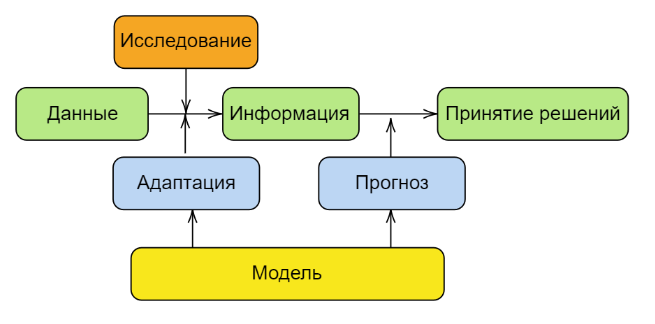
\includegraphics[width=6.25in,height=\textheight,keepaspectratio]{images/image.png}

}

\caption{Связь исследований и моделирования через процесс принятия
решений}

\end{figure}%

\begin{enumerate}
\def\labelenumi{\arabic{enumi}.}
\tightlist
\item
  Управление месторождениями строится на принятии решений. Принятие
  решений связано с необратимой тратой ресурсов с целью оптимизации
  некоторой целевой функции. Чаще всего целевая функция связана с
  экономикой проекта.
\item
  Исследования - инструмент для получения информации для принятия
  решений. Полезно разделить понятия данные и информация. Данные - то,
  что записано, информации - данные обработанные в контексте принятия
  решений.
\item
  Исследования основаны на моделях объекта управления. Модель -
  иструмент получения информации из данных. Также модель - инструмент
  принятия решений на основе информации. Модель - упрощенное
  представление реальности.
\item
  Модели используемые для принятия решений должны адекватно отражать
  реальность. Обеспечивается настройкой - адаптацией модели на известные
  данные и информацию. Такой процесс также можно считать исследованием.
  Почему?
\item
  Принятие решений на основе информации часто осуществляется на основе
  прогнозов - альтернативных вариантах принятия решений. Модель -
  инструмент для построения прогнозов.
\item
  В узком смысле - исследование скважины, в частности гидродинамические
  исследования - соответствуют адаптации специализированной модели -
  решения уравнения фильтрации. Адаптация готовит модель для построения
  прогнозов и принятия решений.
\item
  Понимание всей цепочки создания ценности от данных до принятия решений
  оказывается полезным, например для обоснования необходимости
  проведения исследований и оценки ценности информации получаемой в ходе
  исследований
\item
  Кроме понимания всей цепочки важно развитие навыков проведения
  расчетов - адаптации различных моделей, построения прогнозов с
  использованием этих моделей. Этому будет посвящена значительная часть
  курса.
\end{enumerate}

\begin{figure}[H]

{\centering \pandocbounded{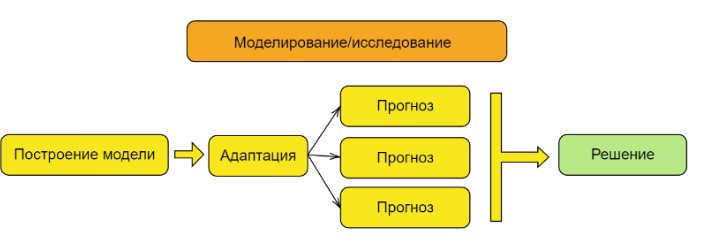
\includegraphics[keepaspectratio]{images/paste-1.png}}

}

\caption{Схема принятия решений с использованием моделей.}

\end{figure}%

\subsection{Инструменты для
моделирования}\label{ux438ux43dux441ux442ux440ux443ux43cux435ux43dux442ux44b-ux434ux43bux44f-ux43cux43eux434ux435ux43bux438ux440ux43eux432ux430ux43dux438ux44f}

Работа с моделями в ходе курса может проводиться с использованием
различного ПО

\begin{itemize}
\item
  python~для построения аналитических моделей

  Для работы можно использовать jupyter notebook или google colab или
  любой другой сервис для работы со скважинами. Потребуется освоить
  базовые библиотеки python - numpy, scipy, matplotlib, mpmath, pandas.
  Также будут использованы некоторые другие специализированные
  библиотеки.
\item
  Макросы MS Excel

  Часть расчетов можно выполнить с использованием макросов MS Excel,
  например Unifloc VBA (https://github.com/unifloc/unifloc\_vba)
\item
  Гидродинамический симулятор для построения численных моделей

  Базовый вариант - тНавигатор. Версия начиная от 19. Можно будет
  использовать другие симуляторы - РН-КИМ, Schlumberger eclipse, OPM и
  другие.
\item
  Специализированное ПО для анализа ГДИС

  Возможно, что то появится в ходе курса.
\end{itemize}

\section{Уравнение
фильтрации}\label{ux443ux440ux430ux432ux43dux435ux43dux438ux435-ux444ux438ux43bux44cux442ux440ux430ux446ux438ux438}

Уравнение фильтрации многофазного потока в пористой среде - основная
математическая модель пласта используемая в инженерных приложениях.
Используется не само уравнение, а разнообразные частные решения,
описывающие те или иные ситуации. Наиболее широко известным примером
решения уравнения фильтрации, возможно является, численное решение
которое строится трехмерными гидродинамическими симуляторами (eclipse,
tnavigator и так далее).

Как правило, при выводе уравнения фильтрации используются следующие
соотношения:

\begin{enumerate}
\def\labelenumi{\arabic{enumi}.}
\tightlist
\item
  закон Дарси - определяет линейную зависимость скорости фильтрации от
  давления
\end{enumerate}

\begin{equation}\phantomsection\label{eq-darcy_law_1}{ 
u_r=-\frac{k}{\mu}\frac{dp}{dr} 
}\end{equation}

\begin{enumerate}
\def\labelenumi{\arabic{enumi}.}
\setcounter{enumi}{1}
\item
  уравнение неразрывности - или закон сохранения массы, показывает что в
  потоке не могут образовываться разрывы сплошности:
  \begin{equation}\phantomsection\label{eq-mass_balance_1}{  
  \frac{1}{r}\frac{\partial\left(r\rho u_r\right)}{\partial r}=-\varphi\frac{\partial p}{\partial t} 
  }\end{equation}
\item
  уравнение состояния - задает зависимость плотности флюида от давления:
  \begin{equation}\phantomsection\label{eq-eos_1}{   
  c_0=\frac{1}{\rho}\frac{\partial\rho}{\partial p} 
  }\end{equation}
\end{enumerate}

Опираясь на эти соотношения уравнение фильтрации в радиальной форме
можно привести к виду для величин СИ.

\begin{equation}\phantomsection\label{eq-diff_eq_1}{ 
    \frac{\partial ^2 p }{\partial r^2} + \frac{1}{r} \frac{\partial p}{\partial r} = \frac{\varphi \mu c_t}{k} \frac{\partial p}{\partial t} 
}\end{equation}

Здесь используются следующие обозначения:

\begin{itemize}
\tightlist
\item
  \(u_r\) - скорость фильтрации в направлении \(r\), м/сек
\item
  \(k\) - проницаемость, м\(^2\)
\item
  \(\mu\) - вязкость флюида, Па с
\item
  \(p\) - давление, Па
\item
  \(r\) - расстояние, м
\item
  \(\rho\) - плотность флюида, кг/м\(^3\)
\item
  \(\varphi\) - пористость породы, доли единиц.
\item
  \(c_t\) - общая сжимаемость породы и флюида, 1/Па
\item
  \(t\) - время, сек
\end{itemize}

Иногда бывает удобно записать уравнение используя другие единицы
измерения, например практические метрические - уравнение примет вид:

\begin{tcolorbox}[enhanced jigsaw, opacityback=0, title=\textcolor{quarto-callout-tip-color}{\faLightbulb}\hspace{0.5em}{Уравнение фильтрации в практических метрических единицах измерений}, breakable, rightrule=.15mm, toptitle=1mm, left=2mm, bottomtitle=1mm, opacitybacktitle=0.6, colframe=quarto-callout-tip-color-frame, coltitle=black, titlerule=0mm, leftrule=.75mm, bottomrule=.15mm, arc=.35mm, colback=white, colbacktitle=quarto-callout-tip-color!10!white, toprule=.15mm]

\begin{equation}\phantomsection\label{eq-diff_eq_2}{ 
    \frac{\partial ^2 p }{\partial r^2} + \frac{1}{r} \frac{\partial p}{\partial r} = \frac{\varphi \mu c_t}{0.00036 k} \frac{\partial p}{\partial t} 
}\end{equation}

\begin{itemize}
\tightlist
\item
  \(k\) - проницаемость, мД
\item
  \(\mu\) - вязкость флюида, сП
\item
  \(p\) - давление, атм
\item
  \(r\) - расстояние, м
\item
  \(\rho\) - плотность флюида, кг/м\(^3\)
\item
  \(\varphi\) - пористость породы, доли единиц.
\item
  \(c_t\) - общая сжимаемость породы и флюида, 1/атм
\item
  \(t\) - время, час
\end{itemize}

\end{tcolorbox}

Вывод уравнения фильтрации основан на следующих предположениях:

\begin{itemize}
\tightlist
\item
  пласт однородный и изотропный - пористость и проницаемость одинаковы
  во всем пласте и во всех направлениях и не зависят от давления
\item
  добывающая скважина вскрывает весь продуктивный горизонт и
  обеспечивает радиальный приток к скважине
\item
  пласт насыщен одним флюидом на всем протяжении
\item
  температура не меняется в пласте, изотермичность
\end{itemize}

\subsection{Вывод уравнений
фильтрации}\label{ux432ux44bux432ux43eux434-ux443ux440ux430ux432ux43dux435ux43dux438ux439-ux444ux438ux43bux44cux442ux440ux430ux446ux438ux438}

\subsubsection{Вывод уравнения фильтрации для линейного
потока}\label{ux432ux44bux432ux43eux434-ux443ux440ux430ux432ux43dux435ux43dux438ux44f-ux444ux438ux43bux44cux442ux440ux430ux446ux438ux438-ux434ux43bux44f-ux43bux438ux43dux435ux439ux43dux43eux433ux43e-ux43fux43eux442ux43eux43aux430}

Уравнение фильтрации основано на трех основных уравнениях:

\begin{itemize}
\tightlist
\item
  законе сохранения массы
\item
  зависимости связывающей градиент давления с расходом, в простейшем
  виде это закон Дарси
\item
  уравнении состояния - зависимости связывающей сжимаемость флюида (и
  отчасти среды) и давлением
\end{itemize}

Выпишем эти уравнения, чтобы разобраться. В уравнениях будем
придерживаться обозначений принятых в международной литературе, в
частности в публикациях общества инженеров нефтяников SPE. Описание
обозначений, а также единиц измерения можно найти в Эрлагер
(2006)\marginpar{\begin{footnotesize}
\begin{CSLReferences}{2}{0}
\bibitem[\citeproctext]{ref-erlagerGidrodinamicheskieMetodyIssledovaniya2006}
Эрлагер, Роберт. 2006. \emph{Гидродинамические методы исследования
скважин}. М.--Ижевск: Институт компьютерных исследований.
\end{CSLReferences}
\vspace{2mm}\par\end{footnotesize}}.
Особое внимание на данном этапе стоит обратить на размерные коэффициенты
в уравнениях. С одной стороны записывая уравнения в СИ их можно
упростить и избежать части сложностей с переводными коэффициентами. С
другой стороны во многих источниках переводные коэффициенты интесивно
используются и это оказывается удобно при программной реализации
алгоритмов. В данном описании приведем перевод коэффициентов в
практические метрические единицы.

\paragraph{Закон сохранения
массы}\label{ux437ux430ux43aux43eux43d-ux441ux43eux445ux440ux430ux43dux435ux43dux438ux44f-ux43cux430ux441ux441ux44b}

В дифференциальной форме, для потока в направлении \(x\)

\begin{equation}\phantomsection\label{eq-mass_conserv_1}{
-f \dfrac{\partial \rho q_x}{\partial x} = A \dfrac{\partial(\rho \phi)}{\partial t} 
}\end{equation}

где

\begin{itemize}
\tightlist
\item
  \(f\) - размерный коэффициент, для практических метрических единиц
  \(f= 0.04167\), для американских промысловых \(f = 0.23394\)
\item
  \(\rho\) - плотность флюида, кг/м\(^3\), lbm/ft\(^3\)
\item
  \(q_x\) - объемный расход в направлении \(x\), м\(^3\)/сут, bbl/day,
  учитываем для практических метрических единиц \(1\) м\(^3\)/сут
  \(= 0.04167\) м\(^3\)/час и для промысловых американских \(1\) bbl/day
  \(= 0.23394\) ft\(^3\)/hr\\
\item
  x - координата, м, ft
\item
  \(\phi\) - пористость, доли единиц
\item
  \(t\) - время, часы
\item
  \(A\) - площадь, м\(^2\), ft\(^2\)
\end{itemize}

В перечне указаны размерности для промысловых метрических и американских
промысловых единиц измерений, там где они отличаются.

Для практических метрических единиц (\ref{eq-mass_conserv_1}) можно
записать в виде
\begin{equation}\phantomsection\label{eq-mass_conserv_2}{
-0.04167 \dfrac{ \partial (\rho q_x) }{\partial x} = A \dfrac{\partial(\rho \phi)}{\partial t} 
}\end{equation}

\paragraph{Закон
Дарси}\label{ux437ux430ux43aux43eux43d-ux434ux430ux440ux441ux438}

Простейшим вариантом задания зависимости между измением давления и
потоком флюида является линейная зависимость - закон Дарси. При этом
линейный множитель в зависимости - функция как коллектора
(проницаемость), так и свойств флюида (вязкость).

Закон Дарси в направлении \(x\).
\begin{equation}\phantomsection\label{eq-darcy_law_2}{ 
q_x = -  \dfrac{k_x A}{f\mu} \dfrac{\partial p}{\partial x} 
}\end{equation}

где

\begin{itemize}
\tightlist
\item
  \(f\) - размерный коэффициент, для практических метрических единиц
  \(f= 115.74\), для американских промысловых \(f = 887.2\)
\item
  \(k_x\) - проницаемость в направлении движения потока, мД
\item
  \(A\) - площадь, м\(^2\), ft\(^2\)
\item
  \(\mu\) - динамическая вязкость, сП
\item
  \(p\) - давление, атм, psi
\item
  \(x\) - координата движения потока, м
\end{itemize}

В практических метрических единицах измерения (\ref{eq-darcy_law_2})
будет иметь вид \begin{equation}\phantomsection\label{eq-darcy_law_3}{ 
q_x = -  \dfrac{k_x A}{115.74\mu} \dfrac{\partial p}{\partial x} 
}\end{equation}

Пытаясь проверить корректность вывода переводных коэффициентов
необходимо учесть что для единиц измерение СИ получим \(f=1\), а
необходимые переводные коэффициенты можно записать как:

\begin{itemize}
\tightlist
\item
  \(q\): \(1\) {[}м\(^3\)/сек{]} = \(543439\) {[}bbl/day{]} = \(86400\)
  {[}м\(^3\)/сут{]}
\item
  \(k\): \(1\) {[}м\(^2\){]} = \(1.01325 \cdot 10^{15}\) {[}мД{]}
\item
  \(\mu\): \(1\) {[}Па\(\cdot\)с{]} = \(1000\) {[}сП{]}
\item
  \(p\): \(1\) {[}Па{]} = \(0.0001450\) {[}psi{]} = \(0.00000987\)
  {[}атм{]}
\item
  \(x\): \(1\) {[}м{]} = \(3.28\) {[}ft{]}
\item
  \(A\): \(1\) {[}м\(^2\){]} = \(10.76\) {[}ft\(^2\){]}
\end{itemize}

\paragraph{Уравнение
состояния}\label{ux443ux440ux430ux432ux43dux435ux43dux438ux435-ux441ux43eux441ux442ux43eux44fux43dux438ux44f}

В простейшем варианте, который мы будет изучать, предполагается, что
сжимаемость постоянна и мала

\begin{equation}\phantomsection\label{eq-eos_2}{
c_t = c_{formation} + c_{fluid} = const
}\end{equation}

\begin{itemize}
\tightlist
\item
  \(c_t\) - общая сжимаемость (total compressibility)
\item
  \(c_{formation}\) - сжимаемость породы (formation compressibility),
  \(c_{formation} = \dfrac{1}{\phi}\dfrac{\partial \phi}{\partial p}\)
\item
  \(c_{fluid}\) - сжимаемость флюида (fluid compressibility),
  \(c_{fluid} = \dfrac{1}{\rho}\dfrac{\partial \rho}{\partial p}\)
\end{itemize}

\paragraph{Уравнение
фильтрации}\label{ux443ux440ux430ux432ux43dux435ux43dux438ux435-ux444ux438ux43bux44cux442ux440ux430ux446ux438ux438-1}

Подставим выражение для закона Дарси (\ref{eq-darcy_law_3}) в уравнение
мат баланса (\ref{eq-mass_conserv_2})

\begin{equation}\phantomsection\label{eq-diff_eq_2_}{ 
0.04167 \dfrac{ \partial}{\partial x} { \left[ \rho   \dfrac{k_x A}{115.74\mu} \dfrac{\partial p}{\partial x} \right] } = A \dfrac{\partial(\rho \phi)}{\partial t}  
}\end{equation}

Упрощая (\ref{eq-diff_eq_2}) получим

\begin{equation}\phantomsection\label{eq-diff_eq_3}{ 
\frac{\partial (\rho \phi)}{\partial t} = 0.00036 k_x \dfrac{ \partial}{\partial x}\left[ \dfrac{\rho}{\mu}\dfrac{\partial p}{\partial x} \right] 
}\end{equation}

Уравнение (\ref{eq-diff_eq_3}) подходит для потока газа. Для жидкости,
предполагая малую сжимаемость флюида можно его упростить до вида

\begin{equation}\phantomsection\label{eq-diff_eq_4}{ 
\frac{\partial p}{\partial t} = 0.00036 \dfrac{k_x}{\phi \mu c_t} \dfrac{ \partial^2 p}{\partial x^2} 
}\end{equation}

Напомним, здесь

\begin{itemize}
\tightlist
\item
  \(p\) - давление, атм
\item
  \(t\) - время, час
\item
  \(k_x\) - проницаемость в направлении движения потока, мД
\item
  \(\mu\) - динамическая вязкость, сП
\item
  \(\phi\) - пористость, д.е.
\item
  \(c_t\) - сжимаемость, 1/атм
\item
  \(x\) - расстояние, м
\end{itemize}

Приведенное уравнение (\ref{eq-diff_eq_4}) соответствует линейному
потоку в пласте. Практический интерес представляет решение для
радиального потока

\subsubsection{Вывод уравнения фильтрации для радиального
потока}\label{ux432ux44bux432ux43eux434-ux443ux440ux430ux432ux43dux435ux43dux438ux44f-ux444ux438ux43bux44cux442ux440ux430ux446ux438ux438-ux434ux43bux44f-ux440ux430ux434ux438ux430ux43bux44cux43dux43eux433ux43e-ux43fux43eux442ux43eux43aux430}

\marginnote{\begin{footnotesize}

\begin{figure}[H]

{\centering \pandocbounded{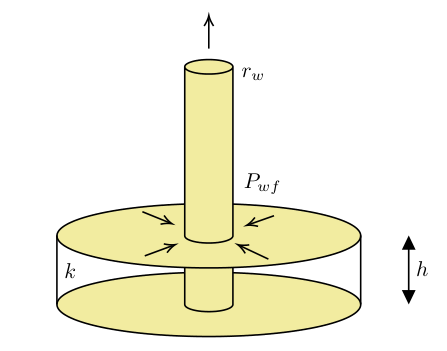
\includegraphics[keepaspectratio]{images/paste-2.png}}

}

\caption{Схема радиального притока к скважине}

\end{figure}%

\end{footnotesize}}

\paragraph{Закон сохранения
массы}\label{ux437ux430ux43aux43eux43d-ux441ux43eux445ux440ux430ux43dux435ux43dux438ux44f-ux43cux430ux441ux441ux44b-1}

Закон сохранения массы или принцип неразрывности можно выразить в
радиальной форме следующим соотношением

\begin{equation}\phantomsection\label{eq-mass_balance_2}{ 
\frac{1}{r}\frac{\partial\left(r\rho u_r\right)}{\partial r}=-\varphi\frac{\partial p}{\partial t}
}\end{equation}

Принцип неразрывности показывает, что для определенного объема пласта,
масса флюида которое втекла в контрольный объем пласта минус масса
которая вытекла равна массе которая накопилась в объеме.

Сохранение импульса или закон Дарси можно выразить соотношением

\begin{equation}\phantomsection\label{eq-darcy_law_4}{ 
 u_r=-\frac{k}{\mu}\frac{d^p}{dr}
}\end{equation}

Закон Дарси здесь используется как псевдоустановившаяся аппроксимация
обобщенного уравнения сохранения импульса (то есть слагаемым отвечающим
за накопление импульса пренебрегаем). Это предположение справедливо если
не учитывать возмущения давления в среде двигающиеся со скоростью звука.
Все изменения давления описываемые моделью связаны с локальными
изменениями градиента давления за счет ламинарного режима потока. Хотя
далее в модели будет учтена сжимаемость системы всеми ``звуковыми''
эффектами в системе мы пренебрегаем.

Поток предполагается горизонтальным, поэтому давление \(p\) может быть
использовано в качестве потенциала потока, гравитационными силами
пренебрегаем.

Комбинируя уравнения (\ref{eq-mass_balance_2}) , (\ref{eq-darcy_law_4})
получим:

\begin{equation}\phantomsection\label{eq-diff_eq_rad_1}{ 
\frac{1}{r}\frac{\partial\left( \dfrac{r\rho k}{\mu}\dfrac{\partial p}{dr}\right)}{\partial r}=\varphi\frac{\partial \rho}{\partial t}
}\end{equation}

Уравнение (\ref{eq-diff_eq_rad_1}) -- дифференциальное уравнение в
частных производных описывающее нестационарный поток однофазного флюида
в пористой среде при ламинарном потоке.

Вообще говоря приведенное уравнение является нелинейным, так как
плотность \(\rho = \rho(p)\) и вязкость \(\mu = \mu(p)\) являются
функциями давления. Уравнение содержит две зависимые переменные -
давление \(p\) и плотность \(\rho\). Поэтому для его решения необходимо
задать еще одно соотношение, каковым может быть уравнение состояния
флюида связывающее плотность флюида и давление \(\rho = \rho(p)\).

\paragraph{Флюид постоянной
сжимаемости}\label{ux444ux43bux44eux438ux434-ux43fux43eux441ux442ux43eux44fux43dux43dux43eux439-ux441ux436ux438ux43cux430ux435ux43cux43eux441ux442ux438}

Нестационарное поведение давления в пласте связано со сжимаемостью
системы. При изменении давления в какой то точке, часть флюида
сжимается, происходит накопление или отдача флюида, что вызывает
задержку в распространении изменения флюида. Несмотря на то, что
сжимаемость флюидов и породы малы и во многих случаях ими можно
пренебречь, это не верно для пластовых систем для добычи нефти. Большие
объемы пласта и флюидов и высокие давления компенсируют малость
сжимаемости и требуют ее учета.

Для однофазного флюида разумным является предположение постоянства
сжимаемости.

Сжимаемость можно определить как

\[
c=-\frac{1}{V} \left(  \frac{ \partial V}{ \partial p}  \right) 
\]

учтем, что

\[
 \rho = \frac{m}{V} 
\]

тогда получим

\[
c=\frac{1}{\rho} \left(  \frac{ \partial \rho}{ \partial p}  \right) 
\]

Для флюида с постоянной сжимаемостью, проинтегрировав приведенное
уравнение можно получить

\[
\rho = \rho_i e^{c(p-p_i)}
\]

где \(\rho_i\) плотность флюида при некотором заданном давлении \(p_i\)

Продифференцировав выражение для плотности по времени получим

\[
c \rho \frac{\partial p}{\partial t} = \frac{\partial \rho}{\partial t}
\]

Подставив это выражение в ранее полученное уравнение фильтрации
(\ref{eq-diff_eq_rad_1}) получим

\begin{equation}\phantomsection\label{eq-diff_eq_rad_2}{ 
\frac{1}{r}\frac{\partial\left( \dfrac{r\rho k}{\mu}\dfrac{\partial p}{dr}\right)}{\partial r}=\varphi c \rho \frac{\partial p}{\partial t}  
}\end{equation}

Приведенное дифференциальное уравнение в частных производных все еще
нелинейно, поскольку зависит от плотности \(\rho\)

\paragraph{Общая
сжимаемость}\label{ux43eux431ux449ux430ux44f-ux441ux436ux438ux43cux430ux435ux43cux43eux441ux442ux44c}

Если пористость не является постоянной величиной и меняется с давлением,
тогда слагаемое отвечающее за накопление флюида в пласте можно выразить
как

\[
\frac{\partial \varphi \rho}{\partial t} = \varphi \frac{\partial \rho}{\partial t}+ \rho \frac{\partial \varphi }{\partial t} = \varphi c_l \rho \frac{\partial p}{\partial t} + \rho \frac{\partial \varphi }{\partial t}  
\]

где \(c_l\) сжимаемость жидкости.

Определим сжимаемость породы как

\[
c_f = \frac{1}{\varphi} \frac{\partial \varphi}{\partial p}
\]

тогда

\[
\frac{\partial \varphi \rho}{\partial t}  = \varphi \rho (c_l + c_f) \frac{\partial p}{\partial t}   
\]

хотя пористость здесь является функцией давления - в первом приближении
мы можем считать ее константой равной пористости при некотором среднем
давлении в пласте. Это справедливо для маленькой сжимаемости породы, что
верно почти всегда.

Уравнение для сжимаемости можно еще уточнить, учтя что в пласте могут
находится различные флюиды - вода и нефть с насыщенностями \(s_w\) и
\(s_o\)

тогда

\[ 
c_l = s_o c_o + s_w c_w 
\]

тогда можно ввести общую сжимаемость системы

\[
 c_t = c_l + c_f = s_o c_o + s_w c_w  + c_f 
\]

Заметим, что проницаемость k в законе Дарси это не абсолютная
проницаемость, но относительная проницаемость по нефти при насыщенности
водой соответствующей связанной воде.

\[ 
k= k_o (s_{wc}) 
\]

\paragraph{Линеаризация уравнения
фильтрации}\label{ux43bux438ux43dux435ux430ux440ux438ux437ux430ux446ux438ux44f-ux443ux440ux430ux432ux43dux435ux43dux438ux44f-ux444ux438ux43bux44cux442ux440ux430ux446ux438ux438}

Раскрыв производную в левой части (\ref{eq-diff_eq_rad_2}) и
предположив, что \(\dfrac{\partial p}{\partial r}\) мало а следовательно
слагаемым \(r \rho c_t \left( \dfrac{\partial p}{\partial r} \right)^2\)
можно пренебречь, получим линеаризованное уравнения фильтрации

\begin{equation}\phantomsection\label{eq-diff_eq_lin}{
\frac{\partial^2 p}{\partial r^2} + \frac{1}{r} \frac{\partial p}{\partial r}= \frac{\varphi \mu c_t}{k} \frac{\partial p}{\partial t}
}\end{equation}

\subsection{Безразмерные
переменные}\label{ux431ux435ux437ux440ux430ux437ux43cux435ux440ux43dux44bux435-ux43fux435ux440ux435ux43cux435ux43dux43dux44bux435}

Часто для анализа уравнений неустановившейся фильтрации используются
безразмерные переменные. Мы будем использовать переменные в виде:

\[ 
r_D = \frac{r}{r_w} 
\]

\[ 
t_D = \frac{kt}{\varphi \mu c_t r_w^2}
\]

\[ 
p_D = \frac{2 \pi kh}{q_s B \mu} \left( p_i - p_{wf} \right) 
\]

\[ 
q_D = \frac{q}{q_{ref}} 
\]

Здесь использованы единицы измерения СИ.

\begin{itemize}
\tightlist
\item
  \(q_s\) - дебит скважины на поверхности, приведенный к нормальным
  условиям м3/с
\item
  \(\varphi\) - пористость, доли единиц
\item
  \(\mu\) - вязкость нефти в пласте, Па с
\item
  \(B\) - объемный коэффициент нефти, м3/м3
\item
  \(p_i\) - начальное давление в пласте, Па
\item
  \(p_{wf}\) - давление забойное, Па
\item
  \(c_t\) - общая сжимаемость системы в пласте, 1/Па
\end{itemize}

Использование безразмерных переменных позволяет упростить уравнение
фильтрации, которое примет вид

\[ 
\frac{\partial p_D}{ \partial t_D} = \frac{1}{r_D} \frac{ \partial{ \left( r_D \dfrac{\partial p_D}{ \partial r_D} \right) } }{ \partial{r_D} } 
\]

\[ 
\frac{\partial p_D}{ \partial t_D} = \dfrac{1}{r_D} \left[ \dfrac{\partial}{\partial r_D} \left( r_D \dfrac{ \partial p_D} {\partial r_D} \right) \right] 
\]

Решение этого уравнения - функция безразмерного давления от безразмерных
времени и расстояния \(p_D(r_D, t_D)\)

Для практических расчетов удобнее бывает использовать безразмерные
переменные полученные для практических метрических единиц измерения.

\begin{tcolorbox}[enhanced jigsaw, opacityback=0, title=\textcolor{quarto-callout-tip-color}{\faLightbulb}\hspace{0.5em}{Определение безразмерных переменных в практических метрических единицах}, breakable, rightrule=.15mm, toptitle=1mm, left=2mm, bottomtitle=1mm, opacitybacktitle=0.6, colframe=quarto-callout-tip-color-frame, coltitle=black, titlerule=0mm, leftrule=.75mm, bottomrule=.15mm, arc=.35mm, colback=white, colbacktitle=quarto-callout-tip-color!10!white, toprule=.15mm]

\[ 
r_D = \frac{r}{r_w} 
\]

\[ 
t_D = \frac{0.00036 kt}{\varphi \mu c_t r_w^2}
\]

\[ 
p_D = \frac{kh}{ 18.4 q_s B \mu} \left( p_i - p_{wf} \right) 
\]

\[ 
q_D = \frac{q}{q_{ref}} 
\]

Здесь использованы практические метрические единицы измерения.

\begin{itemize}
\tightlist
\item
  \(q_s\) - дебит скважины на поверхности, приведенный к нормальным
  условиям м3/сут
\item
  \(\varphi\) - пористость, доли единиц
\item
  \(\mu\) - вязкость нефти в пласте, сП
\item
  \(B\) - объемный коэффициент нефти, м3/м3
\item
  \(p_i\) - начальное давление в пласте, атм
\item
  \(p_{wf}\) - давление забойное, атм
\item
  \(c_t\) - общая сжимаемость системы в пласте, 1/атм
\end{itemize}

\end{tcolorbox}

Уравнение фильтрации для радиального потока в линеаризованном виде можно
записать в виде

\[ 
\frac{\partial p}{\partial t} = 0.00036 \dfrac{k}{\phi \mu c_t} \dfrac{1}{r} \left[ \dfrac{\partial}{\partial r} \left( r \dfrac{ \partial p} {\partial r} \right) \right]  
\]

Использование безразмерных переменных позволяет упростить уравнение
фильтрации, которое примет вид

\[ 
\frac{\partial p_D}{ \partial t_D} = \dfrac{1}{r_D} \left[ \dfrac{\partial}{\partial r_D} \left( r_D \dfrac{ \partial p_D} {\partial r_D} \right) \right] 
\]

Решение этого уравнения - функция безразмерного давления от безразмерных
времени и расстояния \(p_D(r_D, t_D)\)

\subsubsection{Расчет безразмерных переменных в Unifloc
VBA}\label{ux440ux430ux441ux447ux435ux442-ux431ux435ux437ux440ux430ux437ux43cux435ux440ux43dux44bux445-ux43fux435ux440ux435ux43cux435ux43dux43dux44bux445-ux432-unifloc-vba}

Несмотря на простоту определений безразмерных переменных их часто
приходится применять при проведении расчетов. Поэтому в надстройке
Unifloc VBA реализован набор функций расчета безразмерных переменных.

Эти функции начинаются с префикса transient\_def.

\begin{verbatim}
    transient_def_cd
    transient_def_cs_1atm
    transient_def_td
    transient_def_t_day
    transient_def_pd
    transient_def_pwf_atma
\end{verbatim}

Описания функций и из аргументов можно найти в руководстве пользователя
Unifloc VBA

\section{Стационарные решения уравнения
фильтрации}\label{ux441ux442ux430ux446ux438ux43eux43dux430ux440ux43dux44bux435-ux440ux435ux448ux435ux43dux438ux44f-ux443ux440ux430ux432ux43dux435ux43dux438ux44f-ux444ux438ux43bux44cux442ux440ux430ux446ux438ux438}

Широкое распространение на практике получили стационарные решения
уравнения фильтрации. Приведем некоторые из них.

\subsection{Решение для постоянного давления на круговой
границе}\label{ux440ux435ux448ux435ux43dux438ux435-ux434ux43bux44f-ux43fux43eux441ux442ux43eux44fux43dux43dux43eux433ux43e-ux434ux430ux432ux43bux435ux43dux438ux44f-ux43dux430-ux43aux440ux443ux433ux43eux432ux43eux439-ux433ux440ux430ux43dux438ux446ux435}

Рассматривается самая простая модель работы добывающей скважины -
радиальная стационарная фильтрация в однородном изотропном пласте
круговой формы. Скважина находится в центре пласта
(Рисунок~\ref{fig-radial_inflow_steady_state_1}). На границе пласта
поддерживается постоянное давление. Фактически это означает, что через
границу пласта идет поток жидкости, уравновешивающий дебит скважины.

Решение можно получить как решения уравнения фильтрации, учитывая
стационарность потока

\begin{equation}\phantomsection\label{eq-diff_eq_10}{  
    \frac{\partial ^2 p }{\partial r^2} + \frac{1}{r} \frac{\partial p}{\partial r} = 0
}\end{equation}

\begin{marginfigure}

\centering{

\pandocbounded{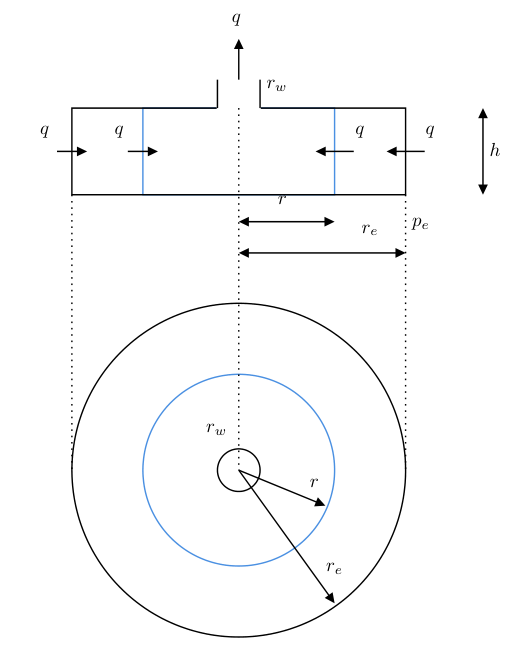
\includegraphics[keepaspectratio]{images/paste-3.png}}

}

\caption{\label{fig-radial_inflow_steady_state_1}Схема радиального
притока к скважине при наличии постоянного давления на границе}

\end{marginfigure}%

Или можно получить его непосредственно из закона Дарси, который должен
быть приведен к радиальной форме и в таком варианте известен как Формула
Дюпюи. Для приведенной конфигурации можно записать закон Дарси в форме.

\[
u_r=\frac{q}{2\pi rh}=\frac{k}{\mu}\frac{dP}{dr}
\]

Проинтегрировав выражение по замкнутому контуру радиуса \(r_e\) вокруг
скважины получим выражение известное как формула Дюпюи

\begin{equation}\phantomsection\label{eq-dupui_1}{ 
q=\frac{2\pi kh\left(P_e-P_w\right)}{\mu\left(\ln{\dfrac{r_e}{r_w}}\right)}
}\end{equation}

В приведенном выражения использованы единицы СИ.

Здесь

\begin{itemize}
\tightlist
\item
  \(u_r\) - приведенная скорость фильтрации на расстоянии \(r\) от
  скважины, м/с
\item
  \(q\) - объемные дебит скважины в рабочих условиях, м\(^3\)/с
\item
  \(r\) - радиус - расстояние от центра скважины, м
\item
  \(r_e\) - радиус зоны дренирования, на котором поддерживается
  постоянное давление, м
\item
  \(r_w\) - радиус скважины, на котором замеряется забойное давление, м
\item
  \(P\) - давление, Па
\item
  \(P_e\) - давление на внешнем контуре дренирования, Па
\item
  \(P_w\) - давление на забое скважины, Па
\item
  \(k\) - проницаемость, м\(^2\)
\item
  \(\mu\) - вязкость нефти в зоне дренирования, Па с
\end{itemize}

На практике часто бывает удобнее пользоваться значениями в практических
метрических единицах измерения.

\begin{equation}\phantomsection\label{eq-dupui_2}{
q=\frac{kh\left(P_e-P_w\right)}{ 18.4 \mu\left(\ln{\dfrac{r_e}{r_w}}\right)}
}\end{equation}

где

\begin{itemize}
\tightlist
\item
  \(q\) - объемные дебит скважины в рабочих условиях, м\(^3\)/сут
\item
  \(r\) - радиус - расстояние от центра скважины, м
\item
  \(r_e\) - радиус зоны дренирования, на котором поддерживается
  постоянное давление, м
\item
  \(r_w\) - радиус скважины, на котором замеряется забойное давление, м
\item
  \(P\) - давление, атм
\item
  \(P_e\) - давление на внешнем контуре дренирования, атм
\item
  \(P_w\) - давление на забое скважины, атм
\item
  \(k\) - проницаемость, мД
\item
  \(\mu\) - вязкость нефти в зоне дренирования, сП
\end{itemize}

Далее если не указано особо будем использовать практические метрические
единицы.

\subsection{Расчет решения с использованием
python}\label{ux440ux430ux441ux447ux435ux442-ux440ux435ux448ux435ux43dux438ux44f-ux441-ux438ux441ux43fux43eux43bux44cux437ux43eux432ux430ux43dux438ux435ux43c-python}

Для работы с решениями уравнения фильтрации удобно использовать язык
программирования python. Расчет на python может быть реализован на
основе библиотек numpy scipy.

\begin{Shaded}
\begin{Highlighting}[]
\CommentTok{"""}
\CommentTok{Импортируем библиотеки для расчетов. }
\CommentTok{numpy {-} для работы с массивами и подготовки данных }
\CommentTok{matplotlib {-} для построения графиков}
\CommentTok{scipy {-} для решения линейных уравнений}
\CommentTok{"""}
\ImportTok{import}\NormalTok{ numpy }\ImportTok{as}\NormalTok{ np}
\ImportTok{import}\NormalTok{ matplotlib.pyplot }\ImportTok{as}\NormalTok{ plt}
\ImportTok{import}\NormalTok{ scipy}
\end{Highlighting}
\end{Shaded}

Для удобства дальнейшего изложения и использования расчетных функций при
создании функций и переменных на языке python названия формируются по
следующим принципам:

\begin{itemize}
\tightlist
\item
  сначала указывается, что расчитывается в функции, в данном случае -
  давление \texttt{p} или \texttt{dp}
\item
  потом указываются пояснения - в данном случае \texttt{dp\_ss} - steady
  state pressure
\item
  в конце указывается размерность в которой ожидается получаение ответа
  - в данном случае \texttt{atma} - абсолютные атмосферы.
\end{itemize}

\begin{Shaded}
\begin{Highlighting}[]
\CommentTok{"""}
\CommentTok{Определим функции для расчета стационарного решения}
\CommentTok{"""}
\KeywordTok{def}\NormalTok{ dp\_ss\_atm(q\_liq\_sm3day }\OperatorTok{=} \DecValTok{50}\NormalTok{,}
\NormalTok{               mu\_cP }\OperatorTok{=} \DecValTok{1}\NormalTok{,}
\NormalTok{               b\_m3m3 }\OperatorTok{=} \FloatTok{1.2}\NormalTok{,}
\NormalTok{               kh\_mDm }\OperatorTok{=} \DecValTok{40}\NormalTok{,}
\NormalTok{               r\_e\_m }\OperatorTok{=} \DecValTok{240}\NormalTok{,}
\NormalTok{               r\_m }\OperatorTok{=} \FloatTok{0.1}\NormalTok{):}
  \CommentTok{"""}
\CommentTok{  функция расчета перепада давления в произвольной точке пласта }
\CommentTok{  на расстоянии r\_m от центра скважины для стационарного решения}
\CommentTok{  {-} q\_liq\_sm3day {-} дебит жидкости на поверхности в стандартных условиях}
\CommentTok{  {-} mu\_cP {-} вязкость нефти (в пластовых условиях)}
\CommentTok{  {-} B\_m3m3 {-} объемный коэффициент нефти }
\CommentTok{  {-} kh\_mDm {-} kh пласта}
\CommentTok{  {-} r\_e\_m {-} радиус контрура питания, м  }
\CommentTok{  {-} r\_m {-} расстояние на котором проводится расчет, м}
\CommentTok{  """}
  \ControlFlowTok{return} \FloatTok{18.42} \OperatorTok{*}\NormalTok{ q\_liq\_sm3day }\OperatorTok{*}\NormalTok{ mu\_cP }\OperatorTok{*}\NormalTok{ b\_m3m3}\OperatorTok{/}\NormalTok{ kh\_mDm }\OperatorTok{*}\NormalTok{ np.log(r\_e\_m}\OperatorTok{/}\NormalTok{r\_m)}

\KeywordTok{def}\NormalTok{ p\_ss\_atma(p\_res\_atma }\OperatorTok{=} \DecValTok{250}\NormalTok{,}
\NormalTok{              q\_liq\_sm3day }\OperatorTok{=} \DecValTok{50}\NormalTok{,}
\NormalTok{              mu\_cP }\OperatorTok{=} \DecValTok{1}\NormalTok{,}
\NormalTok{              b\_m3m3 }\OperatorTok{=} \FloatTok{1.2}\NormalTok{,}
\NormalTok{              k\_mD }\OperatorTok{=} \DecValTok{40}\NormalTok{,}
\NormalTok{              h\_m }\OperatorTok{=} \DecValTok{10}\NormalTok{,}
\NormalTok{              r\_e\_m }\OperatorTok{=} \DecValTok{240}\NormalTok{,}
\NormalTok{              r\_m }\OperatorTok{=} \FloatTok{0.1}\NormalTok{):}
  \CommentTok{"""}
\CommentTok{  функция расчета давления в произвольной точке пласта }
\CommentTok{  на расстоянии r\_m от центра скважины для стационарного решения }
\CommentTok{  {-} p\_res\_atma {-} пластовое давление, давление на контуре питания}
\CommentTok{  {-} q\_liq\_sm3day {-} дебит жидкости на поверхности в стандартных условиях}
\CommentTok{  {-} mu\_cP {-} вязкость нефти (в пластовых условиях)}
\CommentTok{  {-} B\_m3m3 {-} объемный коэффициент нефти }
\CommentTok{  {-} k\_mD {-} проницаемость пласта}
\CommentTok{  {-} h\_m {-} мощность пласта, м}
\CommentTok{  {-} r\_e\_m {-} радиус контрура питания, м  }
\CommentTok{  {-} r\_m {-} расстояние на котором проводится расчет, м}
\CommentTok{  """}
  \ControlFlowTok{return}\NormalTok{ p\_res\_atma }\OperatorTok{{-}}\NormalTok{ dp\_ss\_atm(q\_liq\_sm3day }\OperatorTok{=}\NormalTok{ q\_liq\_sm3day,}
\NormalTok{                                mu\_cP }\OperatorTok{=}\NormalTok{ mu\_cP,}
\NormalTok{                                b\_m3m3 }\OperatorTok{=}\NormalTok{ b\_m3m3,}
\NormalTok{                                kh\_mDm }\OperatorTok{=}\NormalTok{ k\_mD }\OperatorTok{*}\NormalTok{ h\_m,}
\NormalTok{                                r\_e\_m }\OperatorTok{=}\NormalTok{ r\_e\_m,}
\NormalTok{                                r\_m }\OperatorTok{=}\NormalTok{ r\_m)}
\end{Highlighting}
\end{Shaded}

Функции расчетов могут быть использованы для построения графиков,
например с использованием matplotlib

\marginnote{\begin{footnotesize}

\begin{Shaded}
\begin{Highlighting}[]
\CommentTok{"""}
\CommentTok{Построим график распределения давления в пласте}
\CommentTok{"""}
\CommentTok{\# формируем массив расстояний для которых будем проводить расчет}
\NormalTok{r\_arr }\OperatorTok{=}\NormalTok{ np.linspace(}\FloatTok{0.1}\NormalTok{, }\DecValTok{100}\NormalTok{, }\DecValTok{500}\NormalTok{) }

\CommentTok{\# рассчитываем массив давлений на соответствующих расстояниях}
\CommentTok{\# для расчета используется векторный расчет numpy {-} нет необходимости делать цикл в явном виде}
\CommentTok{\# для примера показана передача всех аргументов созданной функции}
\NormalTok{p\_arr }\OperatorTok{=}\NormalTok{ p\_ss\_atma(p\_res\_atma }\OperatorTok{=} \DecValTok{250}\NormalTok{,}
\NormalTok{                  q\_liq\_sm3day }\OperatorTok{=} \DecValTok{50}\NormalTok{,}
\NormalTok{                  mu\_cP }\OperatorTok{=} \DecValTok{1}\NormalTok{,}
\NormalTok{                  b\_m3m3 }\OperatorTok{=} \FloatTok{1.2}\NormalTok{,}
\NormalTok{                  k\_mD }\OperatorTok{=} \DecValTok{40}\NormalTok{,}
\NormalTok{                  h\_m }\OperatorTok{=} \DecValTok{10}\NormalTok{,}
\NormalTok{                  r\_e\_m }\OperatorTok{=} \DecValTok{240}\NormalTok{,}
\NormalTok{                  r\_m }\OperatorTok{=}\NormalTok{ r\_arr)}

\NormalTok{fig, (ax1, ax2) }\OperatorTok{=}\NormalTok{ plt.subplots(}\DecValTok{2}\NormalTok{, }\DecValTok{1}\NormalTok{, figsize}\OperatorTok{=}\NormalTok{(}\DecValTok{5}\NormalTok{,}\DecValTok{8}\NormalTok{))}

\CommentTok{\# рисуем график в обычных координатах}
\NormalTok{ax1.plot(r\_arr, p\_arr)   }\CommentTok{\# команда отрисовки графика по заданным массивам}
\NormalTok{ax1.plot(}\OperatorTok{{-}}\NormalTok{r\_arr, p\_arr)   }\CommentTok{\# отрицательная ветка}
\CommentTok{\# настраиваем график}

\NormalTok{ax1.set\_xlabel(}\StringTok{\textquotesingle{}r, m\textquotesingle{}}\NormalTok{)}
\NormalTok{ax1.set\_ylabel(}\StringTok{\textquotesingle{}p, atma\textquotesingle{}}\NormalTok{)}

\CommentTok{\# рисуем график в логарифмических координатах}
\NormalTok{ax2.plot(r\_arr, p\_arr)   }\CommentTok{\# команда отрисовки графика по заданным массивам}
\NormalTok{ax2.plot(}\OperatorTok{{-}}\NormalTok{r\_arr, p\_arr)   }\CommentTok{\# отрицательная ветка}
\CommentTok{\# настраиваем график}
\NormalTok{ax2.set\_xlabel(}\StringTok{\textquotesingle{}r, m\textquotesingle{}}\NormalTok{)}
\NormalTok{ax2.set\_xscale(}\StringTok{\textquotesingle{}symlog\textquotesingle{}}\NormalTok{, linthresh}\OperatorTok{=}\FloatTok{0.1}\NormalTok{, linscale}\OperatorTok{=}\FloatTok{0.6}\NormalTok{)}
\NormalTok{plt.show()}
\end{Highlighting}
\end{Shaded}

\begin{figure}[H]

\centering{

\pandocbounded{\includegraphics[keepaspectratio]{lecture_1_files/figure-pdf/fig-stac_pressure_dist_1-output-1.pdf}}

}

\caption{\label{fig-stac_pressure_dist_1}Распределение давления в
круговом пласте}

\end{figure}%

\end{footnotesize}}

\subsection{Учет скин-фактора для стационарного
решения}\label{ux443ux447ux435ux442-ux441ux43aux438ux43d-ux444ux430ux43aux442ux43eux440ux430-ux434ux43bux44f-ux441ux442ux430ux446ux438ux43eux43dux430ux440ux43dux43eux433ux43e-ux440ux435ux448ux435ux43dux438ux44f}

Скин-фактор --- гидродинамический параметр, характеризующий
дополнительное фильтрационное сопротивление течению флюидов в
околоскважинной зоне пласта, приводящее к изменению добычи (дебита) по
сравнению с совершенной (идеальной) скважиной. Скин-фактор может
приводить как к снижению дебита (например при загрязнении ПЗС), так и
увеличению (образование высокопроводящих каналов в ПЗС).

Концепция скин-фактора получила широкое распространение на практике. Все
инженеры-нефтяники знают этот параметр и оперируют им на практике.

Изначально скин-фактор был введен как параметр учитывающий изменение
проницаемости (загрязнение) призабойной зоны при расчете
производительности скважины. Такое загрязнение может быть вызвано
различными причинами:

\begin{itemize}
\tightlist
\item
  проникновением бурового раствора в пласт и блокировкой поровых
  каналов;
\item
  набуханием глин при контакте с фильтратом бурового раствора;
\item
  химическим осаждением элементов бурового раствора, жидкости глушения
  или пластовых флюидов в призабойной зоне скважины, например осаждением
  солей или асфальтенов;
\item
  продвижением песчаных частиц к стволу скважины;
\item
  повреждением породы при перфорации;
\item
  другими причинами.
\end{itemize}

Для модели загрязненной призабойной зоны величину скин-фактора можно
выразить формулой Хокинса (Hawkins
1956)\marginpar{\begin{footnotesize}
\begin{CSLReferences}{2}{0}
\bibitem[\citeproctext]{ref-hawkinsNoteSkinEffect1956}
Hawkins, Murray F. 1956. {«A {Note} on the {Skin Effect}»}.
\emph{Journal of Petroleum Technology} 8 (12): 65--66.
\url{https://doi.org/10.2118/732-G}.
\end{CSLReferences}
\vspace{2mm}\par\end{footnotesize}}.
Скин-фактор для плоскорадиального установившегося потока несжимаемой
жидкости:

\begin{equation}\phantomsection\label{eq-skin_hokins}{ 
S =\left( \frac{k}{k_s} -1\right)\ ln\frac{r_s}{r_w}
}\end{equation}

здесь:

\begin{itemize}
\tightlist
\item
  \(k_s\) - проницаемость в загрязненной ПЗП;
\item
  \(k\) - однородная проницаемость по всему пласту;
\item
  \(r_s\) - радиус загрязненной зоны;
\item
  \(r_w\) - радиус скважины.
\end{itemize}

Концепция скин-фактора оказалась удобной для описания характеристики
соединения скважины и пласта и была распространена на другие случаи,
когда производительность скважины могла отличаться от производительности
идеальной скважины:

\begin{itemize}
\tightlist
\item
  для горизонтальных скважин;
\item
  для скважин вскрывающих пласт под углом;
\item
  для скважин пересеченных трещиной ГРП;
\item
  для скважин вскрытых перфорацией и учета гидравлического сопротивления
  потока на перфорационных отверстиях;
\item
  другими причинами.
\end{itemize}

Для многих подобных случаев предположение о радиальном притоке к
скважине не верно, но величину скин-фактора используют, так как она
позволяет сравнить производительность скважины со сложным заканчиванием
с простой вертикальной скважиной. В таких случая говорят о
псевдорадиальном скин-факторе - такой величине скин-фактора \(S\),
которая обеспечила бы такую же производительность для вертикальной
скважины полностью вскрывающей пласт.

Для стационарной радиальной модели притока учет скин-фактора приведен к
следующим соотношениям:

\begin{equation}\phantomsection\label{eq-dupui_skin_1}{ 
(P_e - P_{wf}) = \frac{18.42\mu q }{\ k h}(\ln\frac{r_e}{r_w}+S) 
}\end{equation}

\begin{equation}\phantomsection\label{eq-dupui_skin_2}{ 
q=\frac{kh\left(P_e-P_w\right)}{ 18.42 \mu\left(\ln{\dfrac{r_e}{r_w}} + S\right)}
}\end{equation}

\subsection{Решение для постоянного давления на круговой границе с
учетом среднего давления в области
дренирования}\label{ux440ux435ux448ux435ux43dux438ux435-ux434ux43bux44f-ux43fux43eux441ux442ux43eux44fux43dux43dux43eux433ux43e-ux434ux430ux432ux43bux435ux43dux438ux44f-ux43dux430-ux43aux440ux443ux433ux43eux432ux43eux439-ux433ux440ux430ux43dux438ux446ux435-ux441-ux443ux447ux435ux442ux43eux43c-ux441ux440ux435ux434ux43dux435ux433ux43e-ux434ux430ux432ux43bux435ux43dux438ux44f-ux432-ux43eux431ux43bux430ux441ux442ux438-ux434ux440ux435ux43dux438ux440ux43eux432ux430ux43dux438ux44f}

\marginnote{\begin{footnotesize}

\begin{Shaded}
\begin{Highlighting}[]
\CommentTok{\# оценим среднее давление в области дренирования}
\NormalTok{r\_external\_m }\OperatorTok{=} \DecValTok{240}
\NormalTok{r\_well\_m }\OperatorTok{=} \FloatTok{0.1}
\NormalTok{p\_average\_atma }\OperatorTok{=}\NormalTok{ scipy.integrate.quad(}\KeywordTok{lambda}\NormalTok{ r:p\_ss\_atma(p\_res\_atma}\OperatorTok{=}\DecValTok{250}\NormalTok{,}
\NormalTok{                                                         q\_liq\_sm3day}\OperatorTok{=}\DecValTok{50}\NormalTok{,}
\NormalTok{                                                         mu\_cP}\OperatorTok{=}\DecValTok{1}\NormalTok{,}
\NormalTok{                                                         b\_m3m3}\OperatorTok{=}\FloatTok{1.2}\NormalTok{,}
\NormalTok{                                                         k\_mD}\OperatorTok{=}\DecValTok{40}\NormalTok{,}
\NormalTok{                                                         h\_m}\OperatorTok{=}\DecValTok{10}\NormalTok{,}
\NormalTok{                                                         r\_e\_m}\OperatorTok{=}\NormalTok{r\_external\_m,}
\NormalTok{                                                         r\_m}\OperatorTok{=}\NormalTok{r) }\OperatorTok{*} \DecValTok{2}  \OperatorTok{*}\NormalTok{ r, }
\NormalTok{                                      r\_well\_m, }
\NormalTok{                                      r\_external\_m)[}\DecValTok{0}\NormalTok{]   }\OperatorTok{/}\NormalTok{ r\_external\_m}\OperatorTok{**}\DecValTok{2} 
\BuiltInTok{print}\NormalTok{(}\SpecialStringTok{f"p\_average\_atma = }\SpecialCharTok{\{}\NormalTok{p\_average\_atma}\SpecialCharTok{\}}\SpecialStringTok{"}\NormalTok{)}

\NormalTok{r\_arr }\OperatorTok{=}\NormalTok{ np.linspace(r\_well\_m, r\_external\_m, }\DecValTok{500}\NormalTok{)}
\NormalTok{r\_full }\OperatorTok{=}\NormalTok{ np.linspace(}\OperatorTok{{-}}\NormalTok{r\_external\_m, r\_external\_m, }\DecValTok{10}\NormalTok{) }

\CommentTok{\# рассчитываем массив давлений на соответствующих расстояниях}
\CommentTok{\# для расчета используется векторный расчет numpy {-} нет необходимости делать цикл в явном виде}
\CommentTok{\# для примера показана передача всех аргументов созданной функции}
\NormalTok{p\_arr }\OperatorTok{=}\NormalTok{ p\_ss\_atma(p\_res\_atma}\OperatorTok{=}\DecValTok{250}\NormalTok{,}
\NormalTok{                  q\_liq\_sm3day}\OperatorTok{=}\DecValTok{50}\NormalTok{,}
\NormalTok{                  mu\_cP}\OperatorTok{=}\DecValTok{1}\NormalTok{,}
\NormalTok{                  b\_m3m3}\OperatorTok{=}\FloatTok{1.2}\NormalTok{,}
\NormalTok{                  k\_mD}\OperatorTok{=}\DecValTok{40}\NormalTok{,}
\NormalTok{                  h\_m}\OperatorTok{=}\DecValTok{10}\NormalTok{,}
\NormalTok{                  r\_e\_m}\OperatorTok{=}\NormalTok{r\_external\_m,}
\NormalTok{                  r\_m}\OperatorTok{=}\NormalTok{r\_arr)}

\NormalTok{fig, (ax1, ax2) }\OperatorTok{=}\NormalTok{ plt.subplots(}\DecValTok{2}\NormalTok{, }\DecValTok{1}\NormalTok{, figsize}\OperatorTok{=}\NormalTok{(}\DecValTok{8}\NormalTok{,}\DecValTok{8}\NormalTok{))}

\CommentTok{\# рисуем график в обычных координатах}
\NormalTok{ax1.plot(r\_arr, p\_arr)   }\CommentTok{\# команда отрисовки графика по заданным массивам}
\NormalTok{ax1.plot(}\OperatorTok{{-}}\NormalTok{r\_arr, p\_arr)}
\NormalTok{ax1.plot(r\_full, np.full\_like(r\_full, p\_average\_atma), linestyle}\OperatorTok{=}\StringTok{\textquotesingle{}dashed\textquotesingle{}}\NormalTok{)}
\CommentTok{\# настраиваем график}
\CommentTok{\#ax1.set\_title(\textquotesingle{}Воронка депрессии {-} распределение давления в пласте\textquotesingle{})}
\CommentTok{\#ax1.set\_xlabel(\textquotesingle{}r, m\textquotesingle{})}
\NormalTok{ax1.set\_ylabel(}\StringTok{\textquotesingle{}p, atma\textquotesingle{}}\NormalTok{)}

\CommentTok{\# рисуем график в логарифмических координатах}
\NormalTok{ax2.plot(r\_arr, p\_arr)   }\CommentTok{\# команда отрисовки графика по заданным массивам}
\NormalTok{ax2.plot(}\OperatorTok{{-}}\NormalTok{r\_arr, p\_arr) }
\NormalTok{ax2.plot(r\_full, np.full\_like(r\_full, p\_average\_atma), linestyle}\OperatorTok{=}\StringTok{\textquotesingle{}dashed\textquotesingle{}}\NormalTok{)}
\CommentTok{\# настраиваем график}
\CommentTok{\#ax2.set\_title(\textquotesingle{}Воронка депрессии {-} распределение давления в пласте\textquotesingle{})}
\NormalTok{ax2.set\_xlabel(}\StringTok{\textquotesingle{}r, m\textquotesingle{}}\NormalTok{)}
\NormalTok{ax2.set\_ylabel(}\StringTok{\textquotesingle{}p, atma\textquotesingle{}}\NormalTok{)}
\NormalTok{ax2.set\_xscale(}\StringTok{\textquotesingle{}symlog\textquotesingle{}}\NormalTok{, linthresh}\OperatorTok{=}\FloatTok{0.1}\NormalTok{, linscale}\OperatorTok{=}\FloatTok{0.6}\NormalTok{)}
\NormalTok{plt.show()}
\end{Highlighting}
\end{Shaded}

\begin{verbatim}
p_average_atma = 248.6184605726843
\end{verbatim}

\begin{figure}[H]

\centering{

\pandocbounded{\includegraphics[keepaspectratio]{lecture_1_files/figure-pdf/fig-radial_inflow_steady_state_2-output-2.pdf}}

}

\caption{\label{fig-radial_inflow_steady_state_2}Распределение давления
в круговом пласте и среднее давление}

\end{figure}%

\end{footnotesize}}

В приведенное выражение входит значение давления на контуре, которым не
всегда бывает удобно пользоваться. В практических случаях значение на
контуре трудно оценить, контур зоны дренирования может значительно
отличаться от кругового, да и радиус оценить может быть сложно. Удобнее
пользоваться средним давлением в зоне дренирования \(\bar{P}\), которое
может быть оценено по материальному балансу (смотри рисунок
\ref{fig-radial_inflow_steady_state_2}).

Вывод уравнения фильтрации для постоянного давления на границе с
использованием среднего давления

В этом случае выражение для дебита примет вид
\begin{equation}\phantomsection\label{eq-dupui_skin_aver_press}{
q=\frac{kh\left( \bar{P}-P_w\right)}{ 18.42 \mu\left(\ln{\dfrac{r_e}{r_w}}  - \dfrac{1}{2}+ S \right)}
}\end{equation}

\subsection{Решение для круговой непроницаемой
границы}\label{ux440ux435ux448ux435ux43dux438ux435-ux434ux43bux44f-ux43aux440ux443ux433ux43eux432ux43eux439-ux43dux435ux43fux440ux43eux43dux438ux446ux430ux435ux43cux43eux439-ux433ux440ux430ux43dux438ux446ux44b}

Схема модели радиального притока для условия непротекания на круговой
границе приведена на рисунке \ref{fig-radial_inflow_steady_state_3}

\begin{marginfigure}

\centering{

\pandocbounded{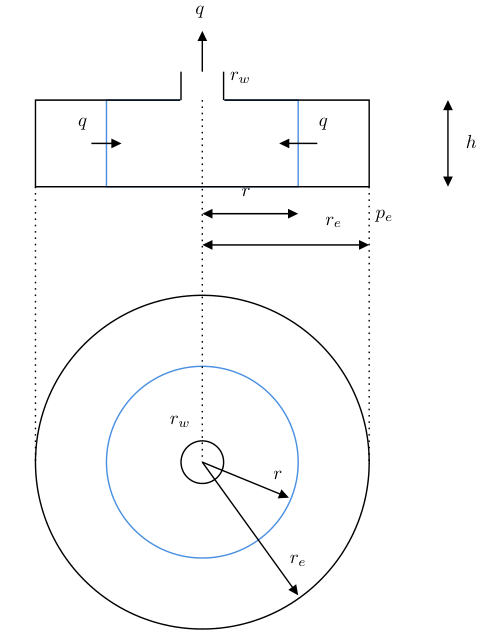
\includegraphics[keepaspectratio]{images/paste-5.png}}

}

\caption{\label{fig-radial_inflow_steady_state_3}Схема радиального
притока к скважине при наличии непроницаемой границы}

\end{marginfigure}%

При условии непротекания давления на границе условия стационарности
(неизменности давления) не достигаются. При работе скважины с постоянным
дебитом забойное давление будет постоянно снижаться. Однако начиная с
некоторого момента, когда влияние скважины достигнет границ - давление в
всей области дренирования начнет снижаться равномерно (смотри
Рисунок~\ref{fig-radial_pss_dynamics}).

\begin{figure}

\centering{

\pandocbounded{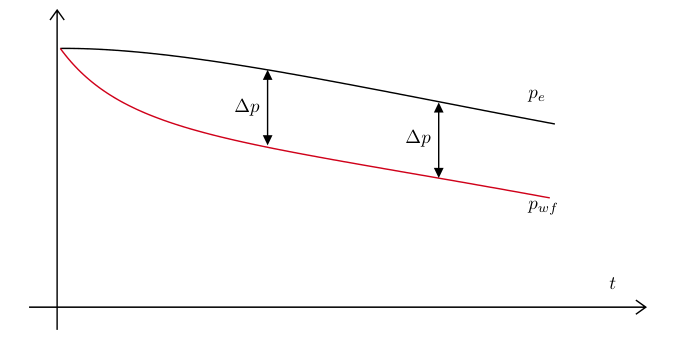
\includegraphics[keepaspectratio]{images/paste-6.png}}

}

\caption{\label{fig-radial_pss_dynamics}Изменение давления на границе и
на забое скважины во времени}

\end{figure}%

Такой режим, при котором забойное давление меняется, но перепад давления
\(P_e - P_w\) остается постоянным называют псевдо-установившимся режимом
работы (pss - pseudo steady state).

Для псевдо-установившегося режима можно записать выражение

\begin{equation}\phantomsection\label{eq-dupui_pss}{
q=\frac{kh\left(P_e-P_w\right)}{ 18.42 \mu\left(\ln{\dfrac{r_e}{r_w}} - \dfrac{1}{2} + S\right)}
}\end{equation} где

\begin{itemize}
\tightlist
\item
  \(q\) - объемные дебит скважины в рабочих условиях, м3/сут;
\item
  \(r\) - радиус - расстояние от центра скважины, м;
\item
  \(r_e\) - радиус зоны дренирования, на котором поддерживается
  постоянное давление, м;
\item
  \(r_w\) - радиус скважины, на котором замеряется забойное давление, м;
\item
  \(P\) - давление, атм;
\item
  \(P_e\) - давление на внешнем контуре дренирования, атм;
\item
  \(P_w\) - давление на забое скважины, атм;
\item
  \(k\) - проницаемость, мД;
\item
  \(\mu\) - вязкость нефти в зоне дренирования, сП.
\end{itemize}

\subsection{Решение для круговой непроницаемой границы с учетом среднего
давления в зоне
дренирования}\label{ux440ux435ux448ux435ux43dux438ux435-ux434ux43bux44f-ux43aux440ux443ux433ux43eux432ux43eux439-ux43dux435ux43fux440ux43eux43dux438ux446ux430ux435ux43cux43eux439-ux433ux440ux430ux43dux438ux446ux44b-ux441-ux443ux447ux435ux442ux43eux43c-ux441ux440ux435ux434ux43dux435ux433ux43e-ux434ux430ux432ux43bux435ux43dux438ux44f-ux432-ux437ux43eux43dux435-ux434ux440ux435ux43dux438ux440ux43eux432ux430ux43dux438ux44f}

Аналогично случаю для постоянного давления на границе можно переписать
выражение с использованием среднего давления в области дренирования.

\begin{equation}\phantomsection\label{eq-dupui_pss_aver_press}{
q=\frac{kh\left( \bar{P}-P_w\right)}{ 18.42 \mu\left(\ln{\dfrac{r_e}{r_w}} - \dfrac{3}{4}+ S \right)}
}\end{equation}

Вывод уравнений для псевдо-установившегося режима работы

\subsection{Стационарные решения для вертикальной скважины в резервуаре
произвольной
формы}\label{ux441ux442ux430ux446ux438ux43eux43dux430ux440ux43dux44bux435-ux440ux435ux448ux435ux43dux438ux44f-ux434ux43bux44f-ux432ux435ux440ux442ux438ux43aux430ux43bux44cux43dux43eux439-ux441ux43aux432ux430ux436ux438ux43dux44b-ux432-ux440ux435ux437ux435ux440ux432ux443ux430ux440ux435-ux43fux440ux43eux438ux437ux432ux43eux43bux44cux43dux43eux439-ux444ux43eux440ux43cux44b}

Здесь уравнения и методы расчета для горизонтальных, наклонно
направленных скважин, скважин с ГРП, горизонтальных скважин с МГРП.

\begin{equation}\phantomsection\label{eq-dupui_pss_form_factor}{
    q=\frac{kh\left( \bar{P}-P_w\right)}{ 18.42 \mu\left(\ln{\dfrac{2.2458 A}{C_A r_w^2}} + S \right)}
}\end{equation}

\begin{itemize}
\tightlist
\item
  \(q\) - объемные дебит скважины в рабочих условиях, м3/сут;
\item
  \(A\) - площадь области дренирования, м\(^2\);
\item
  \(C_A\) - фактор формы, зависит от формы резервуара и расположения
  скважины;
\item
  \(r_w\) - радиус скважины, на котором замеряется забойное давление, м;
\item
  \(\bar{P}\) - среднее давление в области дренирования, атм;
\item
  \(P_e\) - давление на внешнем контуре дренирования, атм;
\item
  \(P_w\) - давление на забое скважины, атм;
\item
  \(k\) - проницаемость, мД;
\item
  \(\mu\) - вязкость нефти в зоне дренирования, сП.
\end{itemize}

\begin{figure}

\centering{

\pandocbounded{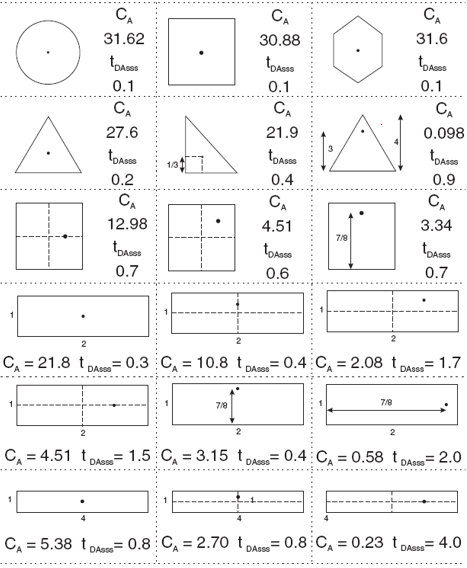
\includegraphics[keepaspectratio]{images/paste-7.png}}

}

\caption{\label{fig-shape_factors}Значения фактора формы}

\end{figure}%

\%todo -надо переделать рисунок и добавить ссылки на источники

Безразмерное время достижения псевдо-установившегося режима притока,
определяемое видом резервуара

\begin{equation}\phantomsection\label{eq-td_pss}{ 
t_{DApss} = \frac{kt_{pss}}{\varphi \mu c_t A} 
}\end{equation}

\subsection{Формула
Дюпюи}\label{ux444ux43eux440ux43cux443ux43bux430-ux434ux44eux43fux44eux438}

Простое решение для задачи стационарного притока к вертикальной скважине
в однородном изотропном пласте круговой формы с постоянным давлением на
границе имеет вид

\begin{equation}\phantomsection\label{eq-dupui_2}{
    Q=\dfrac{kh}{18.42\mu B} \dfrac{P_{res}-P_{wf}}{\ln \dfrac{r_e}{r_w} + S} 
}\end{equation}

где:

\begin{itemize}
\tightlist
\item
  \(Q\) - дебит скважины на поверхности, приведённый к нормальным
  условиям, ст. м\(^3\)/сут
\item
  \(\mu\) - вязкость нефти в пласте, сП
\item
  \(B\) - объёмный коэффициент нефти, м\(^3\)/м\(^3\)
\item
  \(P_{res}\) - пластовое давление или давление на контуре с радиусом
  \(r_e\), атма
\item
  \(P_{wf}\) - давление забойное, атма
\item
  \(k\) - проницаемость, мД
\item
  \(h\) - мощность пласта, м
\item
  \(r_e\) - внешний контур дренирования скважины, м
\item
  \(r_w\) - радиус скважины, м
\item
  \(S\) - скин-фактор скважины, безразм.
\end{itemize}

Это решение известно как закон Дарси
\url{https://ru.wikipedia.org/wiki/Закон_Дарси} или формула Дюпюи.

Выражение можно переписать в виде

\begin{equation}\phantomsection\label{eq-dupui_3}{
    P_{r} = P_{res} - 18.42\dfrac{ Q\mu B }{kh} \left[ \ln\dfrac{r_e}{r} +S \right]
}\end{equation}

который удобен для расчёта распределения давления в пласте \(P_r\) на
произвольном расстоянии от скважины \(r\). В выражении (2) задано
граничное значение давления \(p_e\) на контуре \(r_e\). Расчёт позволит
найти любое значение внутри контура, в том числе и забойное давление
\(P_{wf}\) на \(r=r_w\)

Выражение можно переписать
\begin{equation}\phantomsection\label{eq-dupui_4}{
    P_{r} = P_{wf} + 18.42\dfrac{ Q\mu B }{kh} \left[ \ln\dfrac{r}{r_w} +S \right]
}\end{equation}

где по известному дебиту и забойному давлению можно найти давление в
пласте. При известном пластовом давлении можно оценить радиус контура на
котором оно достигается.

\subsubsection{Формула Дюпюи в декартовых
координатах}\label{ux444ux43eux440ux43cux443ux43bux430-ux434ux44eux43fux44eux438-ux432-ux434ux435ux43aux430ux440ux442ux43eux432ux44bux445-ux43aux43eux43eux440ux434ux438ux43dux430ux442ux430ux445}

Для построения карты распределения давлений в пласте полезно вспомнить,
что расстояние от скважины с координатами \((x_{well}, y_{well})\) до
произвольной точки пласта с координатами \((x,y)\) можно найти по
формуле

\marginnote{\begin{footnotesize}

\begin{Shaded}
\begin{Highlighting}[]
\CommentTok{"""}
\CommentTok{Построим карту или сетку распределения давления в пласте}
\CommentTok{с использованием векторных функций numpy}
\CommentTok{"""}
\CommentTok{\# зададим параметры воронки депрессии}
\NormalTok{pres }\OperatorTok{=} \DecValTok{250} 
\NormalTok{r\_e }\OperatorTok{=} \DecValTok{300}

\CommentTok{\# зададим координатную сетку основываясь на параметрах}
\NormalTok{x }\OperatorTok{=}\NormalTok{ np.linspace(}\OperatorTok{{-}}\NormalTok{r\_e, r\_e, }\DecValTok{300}\NormalTok{)}
\NormalTok{y }\OperatorTok{=}\NormalTok{ np.linspace(}\OperatorTok{{-}}\NormalTok{r\_e, r\_e, }\DecValTok{300}\NormalTok{)}
\CommentTok{\# рассчитаем вспомогательные вектора для построения сетки}
\NormalTok{xv, yv }\OperatorTok{=}\NormalTok{ np.meshgrid(x, y)}
\CommentTok{\# зададим координаты скважины}
\NormalTok{xwell1 }\OperatorTok{=} \DecValTok{0}
\NormalTok{ywell1 }\OperatorTok{=} \DecValTok{0}
\CommentTok{\# рассчитаем значение давлений во всех точках сетки}
\CommentTok{\# расчет ведется для матрицы координата с использованием векторных возможностей numpy}
\NormalTok{p\_mesh }\OperatorTok{=}\NormalTok{ p\_ss\_atma(r\_m}\OperatorTok{=}\NormalTok{((xv}\OperatorTok{{-}}\NormalTok{xwell1)}\OperatorTok{**}\DecValTok{2} \OperatorTok{+}\NormalTok{ (yv}\OperatorTok{{-}}\NormalTok{ywell1)}\OperatorTok{**}\DecValTok{2}\NormalTok{)}\OperatorTok{**}\FloatTok{0.5}\NormalTok{, p\_res\_atma}\OperatorTok{=}\NormalTok{pres, r\_e\_m}\OperatorTok{=}\NormalTok{r\_e)}
\CommentTok{\# удалим значения за контуром, так как в данном случае они не имеют смысла}
\NormalTok{p\_mesh[np.where(p\_mesh }\OperatorTok{\textgreater{}}\NormalTok{ pres)] }\OperatorTok{=}\NormalTok{ pres}
\CommentTok{\# построим отображение в виде контурной карты}
\NormalTok{plt.rcParams[}\StringTok{"figure.figsize"}\NormalTok{] }\OperatorTok{=}\NormalTok{ (}\DecValTok{7}\NormalTok{,}\DecValTok{7}\NormalTok{)}
\NormalTok{plt.contour(x, y, p\_mesh, levels}\OperatorTok{=}\DecValTok{100}\NormalTok{)}
\NormalTok{plt.show()}
\end{Highlighting}
\end{Shaded}

\begin{figure}[H]

\centering{

\pandocbounded{\includegraphics[keepaspectratio]{lecture_1_files/figure-pdf/fig-stac_pressure_map_1-output-1.pdf}}

}

\caption{\label{fig-stac_pressure_map_1}Карта изолиний давления в
пласте}

\end{figure}%

\end{footnotesize}}

\begin{equation}\phantomsection\label{eq-r_from_x}{
r=\sqrt{ (x-x_{well})^2 + (y-y_{well})^2 }
}\end{equation}

Тогда выражение для расчета давления в любой точке пласта примет вид

\begin{equation}\phantomsection\label{eq-dupui__xy}{
    P_{r} = P_{res} - 18.42\dfrac{ Q\mu B }{kh} \left[ \ln\dfrac{r_e}{\sqrt{ (x-x_{well})^2 + (y-y_{well})^2 }} +S \right]
}\end{equation}

Простой вариант расчета - можно создать пустую матрицу со значениями
давления по сетке и перебирая все точки на сетке/матрице рассчитать
давления

\subsection{Суперпозиция для стационарного
решения}\label{ux441ux443ux43fux435ux440ux43fux43eux437ux438ux446ux438ux44f-ux434ux43bux44f-ux441ux442ux430ux446ux438ux43eux43dux430ux440ux43dux43eux433ux43e-ux440ux435ux448ux435ux43dux438ux44f}

\subsubsection{Суперпозиция для нескольких скважин с постоянным
дебитом}\label{ux441ux443ux43fux435ux440ux43fux43eux437ux438ux446ux438ux44f-ux434ux43bux44f-ux43dux435ux441ux43aux43eux43bux44cux43aux438ux445-ux441ux43aux432ux430ux436ux438ux43d-ux441-ux43fux43eux441ux442ux43eux44fux43dux43dux44bux43c-ux434ux435ux431ux438ux442ux43eux43c}

\marginnote{\begin{footnotesize}

\begin{Shaded}
\begin{Highlighting}[]
\CommentTok{"""}
\CommentTok{Построим карту или сетку распределения давления в пласте}
\CommentTok{для ряда/галереи скважин}
\CommentTok{"""}
\CommentTok{\# зададим параметры воронки депрессии}
\NormalTok{pres }\OperatorTok{=} \DecValTok{250} 
\NormalTok{r\_e }\OperatorTok{=} \DecValTok{300}

\CommentTok{\# зададим координаты скважины (всего будет 5 скважин у которых меняется только х координата)}
\NormalTok{xwell }\OperatorTok{=}\NormalTok{ [}\OperatorTok{{-}}\DecValTok{100}\NormalTok{, }\OperatorTok{{-}}\DecValTok{50}\NormalTok{, }\DecValTok{0}\NormalTok{ , }\DecValTok{50}\NormalTok{, }\DecValTok{100}\NormalTok{]}
\NormalTok{ywell }\OperatorTok{=} \DecValTok{0}

\CommentTok{\# зададим координатную сетку основываясь на параметрах}
\NormalTok{x }\OperatorTok{=}\NormalTok{ np.linspace(}\OperatorTok{{-}}\NormalTok{r\_e, r\_e, }\DecValTok{300}\NormalTok{)}
\NormalTok{y }\OperatorTok{=}\NormalTok{ np.linspace(}\OperatorTok{{-}}\NormalTok{r\_e, r\_e, }\DecValTok{300}\NormalTok{)}
\CommentTok{\# рассчитаем вспомогательные вектора для построения сетки}
\NormalTok{xv, yv }\OperatorTok{=}\NormalTok{ np.meshgrid(x, y)}

\CommentTok{\# зададим пустой список матриц с перепадами давлений от каждой отдельной скважины}
\NormalTok{p\_mesh\_i}\OperatorTok{=}\NormalTok{[]}

\CommentTok{\# для каждой скважины найдем ее влияние на давления}
\ControlFlowTok{for}\NormalTok{ xi }\KeywordTok{in}\NormalTok{ xwell:}
    \CommentTok{\# рассчитаем матрицу расстояний от элементов сетки до скважины i}
\NormalTok{    r\_well }\OperatorTok{=}\NormalTok{ ((xv}\OperatorTok{{-}}\NormalTok{xi)}\OperatorTok{**}\DecValTok{2} \OperatorTok{+}\NormalTok{ (yv}\OperatorTok{{-}}\NormalTok{ywell)}\OperatorTok{**}\DecValTok{2}\NormalTok{)}\OperatorTok{**}\FloatTok{0.5}
    \CommentTok{\# рассчитаем значение давлений во всех точках сетки для скважины i}
\NormalTok{    p\_mesh\_i\_ }\OperatorTok{=}\NormalTok{ p\_ss\_atma(r\_m}\OperatorTok{=}\NormalTok{r\_well, p\_res\_atma}\OperatorTok{=}\NormalTok{pres, r\_e\_m}\OperatorTok{=}\NormalTok{r\_e)}
    \CommentTok{\# удалим значения за контуром, так как в данном случае они не имеют смысла}
\NormalTok{    p\_mesh\_i\_[np.where(p\_mesh\_i\_ }\OperatorTok{\textgreater{}}\NormalTok{ pres)] }\OperatorTok{=}\NormalTok{ pres}
    \CommentTok{\# сохраним влияние скважины i в списке матриц влияния отдельных скважин}
\NormalTok{    p\_mesh\_i.append(p\_mesh\_i\_)}
    
\CommentTok{\# найдем суммарное влияние все скважин}
\NormalTok{p\_mesh\_sum }\OperatorTok{=} \DecValTok{0}
\ControlFlowTok{for}\NormalTok{ p\_mesh\_i\_ }\KeywordTok{in}\NormalTok{ p\_mesh\_i:}
    \CommentTok{\# найдем сумму решений, помним что суммировать можно депрессии}
\NormalTok{    p\_mesh\_sum }\OperatorTok{=}\NormalTok{ pres }\OperatorTok{{-}}\NormalTok{ p\_mesh\_i\_ }\OperatorTok{+}\NormalTok{ p\_mesh\_sum}
\NormalTok{p\_mesh\_sum }\OperatorTok{=}\NormalTok{ pres }\OperatorTok{{-}}\NormalTok{  p\_mesh\_sum}

\NormalTok{fig, (ax1, ax2) }\OperatorTok{=}\NormalTok{ plt.subplots(}\DecValTok{2}\NormalTok{, }\DecValTok{1}\NormalTok{, figsize}\OperatorTok{=}\NormalTok{(}\DecValTok{4}\NormalTok{,}\DecValTok{8}\NormalTok{))}
\CommentTok{\# построим отображение в виде контурной карты}
\NormalTok{ax1.contourf(x, y, p\_mesh\_sum, levels}\OperatorTok{=}\DecValTok{100}\NormalTok{)}
\CommentTok{\# построим отображение в виде контурной карты}
\NormalTok{ax2.contour(x, y, p\_mesh\_sum, levels}\OperatorTok{=}\DecValTok{15}\NormalTok{)}
\NormalTok{plt.show()}
\end{Highlighting}
\end{Shaded}

\begin{figure}[H]

\centering{

\pandocbounded{\includegraphics[keepaspectratio]{lecture_1_files/figure-pdf/fig-stac_pressure_map_2-output-1.pdf}}

}

\caption{\label{fig-stac_pressure_map_2}Карта изолиний давления в пласте
для нескольких скважин с постоянным дебитом}

\end{figure}%

\end{footnotesize}}

Для стационарного решения работает принцип суперпозиции - сумма двух
решений также будет решением, это позволяет построить карту для
нескольких скважин. Давление в любой точке пласта можно найти по формуле

\begin{equation}\phantomsection\label{eq-dupui_superposition_xy}{
    P_{res} - P_{x,y} =  \sum_{i} 18.42\dfrac{ Q_i\mu B }{kh} \left[ \ln\frac{r_e}{\sqrt{ (x-x_{w.i})^2 + (y-y_{w.i})^2 }} +S \right]
}\end{equation}

Выражение (\ref{eq-dupui_superposition_xy}) справедливо только если
\(\sqrt{ (x-x_{w.i})^2 + (y-y_{w.i})^2 }< r_e\).

Расчет распределения давления в пласте показан на рисунке
\ref{fig-stac_pressure_map_2}. Интересно отметить, что при постоянном
дебите нескольких скважин на одной линии забойное давление на них будет
отличаться, что ножно наглядно показать построив распределение давления
по линии расположения скважин (Рисунок~\ref{fig-stac_pressure_line_1}).

\begin{Shaded}
\begin{Highlighting}[]
\CommentTok{"""}
\CommentTok{Построим график изменения давления по линии расположения скважин}
\CommentTok{"""}
\NormalTok{xline }\OperatorTok{=}\NormalTok{ np.linspace(}\OperatorTok{{-}}\DecValTok{300}\NormalTok{, }\DecValTok{300}\NormalTok{, }\DecValTok{10000}\NormalTok{)}
\NormalTok{yline }\OperatorTok{=} \DecValTok{0}

\NormalTok{pline }\OperatorTok{=}\NormalTok{ np.zeros\_like(xline)}
\ControlFlowTok{for}\NormalTok{ xi }\KeywordTok{in}\NormalTok{ xwell:}
\NormalTok{    r\_well }\OperatorTok{=}\NormalTok{ ((xline}\OperatorTok{{-}}\NormalTok{xi)}\OperatorTok{**}\DecValTok{2} \OperatorTok{+}\NormalTok{ (yline}\OperatorTok{{-}}\NormalTok{ywell)}\OperatorTok{**}\DecValTok{2}\NormalTok{)}\OperatorTok{**}\FloatTok{0.5}
\NormalTok{    r\_well }\OperatorTok{=}\NormalTok{ np.where(r\_well }\OperatorTok{\textless{}} \FloatTok{0.1}\NormalTok{, }\FloatTok{0.1}\NormalTok{, r\_well)}
\NormalTok{    pline }\OperatorTok{=}\NormalTok{ pline }\OperatorTok{+}\NormalTok{ p\_ss\_atma(r\_m}\OperatorTok{=}\NormalTok{r\_well, }
\NormalTok{                              p\_res\_atma}\OperatorTok{=}\DecValTok{0}\NormalTok{, }
\NormalTok{                              r\_e\_m}\OperatorTok{=}\NormalTok{r\_e, }
\NormalTok{                              q\_liq\_sm3day }\OperatorTok{=} \DecValTok{50}\NormalTok{,}
\NormalTok{                              mu\_cP }\OperatorTok{=} \DecValTok{1}\NormalTok{,}
\NormalTok{                              b\_m3m3 }\OperatorTok{=} \FloatTok{1.2}\NormalTok{,}
\NormalTok{                              k\_mD }\OperatorTok{=} \DecValTok{40}\NormalTok{,}
\NormalTok{                              h\_m }\OperatorTok{=} \DecValTok{10}\NormalTok{)}
\NormalTok{pline }\OperatorTok{=}\NormalTok{ pres }\OperatorTok{+}\NormalTok{ pline}

\NormalTok{plt.plot(xline, pline)}
\NormalTok{plt.show()}
\end{Highlighting}
\end{Shaded}

\begin{figure}[H]

\centering{

\pandocbounded{\includegraphics[keepaspectratio]{lecture_1_files/figure-pdf/fig-stac_pressure_line_1-output-1.pdf}}

}

\caption{\label{fig-stac_pressure_line_1}Распределение давления в пласте
для нескольких скважин с постоянным дебитом по линии скважин}

\end{figure}%

\subsubsection{Суперпозиция для нескольких скважин с постоянным забойным
давлением}\label{ux441ux443ux43fux435ux440ux43fux43eux437ux438ux446ux438ux44f-ux434ux43bux44f-ux43dux435ux441ux43aux43eux43bux44cux43aux438ux445-ux441ux43aux432ux430ux436ux438ux43d-ux441-ux43fux43eux441ux442ux43eux44fux43dux43dux44bux43c-ux437ux430ux431ux43eux439ux43dux44bux43c-ux434ux430ux432ux43bux435ux43dux438ux435ux43c}

При наличии нескольких скважин можно записать выражение для оценки
забойных давлений скважин

\marginnote{\begin{footnotesize}

\begin{Shaded}
\begin{Highlighting}[]
\CommentTok{\# зададим параметры воронки депрессии}
\NormalTok{pres }\OperatorTok{=} \DecValTok{250} 
\NormalTok{r\_e }\OperatorTok{=} \DecValTok{300}

\CommentTok{\# зададим координатную сетку основываясь на параметрах}
\NormalTok{x }\OperatorTok{=}\NormalTok{ np.linspace(}\OperatorTok{{-}}\NormalTok{r\_e, r\_e, }\DecValTok{500}\NormalTok{)}
\NormalTok{y }\OperatorTok{=}\NormalTok{ np.linspace(}\OperatorTok{{-}}\NormalTok{r\_e, r\_e, }\DecValTok{500}\NormalTok{)}
\CommentTok{\# рассчитаем вспомогательные вектора для построения сетки}
\NormalTok{xv, yv }\OperatorTok{=}\NormalTok{ np.meshgrid(x, y)}

\CommentTok{\# зададим координаты скважины (всего будет 5 скважин у которых меняется только х координата)}
\NormalTok{xwell }\OperatorTok{=}\NormalTok{ [}\OperatorTok{{-}}\DecValTok{100}\NormalTok{, }\OperatorTok{{-}}\DecValTok{50}\NormalTok{, }\DecValTok{0}\NormalTok{ , }\DecValTok{50}\NormalTok{, }\DecValTok{100}\NormalTok{]}
\NormalTok{ywell }\OperatorTok{=}\NormalTok{ [}\DecValTok{0}\NormalTok{,}\DecValTok{0}\NormalTok{,}\DecValTok{0}\NormalTok{,}\DecValTok{0}\NormalTok{,}\DecValTok{0}\NormalTok{]}
\NormalTok{pwell }\OperatorTok{=}\NormalTok{ [}\DecValTok{100}\NormalTok{, }\DecValTok{100}\NormalTok{, }\DecValTok{100}\NormalTok{, }\DecValTok{100}\NormalTok{, }\DecValTok{100}\NormalTok{]   }\CommentTok{\# забойные давления скважин}
\NormalTok{qwell }\OperatorTok{=}\NormalTok{ [}\DecValTok{0}\NormalTok{,}\DecValTok{0}\NormalTok{,}\DecValTok{0}\NormalTok{,}\DecValTok{0}\NormalTok{,}\DecValTok{0}\NormalTok{]  }\CommentTok{\# дебиты скважин, должны быть найдены}

\CommentTok{\# создадим заготовки матрицы А и вектора В по формулам (4) и (5)}
\NormalTok{A }\OperatorTok{=}\NormalTok{ np.zeros((}\DecValTok{5}\NormalTok{,}\DecValTok{5}\NormalTok{))}
\NormalTok{B }\OperatorTok{=}\NormalTok{ np.zeros(}\DecValTok{5}\NormalTok{)}
\CommentTok{\# сформируем матрицу А}
\ControlFlowTok{for}\NormalTok{ i,v }\KeywordTok{in} \BuiltInTok{enumerate}\NormalTok{(xwell):}
    \ControlFlowTok{for}\NormalTok{ j,v }\KeywordTok{in} \BuiltInTok{enumerate}\NormalTok{(ywell):}
        \CommentTok{\# найдем расстояния от одной скважины до другой}
        \CommentTok{\# ищем расстояния между центрами скважин}
\NormalTok{        r\_ij }\OperatorTok{=}\NormalTok{ ((xwell[i]}\OperatorTok{{-}}\NormalTok{xwell[j])}\OperatorTok{**}\DecValTok{2} \OperatorTok{+}\NormalTok{ (ywell[i]}\OperatorTok{{-}}\NormalTok{ywell[j])}\OperatorTok{**}\DecValTok{2}\NormalTok{)}\OperatorTok{**}\FloatTok{0.5}
        \CommentTok{\# если расстояние 0 значит ищем влияние скважины саму на себя}
        \CommentTok{\# тогда подставляем радиус скважины}
        \ControlFlowTok{if}\NormalTok{ r\_ij }\OperatorTok{==} \DecValTok{0}\NormalTok{:}
\NormalTok{            r\_ij }\OperatorTok{=} \FloatTok{0.1}
        \CommentTok{\# чтобы воспользоваться ранее заданной формулой в виде функции}
        \CommentTok{\# вызовем ее с нулем пластовым давлением и единичным дебитом}
\NormalTok{        A[i,j] }\OperatorTok{=} \OperatorTok{{-}}\NormalTok{ p\_ss\_atma(p\_res\_atma }\OperatorTok{=} \DecValTok{0}\NormalTok{,}
\NormalTok{                              q\_liq\_sm3day }\OperatorTok{=} \DecValTok{1}\NormalTok{,}
\NormalTok{                              mu\_cP }\OperatorTok{=} \DecValTok{1}\NormalTok{,}
\NormalTok{                              b\_m3m3 }\OperatorTok{=} \FloatTok{1.2}\NormalTok{,}
\NormalTok{                              k\_mD }\OperatorTok{=} \DecValTok{40}\NormalTok{,}
\NormalTok{                              h\_m }\OperatorTok{=} \DecValTok{10}\NormalTok{,}
\NormalTok{                              r\_e\_m }\OperatorTok{=} \DecValTok{240}\NormalTok{,}
\NormalTok{                              r\_m }\OperatorTok{=}\NormalTok{ r\_ij)}
\NormalTok{    B[i] }\OperatorTok{=}\NormalTok{ pres }\OperatorTok{{-}}\NormalTok{ pwell[i]}
\CommentTok{\# найдем решение = значения дебитов при которых забойные равны заданным значениям}
\NormalTok{qwell }\OperatorTok{=}\NormalTok{ scipy.linalg.solve(A,B)}

\CommentTok{\# напечатаем найденные дебиты}
\ControlFlowTok{for}\NormalTok{ i, q }\KeywordTok{in} \BuiltInTok{enumerate}\NormalTok{(qwell):}
    \BuiltInTok{print}\NormalTok{(}\SpecialStringTok{f"q\_}\SpecialCharTok{\{}\NormalTok{i}\SpecialCharTok{\}}\SpecialStringTok{ = }\SpecialCharTok{\{}\NormalTok{q}\SpecialCharTok{\}}\SpecialStringTok{"}\NormalTok{)}

\CommentTok{\# зададим пустой список матриц с перепадами давлений от каждой отдельной скважины}
\NormalTok{p\_mesh\_i}\OperatorTok{=}\NormalTok{[]}

\CommentTok{\# для каждой скважины найдем ее влияние на давления}
\ControlFlowTok{for}\NormalTok{ i,xi }\KeywordTok{in} \BuiltInTok{enumerate}\NormalTok{(xwell):}
    \CommentTok{\# рассчитаем матрицу расстояний от элементов сетки до скважины i}
\NormalTok{    r\_well }\OperatorTok{=}\NormalTok{ ((xv}\OperatorTok{{-}}\NormalTok{xwell[i])}\OperatorTok{**}\DecValTok{2} \OperatorTok{+}\NormalTok{ (yv}\OperatorTok{{-}}\NormalTok{ywell[i])}\OperatorTok{**}\DecValTok{2}\NormalTok{)}\OperatorTok{**}\FloatTok{0.5}
    \CommentTok{\# для красоты отрисовки карты давлений пренебрежем значениями в радиусе одного метра от скважин}
\NormalTok{    r\_well[r\_well}\OperatorTok{\textless{}}\DecValTok{1}\NormalTok{]}\OperatorTok{=}\FloatTok{0.1}
    \CommentTok{\# рассчитаем значение давлений во всех точках сетки для скважины i}
\NormalTok{    p\_mesh\_i\_ }\OperatorTok{=}\NormalTok{ p\_ss\_atma(r\_m}\OperatorTok{=}\NormalTok{r\_well, p\_res\_atma}\OperatorTok{=}\NormalTok{pres, r\_e\_m}\OperatorTok{=}\NormalTok{r\_e, q\_liq\_sm3day}\OperatorTok{=}\NormalTok{qwell[i])}
    \CommentTok{\# удалим значения за контуром, так как в данном случае они не имеют смысла}
\NormalTok{    p\_mesh\_i\_[np.where(p\_mesh\_i\_ }\OperatorTok{\textgreater{}}\NormalTok{ pres)] }\OperatorTok{=}\NormalTok{ pres}
    \CommentTok{\# сохраним влияние скважины i в списке матриц влияния отдельных скважин}
\NormalTok{    p\_mesh\_i.append(p\_mesh\_i\_)}
    
\CommentTok{\# найдем суммарное влияние все скважин}
\NormalTok{p\_mesh\_sum\_new }\OperatorTok{=} \DecValTok{0}
\ControlFlowTok{for}\NormalTok{ p\_mesh\_i\_ }\KeywordTok{in}\NormalTok{ p\_mesh\_i:}
    \CommentTok{\# найдем сумму решений, помним что суммировать можно депрессии}
\NormalTok{    p\_mesh\_sum\_new }\OperatorTok{=}\NormalTok{ pres }\OperatorTok{{-}}\NormalTok{ p\_mesh\_i\_ }\OperatorTok{+}\NormalTok{ p\_mesh\_sum\_new}
\NormalTok{p\_mesh\_sum\_new }\OperatorTok{=}\NormalTok{ pres }\OperatorTok{{-}}\NormalTok{  p\_mesh\_sum\_new}

\NormalTok{fig, (ax1, ax2) }\OperatorTok{=}\NormalTok{ plt.subplots(}\DecValTok{2}\NormalTok{, }\DecValTok{1}\NormalTok{, figsize}\OperatorTok{=}\NormalTok{(}\DecValTok{5}\NormalTok{,}\DecValTok{9}\NormalTok{))}
\CommentTok{\# построим отображение в виде контурной карты}
\NormalTok{ax1.contourf(x, y, p\_mesh\_sum\_new, levels}\OperatorTok{=}\DecValTok{100}\NormalTok{)}
\CommentTok{\# построим отображение в виде контурной карты}
\NormalTok{ax2.contour(x, y, p\_mesh\_sum\_new, levels}\OperatorTok{=}\DecValTok{15}\NormalTok{)}
\NormalTok{plt.show()}
\end{Highlighting}
\end{Shaded}

\begin{verbatim}
q_0 = 263.5244312064028
q_1 = 214.68400868202497
q_2 = 202.9380772150591
q_3 = 214.684008682025
q_4 = 263.5244312064028
\end{verbatim}

\begin{figure}[H]

\centering{

\pandocbounded{\includegraphics[keepaspectratio]{lecture_1_files/figure-pdf/fig-stac_pressure_map_3-output-2.pdf}}

}

\caption{\label{fig-stac_pressure_map_3}Карта изолиний давления в пласте
для нескольких скважин с постоянным забойным давлением}

\end{figure}%

\end{footnotesize}}

\begin{equation}\phantomsection\label{eq-dupui_superposition_const_pwf_xy}{
P_{res} - P_{wf.j} =  \sum_{i} 18.42\dfrac{ Q_i\mu B }{kh} \left[ \ln\dfrac{r_e}{\sqrt{ (x_{w.j}-x_{w.i})^2 + (y_{w.j}-y_{w.i})^2 }} +S \right]
}\end{equation}

Если считать забойные давления \(P_{wf.j}\) известными а дебиты скважин
\(Q_i\) не известными, тогда выражение (6) можно рассматривать как
систему линейных алгебраических уравнений вида

\begin{equation}\phantomsection\label{eq-lin_syst}{
AX = B
}\end{equation}

Где \begin{equation}\phantomsection\label{eq-lin_syst_A}{
A_{[i,j]} = 18.42\dfrac{ \mu B }{kh} \left[ \ln\dfrac{r_e}{\sqrt{ (x_{w.j}-x_{w.i})^2 + (y_{w.j}-y_{w.i})^2 }} +S \right]
}\end{equation}

\begin{equation}\phantomsection\label{eq-lin_syst_B}{
B_{[j]}=P_{res} - P_{wf.j}
}\end{equation}

такую систему можно решить например с использованием пакета
\texttt{scipy.linalg}.

Убедиться, что забойные давления на скважинах равны можно построив
график распределения давления в пласте вдоль линии скважин
(Рисунок~\ref{fig-stac_pressure_line_2}). При этом дебиты на скважинах
будут разные. Величины можно увидеть на рисунке
\ref{fig-stac_pressure_map_3}.

\begin{Shaded}
\begin{Highlighting}[]
\CommentTok{"""}
\CommentTok{Построим график изменения давления по линии расположения скважин}
\CommentTok{"""}
\NormalTok{xline }\OperatorTok{=}\NormalTok{ np.linspace(}\OperatorTok{{-}}\DecValTok{300}\NormalTok{, }\DecValTok{300}\NormalTok{, }\DecValTok{10000}\NormalTok{)}
\NormalTok{yline }\OperatorTok{=} \DecValTok{0}

\NormalTok{pline }\OperatorTok{=}\NormalTok{ np.zeros\_like(xline)}
\ControlFlowTok{for}\NormalTok{ i,xi }\KeywordTok{in} \BuiltInTok{enumerate}\NormalTok{(xwell):}
\NormalTok{    r\_well }\OperatorTok{=}\NormalTok{ ((xline}\OperatorTok{{-}}\NormalTok{xi)}\OperatorTok{**}\DecValTok{2} \OperatorTok{+}\NormalTok{ (yline}\OperatorTok{{-}}\NormalTok{ywell[i])}\OperatorTok{**}\DecValTok{2}\NormalTok{)}\OperatorTok{**}\FloatTok{0.5}
\NormalTok{    r\_well }\OperatorTok{=}\NormalTok{ np.where(r\_well }\OperatorTok{\textless{}} \FloatTok{0.1}\NormalTok{, }\FloatTok{0.1}\NormalTok{, r\_well)}
\NormalTok{    pline }\OperatorTok{=}\NormalTok{ pline }\OperatorTok{+}\NormalTok{ p\_ss\_atma(r\_m}\OperatorTok{=}\NormalTok{r\_well, }
\NormalTok{                              p\_res\_atma}\OperatorTok{=}\DecValTok{0}\NormalTok{, }
\NormalTok{                              r\_e\_m}\OperatorTok{=}\NormalTok{r\_e, }
\NormalTok{                              q\_liq\_sm3day}\OperatorTok{=}\NormalTok{qwell[i],}
\NormalTok{                              mu\_cP }\OperatorTok{=} \DecValTok{1}\NormalTok{,}
\NormalTok{                              b\_m3m3 }\OperatorTok{=} \FloatTok{1.2}\NormalTok{,}
\NormalTok{                              k\_mD }\OperatorTok{=} \DecValTok{40}\NormalTok{,}
\NormalTok{                              h\_m }\OperatorTok{=} \DecValTok{10}\NormalTok{)}
\NormalTok{pline }\OperatorTok{=}\NormalTok{ pres }\OperatorTok{+}\NormalTok{ pline}

\NormalTok{plt.plot(xline, pline)}
\NormalTok{plt.show()}
\end{Highlighting}
\end{Shaded}

\begin{figure}[H]

\centering{

\pandocbounded{\includegraphics[keepaspectratio]{lecture_1_files/figure-pdf/fig-stac_pressure_line_2-output-1.pdf}}

}

\caption{\label{fig-stac_pressure_line_2}Распределение давления в пласте
для нескольких скважин с постоянным забойным давлением по линии скважин}

\end{figure}%

\subsubsection{Расчет поля давлений для нескольких скважин на
стационарном режиме с использованием
классов}\label{ux440ux430ux441ux447ux435ux442-ux43fux43eux43bux44f-ux434ux430ux432ux43bux435ux43dux438ux439-ux434ux43bux44f-ux43dux435ux441ux43aux43eux43bux44cux43aux438ux445-ux441ux43aux432ux430ux436ux438ux43d-ux43dux430-ux441ux442ux430ux446ux438ux43eux43dux430ux440ux43dux43eux43c-ux440ux435ux436ux438ux43cux435-ux441-ux438ux441ux43fux43eux43bux44cux437ux43eux432ux430ux43dux438ux435ux43c-ux43aux43bux430ux441ux441ux43eux432}

Классы в python помогают задавать сложные структуры данных
(инкапсуляция) и работать с ними как с едиными объектами. Скважины с их
параметрами, а также группы скважин могут быть заданы с использованием
классов.

Класс для расчета влияния одной скважины - объединяет все необходимые
данные для скважины - позволяет рассчитать депрессию и давления в любой
точке пласта с учетом радиуса влияния и радиуса скважины

\begin{Shaded}
\begin{Highlighting}[]
\KeywordTok{class}\NormalTok{ Well:}
    \CommentTok{"""}
\CommentTok{    класс Well описывает влияние одной скважины на поле давления}
\CommentTok{    используется стационарное решение}
\CommentTok{    """}
    \KeywordTok{def} \FunctionTok{\_\_init\_\_}\NormalTok{(}\VariableTok{self}\NormalTok{, name, xw\_m, yw\_m) }\OperatorTok{{-}\textgreater{}} \VariableTok{None}\NormalTok{:}
        \VariableTok{self}\NormalTok{.x\_m }\OperatorTok{=}\NormalTok{ xw\_m}
        \VariableTok{self}\NormalTok{.y\_m }\OperatorTok{=}\NormalTok{ yw\_m}
        \VariableTok{self}\NormalTok{.name }\OperatorTok{=}\NormalTok{ name}
        \VariableTok{self}\NormalTok{.kh\_mDm }\OperatorTok{=} \FloatTok{10.0}
        \VariableTok{self}\NormalTok{.b\_m3m3 }\OperatorTok{=} \FloatTok{1.0}
        \VariableTok{self}\NormalTok{.mu\_cP }\OperatorTok{=} \FloatTok{1.0}
        \VariableTok{self}\NormalTok{.skin }\OperatorTok{=} \DecValTok{0}
        \VariableTok{self}\NormalTok{.r\_e\_m }\OperatorTok{=} \FloatTok{250.0}
        \VariableTok{self}\NormalTok{.r\_w\_m }\OperatorTok{=} \FloatTok{0.1}
        \VariableTok{self}\NormalTok{.q\_liq\_sm3day }\OperatorTok{=} \DecValTok{10}       
        
    \KeywordTok{def}\NormalTok{ calc\_dp\_ss\_atm(}\VariableTok{self}\NormalTok{, x\_m, y\_m):}
        \CommentTok{"""}
\CommentTok{        расчет перепада давления в произвольной точке пласта }
\CommentTok{        с заданными координатами}
\CommentTok{        для стационарного решения уравнения фильтрации }
\CommentTok{        x\_m, y\_m координаты в которых рассчитывается давление}
\CommentTok{        """}
\NormalTok{        r\_m }\OperatorTok{=}\NormalTok{ np.sqrt( (}\VariableTok{self}\NormalTok{.x\_m }\OperatorTok{{-}}\NormalTok{ x\_m)}\OperatorTok{**}\DecValTok{2} \OperatorTok{+}\NormalTok{ (}\VariableTok{self}\NormalTok{.y\_m }\OperatorTok{{-}}\NormalTok{ y\_m)}\OperatorTok{**}\DecValTok{2}\NormalTok{ )}
\NormalTok{        r\_m }\OperatorTok{=}\NormalTok{ np.where(r\_m }\OperatorTok{\textgreater{}=} \VariableTok{self}\NormalTok{.r\_e\_m, }\VariableTok{self}\NormalTok{.r\_e\_m ,r\_m)}
\NormalTok{        r\_m }\OperatorTok{=}\NormalTok{ np.where(r\_m }\OperatorTok{\textless{}} \VariableTok{self}\NormalTok{.r\_w\_m, }\VariableTok{self}\NormalTok{.r\_w\_m ,r\_m)}
        \ControlFlowTok{return}\NormalTok{ dp\_ss\_atm(q\_liq\_sm3day}\OperatorTok{=}\VariableTok{self}\NormalTok{.q\_liq\_sm3day,}
\NormalTok{                          mu\_cP}\OperatorTok{=}\VariableTok{self}\NormalTok{.mu\_cP,}
\NormalTok{                          b\_m3m3}\OperatorTok{=}\VariableTok{self}\NormalTok{.b\_m3m3,}
\NormalTok{                          kh\_mDm}\OperatorTok{=}\VariableTok{self}\NormalTok{.kh\_mDm,}
\NormalTok{                          r\_e\_m}\OperatorTok{=}\VariableTok{self}\NormalTok{.r\_e\_m,}
\NormalTok{                          r\_m}\OperatorTok{=}\NormalTok{r\_m)}
    
    \KeywordTok{def}\NormalTok{ calc\_dp\_ss\_well\_atm(}\VariableTok{self}\NormalTok{, w):}
        \ControlFlowTok{return} \VariableTok{self}\NormalTok{.calc\_dp\_ss\_atm(w.x\_m, w.y\_m)}

    \KeywordTok{def}\NormalTok{ calc\_p\_ss\_atma(}\VariableTok{self}\NormalTok{, x\_m, y\_m, p\_res\_atma):}
        \CommentTok{"""}
\CommentTok{        функция расчета давления в произвольной точке пласта }
\CommentTok{        с заданными координатами}
\CommentTok{        для стационарного решения уравнения фильтрации }
\CommentTok{        x\_m, y\_m координаты в которых рассчитывается давление}
\CommentTok{        """}
        \ControlFlowTok{return}\NormalTok{ p\_res\_atma }\OperatorTok{{-}} \VariableTok{self}\NormalTok{.calc\_dp\_ss\_atm(x\_m, y\_m)}
    
\KeywordTok{class}\NormalTok{ Wells:}
    \CommentTok{"""}
\CommentTok{    класс для группы взамодействующих скважин}
\CommentTok{    """}
    \KeywordTok{def} \FunctionTok{\_\_init\_\_}\NormalTok{(}\VariableTok{self}\NormalTok{, name:}\BuiltInTok{list}\NormalTok{, xw\_m:}\BuiltInTok{list}\NormalTok{, yw\_m:}\BuiltInTok{list}\NormalTok{, }
\NormalTok{                 kh\_mDm}\OperatorTok{=}\DecValTok{10}\NormalTok{, b\_m3m3}\OperatorTok{=}\DecValTok{1}\NormalTok{, }
\NormalTok{                 mu\_cP}\OperatorTok{=}\DecValTok{1}\NormalTok{, r\_e\_m }\OperatorTok{=}\DecValTok{250}\NormalTok{, r\_w\_m}\OperatorTok{=}\FloatTok{0.1}\NormalTok{) }\OperatorTok{{-}\textgreater{}} \VariableTok{None}\NormalTok{:}
        
        \VariableTok{self}\NormalTok{.well\_dict: }\BuiltInTok{dict}\NormalTok{[}\BuiltInTok{str}\NormalTok{, Well] }\OperatorTok{=}\NormalTok{ \{\} }
        \ControlFlowTok{for}\NormalTok{ (n, x, y) }\KeywordTok{in} \BuiltInTok{zip}\NormalTok{(name, xw\_m, yw\_m):}
            \VariableTok{self}\NormalTok{.well\_dict.update(\{n: Well(n,x,y)\})}
        \VariableTok{self}\NormalTok{.set\_kh\_mDm(kh\_mDm)}
        \VariableTok{self}\NormalTok{.set\_pvt(b\_m3m3}\OperatorTok{=}\NormalTok{b\_m3m3, mu\_cP}\OperatorTok{=}\NormalTok{mu\_cP)}
        \VariableTok{self}\NormalTok{.set\_r\_e\_m(r\_e\_m)}
        \VariableTok{self}\NormalTok{.set\_r\_w\_m(r\_w\_m)}
        \VariableTok{self}\NormalTok{.p\_res\_atma }\OperatorTok{=} \DecValTok{250}
    
    \KeywordTok{def}\NormalTok{ set\_qliq\_sm3day(}\VariableTok{self}\NormalTok{, q\_liq\_list\_sm3day:}\BuiltInTok{list}\NormalTok{):}
        \ControlFlowTok{for}\NormalTok{ (wname, q) }\KeywordTok{in} \BuiltInTok{zip}\NormalTok{(}\VariableTok{self}\NormalTok{.well\_dict, q\_liq\_list\_sm3day):}
            \VariableTok{self}\NormalTok{.well\_dict[wname].q\_liq\_sm3day }\OperatorTok{=}\NormalTok{ q}
    
    \KeywordTok{def}\NormalTok{ set\_kh\_mDm(}\VariableTok{self}\NormalTok{, kh\_mDm):}
        \ControlFlowTok{for}\NormalTok{ wn }\KeywordTok{in} \VariableTok{self}\NormalTok{.well\_dict:}
            \VariableTok{self}\NormalTok{.well\_dict[wn].kh\_mDm }\OperatorTok{=}\NormalTok{ kh\_mDm}

    \KeywordTok{def}\NormalTok{ set\_r\_e\_m(}\VariableTok{self}\NormalTok{, r\_e\_m):}
        \ControlFlowTok{for}\NormalTok{ wn }\KeywordTok{in} \VariableTok{self}\NormalTok{.well\_dict:}
            \VariableTok{self}\NormalTok{.well\_dict[wn].r\_e\_m }\OperatorTok{=}\NormalTok{ r\_e\_m}
    
    \KeywordTok{def}\NormalTok{ set\_r\_w\_m(}\VariableTok{self}\NormalTok{, r\_w\_m):}
        \ControlFlowTok{for}\NormalTok{ wn }\KeywordTok{in} \VariableTok{self}\NormalTok{.well\_dict:}
            \VariableTok{self}\NormalTok{.well\_dict[wn].r\_w\_m }\OperatorTok{=}\NormalTok{ r\_w\_m}

    \KeywordTok{def}\NormalTok{ set\_pvt(}\VariableTok{self}\NormalTok{, mu\_cP, b\_m3m3):}
        \ControlFlowTok{for}\NormalTok{ wn }\KeywordTok{in} \VariableTok{self}\NormalTok{.well\_dict:}
            \VariableTok{self}\NormalTok{.well\_dict[wn].b\_m3m3 }\OperatorTok{=}\NormalTok{ b\_m3m3}
            \VariableTok{self}\NormalTok{.well\_dict[wn].u\_cP }\OperatorTok{=}\NormalTok{ mu\_cP}

    \KeywordTok{def}\NormalTok{ calc\_p\_ss\_atma(}\VariableTok{self}\NormalTok{, x\_m, y\_m):}
\NormalTok{        dp }\OperatorTok{=} \DecValTok{0}
        \ControlFlowTok{for}\NormalTok{ wn }\KeywordTok{in} \VariableTok{self}\NormalTok{.well\_dict:}
\NormalTok{            dp }\OperatorTok{=}\NormalTok{ dp }\OperatorTok{+} \VariableTok{self}\NormalTok{.well\_dict[wn].calc\_dp\_ss\_atm(x\_m, y\_m)}
        \ControlFlowTok{return} \VariableTok{self}\NormalTok{.p\_res\_atma }\OperatorTok{{-}}\NormalTok{ dp}

    \KeywordTok{def}\NormalTok{ estimate\_qliq\_from\_pwf(}\VariableTok{self}\NormalTok{, wn\_list:}\BuiltInTok{list}\NormalTok{, pwf\_list:}\BuiltInTok{list}\NormalTok{):}
\NormalTok{        dim }\OperatorTok{=} \BuiltInTok{len}\NormalTok{(wn\_list)  }\CommentTok{\# размерность матрицы для расчета дебитов}

        \CommentTok{\# создадим заготовки матрицы А и вектора В по формулам (4) и (5)}
\NormalTok{        A }\OperatorTok{=}\NormalTok{ np.zeros((dim,dim))}
\NormalTok{        B }\OperatorTok{=}\NormalTok{ np.zeros(dim)}

        \ControlFlowTok{for}\NormalTok{ i, wni }\KeywordTok{in} \BuiltInTok{enumerate}\NormalTok{(wn\_list):}
            \VariableTok{self}\NormalTok{.well\_dict[wni].q\_liq\_sm3day }\OperatorTok{=} \DecValTok{1}
            \ControlFlowTok{for}\NormalTok{ j, wnj }\KeywordTok{in} \BuiltInTok{enumerate}\NormalTok{(wn\_list):}
\NormalTok{                A[i,j] }\OperatorTok{=} \VariableTok{self}\NormalTok{.well\_dict[wni].calc\_dp\_ss\_well\_atm(}\VariableTok{self}\NormalTok{.well\_dict[wnj])}
\NormalTok{            B[i] }\OperatorTok{=} \VariableTok{self}\NormalTok{.p\_res\_atma }\OperatorTok{{-}}\NormalTok{ pwf\_list[i]}
        
\NormalTok{        q\_list }\OperatorTok{=}\NormalTok{ scipy.linalg.solve(A,B)}

        \ControlFlowTok{for}\NormalTok{ i, wni }\KeywordTok{in} \BuiltInTok{enumerate}\NormalTok{(wn\_list):}
            \VariableTok{self}\NormalTok{.well\_dict[wni].q\_liq\_sm3day }\OperatorTok{=}\NormalTok{ q\_list[i]}

\NormalTok{xlist }\OperatorTok{=}\NormalTok{ [}\DecValTok{300}\NormalTok{, }\OperatorTok{{-}}\DecValTok{300}\NormalTok{, }\DecValTok{50}\NormalTok{]}
\NormalTok{ylist }\OperatorTok{=}\NormalTok{ [}\DecValTok{0}\NormalTok{, }\DecValTok{0}\NormalTok{, }\DecValTok{200}\NormalTok{]}
\NormalTok{names }\OperatorTok{=}\NormalTok{ [}\StringTok{\textquotesingle{}1\textquotesingle{}}\NormalTok{, }\StringTok{\textquotesingle{}2\textquotesingle{}}\NormalTok{, }\StringTok{\textquotesingle{}3\textquotesingle{}}\NormalTok{]}
\NormalTok{qlist }\OperatorTok{=}\NormalTok{ [}\DecValTok{1}\NormalTok{, }\OperatorTok{{-}}\DecValTok{20}\NormalTok{, }\DecValTok{10}\NormalTok{]}

\NormalTok{ww }\OperatorTok{=}\NormalTok{ Wells(names, xlist, ylist, r\_e\_m}\OperatorTok{=}\DecValTok{500}\NormalTok{)}
\NormalTok{ww.set\_qliq\_sm3day(qlist)}

\NormalTok{xp }\OperatorTok{=}\NormalTok{ np.linspace(}\OperatorTok{{-}}\DecValTok{500}\NormalTok{, }\DecValTok{500}\NormalTok{, }\DecValTok{500}\NormalTok{)}
\NormalTok{yp }\OperatorTok{=}\NormalTok{ np.linspace(}\OperatorTok{{-}}\DecValTok{500}\NormalTok{, }\DecValTok{500}\NormalTok{, }\DecValTok{500}\NormalTok{)}

\NormalTok{xv, yv }\OperatorTok{=}\NormalTok{ np.meshgrid(xp, yp)}

\NormalTok{p\_mesh }\OperatorTok{=}\NormalTok{ ww.calc\_p\_ss\_atma(xv, yv)}


\NormalTok{fig, (ax1, ax2) }\OperatorTok{=}\NormalTok{ plt.subplots(}\DecValTok{1}\NormalTok{, }\DecValTok{2}\NormalTok{, figsize}\OperatorTok{=}\NormalTok{(}\DecValTok{8}\NormalTok{,}\DecValTok{4}\NormalTok{))}
\CommentTok{\# построим отображение в виде контурной карты}
\NormalTok{ax1.contour(xp, yp, p\_mesh, levels}\OperatorTok{=}\DecValTok{50}\NormalTok{)}
\ControlFlowTok{for}\NormalTok{ x,y,n }\KeywordTok{in} \BuiltInTok{zip}\NormalTok{(xlist, ylist, names):}
\NormalTok{    ax1.text(x}\OperatorTok{+}\DecValTok{10}\NormalTok{, y}\OperatorTok{+}\DecValTok{10}\NormalTok{, n)}
\NormalTok{ax1.scatter(xlist, ylist, s }\OperatorTok{=}\DecValTok{100}\NormalTok{)}


\NormalTok{ax2.streamplot(xp, yp, }\OperatorTok{{-}}\NormalTok{np.gradient(p\_mesh,axis}\OperatorTok{=}\DecValTok{1}\NormalTok{), }
                       \OperatorTok{{-}}\NormalTok{np.gradient(p\_mesh,axis}\OperatorTok{=}\DecValTok{0}\NormalTok{), }
\NormalTok{               density}\OperatorTok{=}\DecValTok{2}\NormalTok{)}
\ControlFlowTok{for}\NormalTok{ x,y,n }\KeywordTok{in} \BuiltInTok{zip}\NormalTok{(xlist, ylist, names):}
\NormalTok{    ax2.text(x}\OperatorTok{+}\DecValTok{10}\NormalTok{, y}\OperatorTok{+}\DecValTok{10}\NormalTok{, n)}
\NormalTok{ax2.scatter(xlist, ylist, s }\OperatorTok{=}\DecValTok{100}\NormalTok{)}
\NormalTok{plt.show()}
\end{Highlighting}
\end{Shaded}

\begin{figure}[H]

\centering{

\pandocbounded{\includegraphics[keepaspectratio]{lecture_1_files/figure-pdf/fig-stac_pressure_maps_4-output-1.pdf}}

}

\caption{\label{fig-stac_pressure_maps_4}Расчета поля давлений для
нескольких скважин с постоянным дебитом}

\end{figure}%

\subsubsection{Расчет поля давлений для нескольких скважин на
стационарном режиме для заданных забойных
давлений}\label{ux440ux430ux441ux447ux435ux442-ux43fux43eux43bux44f-ux434ux430ux432ux43bux435ux43dux438ux439-ux434ux43bux44f-ux43dux435ux441ux43aux43eux43bux44cux43aux438ux445-ux441ux43aux432ux430ux436ux438ux43d-ux43dux430-ux441ux442ux430ux446ux438ux43eux43dux430ux440ux43dux43eux43c-ux440ux435ux436ux438ux43cux435-ux434ux43bux44f-ux437ux430ux434ux430ux43dux43dux44bux445-ux437ux430ux431ux43eux439ux43dux44bux445-ux434ux430ux432ux43bux435ux43dux438ux439}

\begin{Shaded}
\begin{Highlighting}[]
\NormalTok{xlist }\OperatorTok{=}\NormalTok{ [}\DecValTok{300}\NormalTok{, }\OperatorTok{{-}}\DecValTok{300}\NormalTok{, }\DecValTok{50}\NormalTok{]}
\NormalTok{ylist }\OperatorTok{=}\NormalTok{ [}\DecValTok{0}\NormalTok{, }\DecValTok{0}\NormalTok{, }\DecValTok{200}\NormalTok{]}
\NormalTok{names }\OperatorTok{=}\NormalTok{ [}\StringTok{\textquotesingle{}1\textquotesingle{}}\NormalTok{, }\StringTok{\textquotesingle{}2\textquotesingle{}}\NormalTok{, }\StringTok{\textquotesingle{}3\textquotesingle{}}\NormalTok{]}
\NormalTok{qlist }\OperatorTok{=}\NormalTok{ [}\DecValTok{10}\NormalTok{, }\OperatorTok{{-}}\DecValTok{20}\NormalTok{, }\DecValTok{10}\NormalTok{]}
\NormalTok{plist }\OperatorTok{=}\NormalTok{ [}\DecValTok{50}\NormalTok{, }\DecValTok{150}\NormalTok{, }\DecValTok{50}\NormalTok{]}

\NormalTok{ww }\OperatorTok{=}\NormalTok{ Wells(names, xlist, ylist, r\_e\_m}\OperatorTok{=}\DecValTok{500}\NormalTok{)}
\NormalTok{ww.estimate\_qliq\_from\_pwf(names, plist)}

\NormalTok{xp }\OperatorTok{=}\NormalTok{ np.linspace(}\OperatorTok{{-}}\DecValTok{500}\NormalTok{, }\DecValTok{500}\NormalTok{, }\DecValTok{500}\NormalTok{)}
\NormalTok{yp }\OperatorTok{=}\NormalTok{ np.linspace(}\OperatorTok{{-}}\DecValTok{500}\NormalTok{, }\DecValTok{500}\NormalTok{, }\DecValTok{500}\NormalTok{)}

\NormalTok{xv, yv }\OperatorTok{=}\NormalTok{ np.meshgrid(xp, yp)}

\NormalTok{p\_mesh }\OperatorTok{=}\NormalTok{ ww.calc\_p\_ss\_atma(xv, yv)}


\NormalTok{fig, (ax1, ax2) }\OperatorTok{=}\NormalTok{ plt.subplots(}\DecValTok{1}\NormalTok{, }\DecValTok{2}\NormalTok{, figsize}\OperatorTok{=}\NormalTok{(}\DecValTok{8}\NormalTok{,}\DecValTok{4}\NormalTok{))}
\CommentTok{\# построим отображение в виде контурной карты}
\NormalTok{ax1.contour(xp, yp, p\_mesh, levels}\OperatorTok{=}\DecValTok{50}\NormalTok{)}
\ControlFlowTok{for}\NormalTok{ x,y,n }\KeywordTok{in} \BuiltInTok{zip}\NormalTok{(xlist, ylist, names):}
\NormalTok{    ax1.text(x}\OperatorTok{+}\DecValTok{10}\NormalTok{, y}\OperatorTok{+}\DecValTok{10}\NormalTok{, n)}
\NormalTok{ax1.scatter(xlist, ylist, s }\OperatorTok{=}\DecValTok{100}\NormalTok{)}

\NormalTok{ax2.streamplot(xp, yp, }\OperatorTok{{-}}\NormalTok{np.gradient(p\_mesh,axis}\OperatorTok{=}\DecValTok{1}\NormalTok{), }
                       \OperatorTok{{-}}\NormalTok{np.gradient(p\_mesh,axis}\OperatorTok{=}\DecValTok{0}\NormalTok{), }
\NormalTok{               density}\OperatorTok{=}\DecValTok{2}\NormalTok{)}
\ControlFlowTok{for}\NormalTok{ x,y,n }\KeywordTok{in} \BuiltInTok{zip}\NormalTok{(xlist, ylist, names):}
\NormalTok{    ax2.text(x}\OperatorTok{+}\DecValTok{10}\NormalTok{, y}\OperatorTok{+}\DecValTok{10}\NormalTok{, n)}
\NormalTok{ax2.scatter(xlist, ylist, s }\OperatorTok{=}\DecValTok{100}\NormalTok{)}
\NormalTok{plt.show()}
\end{Highlighting}
\end{Shaded}

\begin{figure}[H]

\centering{

\pandocbounded{\includegraphics[keepaspectratio]{lecture_1_files/figure-pdf/fig-stac_pressure_maps_5-output-1.pdf}}

}

\caption{\label{fig-stac_pressure_maps_5}Расчета поля давлений для
нескольких скважин с постоянным забойным давлением}

\end{figure}%

\subsection{Производительность
скважины}\label{ux43fux440ux43eux438ux437ux432ux43eux434ux438ux442ux435ux43bux44cux43dux43eux441ux442ux44c-ux441ux43aux432ux430ux436ux438ux43dux44b}

Уравнение производительности скважины можно записать в виде

\begin{equation}\phantomsection\label{eq-well_productivity}{ 
Q = T \Delta P J_D
}\end{equation}

где

\begin{itemize}
\item
  \(Q\) - дебит жидкости скважины на поверхности, приведенный к
  стандартным условиям, м\(^3\)/сут. \[
  Q = qB
  \]
\item
  \(T\) - параметр зависящий от гидропроводности пласта
  \begin{equation}\phantomsection\label{eq-T}{ 
    T=\dfrac{18.42\mu B q }{\ k h}
  }\end{equation}
\item
  \(\Delta P\) - депрессия на пласт, атм
  \begin{equation}\phantomsection\label{eq-dP}{ 
    \Delta P = \left(P_e-P_w\right)
  }\end{equation}
\item
  \(J_D\) - безразмерный коэффициент продуктивности скважины,
  \begin{equation}\phantomsection\label{eq-JD}{ 
    J_D = \dfrac{1}{ \left(\ln{\dfrac{r_e}{r_w}} + S\right)}
  }\end{equation}
\end{itemize}

Уравнение~\ref{eq-well_productivity} можно интерпретировать следующим
образом. Параметр \(T\) отвечает за свойства пласта и флюида на которые
трудно повлиять в ходе эксплуатации. Это то, что дала природа в точке
где находится скважина. Депрессия \(\Delta P\) -- параметр которым можно
управлять в ходе эксплуатации регулируя забойное давление. Например за
счет установки насоса и задания параметров его работы. На этом параметре
должно быть сосредоточено основное внимание при анализе работы скважины.
Параметр \(J_D\) -- определяет качество соединения скважины с пластом
или качество заканчивания. Его мы можем выбирать при строительстве
скважины и можем менять в ходе эксплуатации проводя ГТМ, хотя и
достаточно большой ценой. Поскольку мы можем влиять на \(J_D\) важно
понимать, какое оптимальное значение продуктивности можно достичь на
конкретной скважине и как его можно изменить.

Задачей гидродинамических исследований является установление величин
\(T\) и \(J_D\), хотя традиционно речь ведется об определении
проницаемости \(k\) и скин-фактора \(S\).

\subsection{Задания для самостоятельной
работы}\label{ux437ux430ux434ux430ux43dux438ux44f-ux434ux43bux44f-ux441ux430ux43cux43eux441ux442ux43eux44fux442ux435ux43bux44cux43dux43eux439-ux440ux430ux431ux43eux442ux44b}

Для совершенствования навыков работы с python выполните следующие
задания:

\begin{enumerate}
\def\labelenumi{\arabic{enumi}.}
\item
  Постройте график распределения давления в пласте для композитного
  пласта. В композитном пласте на расстоянии \(r<r_1\) проницаемость
  равна \(k=k_1\), а для \(r>=r_1\), \(k=k_2\).
\item
  Постройте двумерную тепловую или контурную карту распределения
  давления в пласте для моделей однородного и композитного пласта.
\item
  Рассчитайте среднюю величину давления в круговой области дренирования
  для однородного пласта. Насколько среднее давление в круговой области
  дренирования будет отличаться от давления на контуре. Чему будет равен
  коэффициент \(S\) в выражении
  \(Q=\dfrac{kh}{18.42\mu B} \dfrac{P_{res}-P_{wf}}{ln(\dfrac{r_e}{r_w})+S}\)
  при использовании вместо давления на контуре среднего давления?
  Постройте график, на котором будет отображаться распределение давления
  в зоне дренирования и величина среднего давления (в виде линии).
\item
  Для примера с несколькими скважинами имитирующими трещину ГРП
  рассчитайте дебиты скважин таким образом, чтобы забойное давление на
  всех скважинах было одинаковым. Постройте графики распределения
  давления в пласте. Постройте график дебитов вдоль ``скважины''.
\end{enumerate}

\section{Нестационарные
решения}\label{ux43dux435ux441ux442ux430ux446ux438ux43eux43dux430ux440ux43dux44bux435-ux440ux435ux448ux435ux43dux438ux44f}

Для установившегося режима фильтрации давление в пласте не меняется. Для
псевдо-установившегося режима постоянным остается перепад давления между
пластом и забоем. После запуска, остановки или изменения режима работы
скважины эти условия не выполняются. Давление в различных точках пласта
может меняться по разному. Такой режим называют неустановившимся, а
решения его описывающие нестационарными (зависят от времени).

Неустановившиеся решения уравнения фильтрации (transient solutions)
представляют значительный практический интерес во многих задачах,
включая задачи интерпретации ГДИС. В тоже время они относительно сложны
и требуют применения компьютерных алгоритмов. В данном пособие
проведение расчетов иллюстрируется с использованием python и макросов
для Excel -- Unifloc VBA.

\subsection{Решение линейного стока (с использованием
Ei)}\label{ux440ux435ux448ux435ux43dux438ux435-ux43bux438ux43dux435ux439ux43dux43eux433ux43e-ux441ux442ux43eux43aux430-ux441-ux438ux441ux43fux43eux43bux44cux437ux43eux432ux430ux43dux438ux435ux43c-ei}

Уравнение фильтрации для радиального потока в линеаризованном виде можно
записать в виде

\begin{equation}\phantomsection\label{eq-diff_eq_solution}{ 
\frac{\partial p}{\partial t} = 0.00036 \dfrac{k}{\phi \mu c_t} \dfrac{1}{r} \left[ \dfrac{\partial}{\partial r} \left( r \dfrac{ \partial p} {\partial r} \right) \right]  
}\end{equation}

Напомним, здесь

\begin{itemize}
\tightlist
\item
  \(p\) - давление, атм
\item
  \(t\) - время, час
\item
  \(k\) - проницаемость в направлении движения потока, мД
\item
  \(\mu\) - динамическая вязкость, сП
\item
  \(\phi\) - пористость, д.е.
\item
  \(c_t\) - сжимаемость, 1/атм
\item
  \(r\) - расстояние от центра, м
\end{itemize}

Часто для анализа уравнений неустановившейся фильтрации используются
безразмерные переменные. Мы будем использовать переменные в виде:

\begin{equation}\phantomsection\label{eq-rd}{ 
r_D = \frac{r}{r_w}  
}\end{equation} \begin{equation}\phantomsection\label{eq-td}{ 
t_D = \frac{0.00036 kt}{\phi \mu c_t r_w^2}  
}\end{equation} \begin{equation}\phantomsection\label{eq-pd}{ 
p_D = \frac{kh}{ 18.42 q_s B \mu} \left( p_i - p \right)   
}\end{equation}

Здесь использование единицы измерения СИ.

\begin{itemize}
\tightlist
\item
  \(r_w\) - радиус скважины, м
\item
  \(r\) - расстояние от центра скважины до точки в пласте, м
\item
  \(q_s\) - дебит скважины на поверхности, приведенный к нормальным
  условиям м3/сут
\item
  \(\phi\) - пористость, доли единиц
\item
  \(\mu\) - вязкость нефти в пласте, сП
\item
  \(B\) - объемный коэффициент нефти, м3/м3
\item
  \(p_i\) - начальное давление в пласте, атм
\item
  \(p\) - давление на расстоянии \(r\), атм
\item
  \(c_t\) - общая сжимаемость системы в пласте, 1/атм
\end{itemize}

Использование безразмерных переменных позволяет упростить уравнение
фильтрации, которое примет вид

\begin{equation}\phantomsection\label{eq-diff_eq_solution_d}{  
\frac{\partial p_D}{ \partial t_D} = \dfrac{1}{r_D} \left[ \dfrac{\partial}{\partial r_D} \left( r_D \dfrac{ \partial p_D} {\partial r_D} \right) \right] 
}\end{equation}

Решение уравнения (Уравнение~\ref{eq-diff_eq_solution_d}) - функция
безразмерного давления от безразмерных времени и расстояния
\(p_D(r_D, t_D)\).

Для решения уравнения фильтрации - линейного дифференциального уравнения
в частных производных второго порядка необходимо задать начальные и
граничные условия. Самое простое решение можно получить для случая
вертикальной скважины бесконечно малого радиуса запускающейся с
постоянным дебитом. Условия соответствующие этому случаю можно выразить
следующим образом

\begin{itemize}
\item
  начальное условие. До запуска скважины в момент времени \(t_D = 0\)
  давление в пласте равно начальному во всех точках \(p=p_i\)
  \begin{equation}\phantomsection\label{eq-initial_condition}{ 
  t_D < 0, p_D = 0 
  }\end{equation}
\item
  условие постоянства дебита на скважине - граничное условие на скважине
  \begin{equation}\phantomsection\label{eq-bound_condition_well}{ 
  \lim_{r_D \to 0} {r_D \frac{\partial p_D}{\partial r_D}} = -1  
  }\end{equation}
\item
  условие на бесконечном расстоянии возмущения от скважине нет
  \begin{equation}\phantomsection\label{eq-bound_condition_inf}{ 
  r_D = \infty, p_D = 0 
  }\end{equation}
\end{itemize}

В этом случае решение может быть выражено через функцию интегральной
экспоненты \begin{equation}\phantomsection\label{eq-eq_solution_d}{ 
p_D(r_D,t_D) = - \frac{1}{2} Ei \left(- \dfrac{ r_D^2}{4t_d} \right)
}\end{equation}

где -Ei(-x) - интегральная показательная функция.

\marginnote{\begin{footnotesize}

\begin{Shaded}
\begin{Highlighting}[]
\CommentTok{\# импортируем библиотеки для расчетов}

\CommentTok{\# numpy используем для работы с массивами и подготовки данных для построения графиков. }
\CommentTok{\# Также в некоторых функциях используем возможности векторных расчетов numpy}
\ImportTok{import}\NormalTok{ numpy }\ImportTok{as}\NormalTok{ np}

\CommentTok{\# matplotlib используем для построения графиков}
\ImportTok{import}\NormalTok{ matplotlib.pyplot }\ImportTok{as}\NormalTok{ plt}

\CommentTok{\# scipy.special используем как альтернативный вариант расчета специальных функций}
\ImportTok{import}\NormalTok{ scipy.special }\ImportTok{as}\NormalTok{ sc}

\CommentTok{\# для скорости и удобства используем sc.expi}
\CommentTok{\# построим ветки функции для положительных и отрицательных аргументов раздельно}
\NormalTok{x }\OperatorTok{=}\NormalTok{ np.arange(}\FloatTok{1e{-}5}\NormalTok{,}\DecValTok{3}\NormalTok{,}\FloatTok{0.01}\NormalTok{)}
\NormalTok{x1 }\OperatorTok{=}\NormalTok{ np.arange(}\OperatorTok{{-}}\DecValTok{3}\NormalTok{,}\OperatorTok{{-}}\FloatTok{1e{-}5}\NormalTok{,}\FloatTok{0.01}\NormalTok{)}

\NormalTok{plt.plot(x, sc.expi(x))}
\NormalTok{plt.plot(x1, sc.expi(x1))}
\NormalTok{plt.title(}\StringTok{"График функции Ei"}\NormalTok{)}
\NormalTok{plt.xlabel(}\StringTok{"x"}\NormalTok{)}
\NormalTok{plt.ylabel(}\StringTok{"Ei(x)"}\NormalTok{)}
\NormalTok{plt.show()}
\end{Highlighting}
\end{Shaded}

\begin{figure}[H]

\centering{

\pandocbounded{\includegraphics[keepaspectratio]{lecture_1_files/figure-pdf/fig-ei_plot-output-1.pdf}}

}

\caption{\label{fig-ei_plot}График функции интегральной экспоненты Ei}

\end{figure}%

\end{footnotesize}}

где \(-Ei(-x)\) - интегральная показательная функция, рисунок
\ref{fig-ei_plot}.

\[
Ei(x)=-\int\limits_{x}^{\infty}\frac{e^{-t}}{t}\,\mathrm dt
\]

Часто для проведения расчетов, особенно с использованием компьютерных
библиотеке расчетов, бывает удобнее пользоваться модифицированной
интегральной показательной функцией \(Ei_1(x)\) или \(E_1(x)\) или
\(Ei_n(x)\) при \(n=1\). \[
 Ei_n(x) = \int\limits_{1}^{\infty}\frac{e^{-tx}}{t^n}\,\mathrm dt 
\]

График интегральной показательной функции \(Ei_1(x)\) приведен на
Рисунок~\ref{fig-ei_plot}. Для вещественных положительных
\(x\in\mathbb R, x>0\) верно \(E_1(x) = - Ei( -x)\)

Функцию интегральной экспоненты можно представить в виде ряда.

\[
Ei(x)=-\int\limits_{x}^{\infty}\frac{e^{-t}}{t}\,\mathrm dt=\gamma+\operatorname{ln}|-x|+\sum\limits_{n\ge1}\frac{{-x}^n}{n!\cdot n}, \;  x\in\mathbb R,\;
\]

Из приведенного выражения можно сделать выводы, что для маленьких
значений аргумента функция интегральной экспоненты \(E_1(x)\) может быть
аппроксимирована логарифмической зависимостью.

\marginnote{\begin{footnotesize}

\begin{Shaded}
\begin{Highlighting}[]
\CommentTok{\# зададим логарифмическое распределение точек вблизи нуля для построения графика}
\NormalTok{x }\OperatorTok{=}\NormalTok{ np.logspace(}\OperatorTok{{-}}\DecValTok{10}\NormalTok{, }\DecValTok{1}\NormalTok{, }\DecValTok{100}\NormalTok{)}

\NormalTok{plt.rcParams[}\StringTok{"figure.figsize"}\NormalTok{] }\OperatorTok{=}\NormalTok{ (}\DecValTok{5}\NormalTok{,}\DecValTok{9}\NormalTok{)}
\NormalTok{fig, (ax1, ax2) }\OperatorTok{=}\NormalTok{ plt.subplots(}\DecValTok{2}\NormalTok{, }\DecValTok{1}\NormalTok{)}
\NormalTok{ax1.plot(x, sc.expi(}\OperatorTok{{-}}\NormalTok{x))}
\NormalTok{ax1.plot(x, np.log(x) }\OperatorTok{+} \FloatTok{0.57721566481}\NormalTok{)}
\CommentTok{\#ax1.set\_title(\textquotesingle{}Сравнение Ei и ln для обычных координат\textquotesingle{})}

\NormalTok{ax2.plot(x, sc.expi(}\OperatorTok{{-}}\NormalTok{x))}
\NormalTok{ax2.plot(x, np.log(x)  }\OperatorTok{+} \FloatTok{0.57721566481}\NormalTok{)}
\NormalTok{ax2.set\_xscale(}\StringTok{\textquotesingle{}log\textquotesingle{}}\NormalTok{)}
\CommentTok{\#ax2.set\_title(\textquotesingle{}Сравнение Ei и ln для полулогарифмических координат\textquotesingle{})}

\NormalTok{plt.show()}
\end{Highlighting}
\end{Shaded}

\begin{figure}[H]

\centering{

\pandocbounded{\includegraphics[keepaspectratio]{lecture_1_files/figure-pdf/fig-ei_plot_comparison-output-1.pdf}}

}

\caption{\label{fig-ei_plot_comparison}Сравнение Ei и ln для обычных и
полулогарифмических координат}

\end{figure}%

\end{footnotesize}}

\begin{equation}\phantomsection\label{eq-ei_ln_approx}{
E_1(x) = -ln(x) - \gamma 
}\end{equation}

График сравнения функций \(E_1(x)\) и \(ln(x)\) показан на рисунке
\ref{fig-ei_plot_comparison}. Видно, что хорошей аппроксимация будет
только для маленьких значений аргумента \(x < 0.01\). Но для решения
уравнения фильтрации именно эта зона представляет наибольший интерес.

Представление интегральной экспоненты в виде логарифмической
аппроксимации удобно на практике, так как логарифм легче вычислять. В
большинстве языков программирования и инструментов для проведения
расчетов расчет логарифма реализован по умолчанию. А для расчета
интегральной экспоненты, часто приходится предпринимать дополнительные
шаги, загружать дополнительные библиотки.

Решение уравнения фильтрации для линейного стока с учетом
логарифмической аппроксимации можно представить в виде

\begin{equation}\phantomsection\label{eq-ln_solution_d}{
p_D(r_D,t_D) = \frac{1}{2} \left( ln \left( \dfrac{ t_D }{r_D^2}  \right) +0.809 \right) 
}\end{equation}

при использовании данного уравнения, следует помнить, что приближенное
решение применимо при \(\dfrac{r_D^2}{4t_D} < 0.01\)

Решение линейного стока в размерных переменных

\begin{equation}\phantomsection\label{eq-ln_solution}{
p\left(r,t\right)=p_i-\frac{18.42q_sB\mu}{kh}\left(-\frac{1}{2}Ei\left(-\frac{\varphi\mu c_tr^2}{0.00144kt}\right)\right) 
}\end{equation}

Решение с учетом логарифмической аппроксимации в размерных переменных

\begin{equation}\phantomsection\label{eq-ei_solution_full}{
p\left(r,t\right)=p_i-\frac{9.21q_sB\mu}{kh}\left(ln{\frac{kt}{\varphi\mu c_tr^2}}-7.12\right)
}\end{equation}

верно при \begin{equation}\phantomsection\label{eq-eq_sol_condition}{
\frac{kt}{\varphi\mu c_tr^2}>70000 
}\end{equation}

Решения приведены для практических метрических единиц измерения, что
можно увидеть по размерному коэффициенту.

Нестационарное решение с учетом скин-фактора будет иметь вид

\begin{equation}\phantomsection\label{eq-ln_solution_2}{ 
P(r, t) = P_{i} - \frac {9.21 {q_s} B\mu }{k h}(\ ln\frac {k t}{ \varphi \mu {c_t} {r^2}} -7.12 + 2S) 
}\end{equation}

\subsection{Построение графиков решения в безразмерных
координатах}\label{ux43fux43eux441ux442ux440ux43eux435ux43dux438ux435-ux433ux440ux430ux444ux438ux43aux43eux432-ux440ux435ux448ux435ux43dux438ux44f-ux432-ux431ux435ux437ux440ux430ux437ux43cux435ux440ux43dux44bux445-ux43aux43eux43eux440ux434ux438ux43dux430ux442ux430ux445}

\begin{Shaded}
\begin{Highlighting}[]
\ImportTok{import}\NormalTok{ scipy.special }\ImportTok{as}\NormalTok{ sc}
\CommentTok{"""}
\CommentTok{Решение линейного стока уравнения фильтрации}
\CommentTok{"""}
\KeywordTok{def}\NormalTok{ pd\_ei(td, rd):}
    \CommentTok{"""}
\CommentTok{    Решение линейного стока уравнения фильтрации}
\CommentTok{    rd {-} безразмерное расстояние}
\CommentTok{    td {-} безразмерное время}
\CommentTok{    """}
    \ControlFlowTok{return} \OperatorTok{{-}}\DecValTok{1}\OperatorTok{/}\DecValTok{2}\OperatorTok{*}\NormalTok{sc.expi(}\OperatorTok{{-}}\NormalTok{rd}\OperatorTok{**}\DecValTok{2} \OperatorTok{/} \DecValTok{4} \OperatorTok{/}\NormalTok{ td)}
\end{Highlighting}
\end{Shaded}

\begin{Shaded}
\begin{Highlighting}[]
\CommentTok{"""}
\CommentTok{построим графики решения линейного стока}
\CommentTok{в безразмерных переменных}
\CommentTok{"""}
\NormalTok{rd\_arr }\OperatorTok{=}\NormalTok{ np.logspace(}\DecValTok{1}\NormalTok{, }\DecValTok{3}\NormalTok{, }\DecValTok{100}\NormalTok{)}
\NormalTok{td\_arr }\OperatorTok{=}\NormalTok{ np.logspace(}\DecValTok{1}\NormalTok{, }\DecValTok{3}\NormalTok{, }\DecValTok{100}\NormalTok{)}

\CommentTok{\# при построении используем векторный расчет}
\NormalTok{fig, (ax1, ax2) }\OperatorTok{=}\NormalTok{ plt.subplots(}\DecValTok{1}\NormalTok{, }\DecValTok{2}\NormalTok{, figsize}\OperatorTok{=}\NormalTok{(}\DecValTok{8}\NormalTok{,}\DecValTok{4}\NormalTok{))}
\ControlFlowTok{for}\NormalTok{ td }\KeywordTok{in}\NormalTok{ [}\DecValTok{1000}\NormalTok{, }\DecValTok{10000}\NormalTok{, }\DecValTok{100000}\NormalTok{]:}
\NormalTok{    ax1.plot(rd\_arr, pd\_ei(td, rd\_arr), label}\OperatorTok{=}\SpecialStringTok{f"td = }\SpecialCharTok{\{}\NormalTok{td}\SpecialCharTok{\}}\SpecialStringTok{"}\NormalTok{ )}
\NormalTok{ax1.set\_title(}\StringTok{"Решение для td = }\SpecialCharTok{\{\}}\StringTok{"}\NormalTok{.}\BuiltInTok{format}\NormalTok{(td))}
\NormalTok{ax1.set\_xlabel(}\StringTok{"rd"}\NormalTok{)}
\NormalTok{ax1.set\_ylabel(}\StringTok{"pd"}\NormalTok{)}
\NormalTok{ax1.legend()}

\ControlFlowTok{for}\NormalTok{ rd }\KeywordTok{in}\NormalTok{ (}\DecValTok{1}\NormalTok{, }\DecValTok{5}\NormalTok{ , }\DecValTok{50}\NormalTok{):}
\NormalTok{    ax2.plot(td\_arr, pd\_ei(td\_arr, rd), label}\OperatorTok{=}\SpecialStringTok{f"rd = }\SpecialCharTok{\{}\NormalTok{rd}\SpecialCharTok{\}}\SpecialStringTok{"}\NormalTok{ )}
\NormalTok{ax2.set\_title(}\StringTok{"Решение для rd = }\SpecialCharTok{\{\}}\StringTok{"}\NormalTok{.}\BuiltInTok{format}\NormalTok{(rd))}
\NormalTok{ax2.set\_xlabel(}\StringTok{"td"}\NormalTok{)}
\NormalTok{ax2.set\_ylabel(}\StringTok{"pd"}\NormalTok{)}
\NormalTok{ax2.legend()}
\NormalTok{plt.show()}
\end{Highlighting}
\end{Shaded}

\begin{figure}[H]

\centering{

\pandocbounded{\includegraphics[keepaspectratio]{lecture_1_files/figure-pdf/fig-transient_sol_dimensionless_1-output-1.pdf}}

}

\caption{\label{fig-transient_sol_dimensionless_1}Решение линейного
стока в безразмерных переменных}

\end{figure}%

\subsection{Построение графиков решения в размерных
координатах}\label{ux43fux43eux441ux442ux440ux43eux435ux43dux438ux435-ux433ux440ux430ux444ux438ux43aux43eux432-ux440ux435ux448ux435ux43dux438ux44f-ux432-ux440ux430ux437ux43cux435ux440ux43dux44bux445-ux43aux43eux43eux440ux434ux438ux43dux430ux442ux430ux445}

Для расчетов в размерных переменных необходимо определить функции
перевода размерных координаты в безразмерные и обратно. В целом расчеты
станут более громоздкие.

\begin{Shaded}
\begin{Highlighting}[]
\CommentTok{"""}
\CommentTok{ определим функции для перевода размерных переменных в безразмерные и обратно}
\CommentTok{ пригодится для построения графиков и ведения расчетов}
\CommentTok{"""}
\KeywordTok{def}\NormalTok{ r\_from\_rd\_m(rd, rw\_m}\OperatorTok{=}\FloatTok{0.1}\NormalTok{):}
    \CommentTok{"""}
\CommentTok{    перевод безразмерного расстояния в размерное}
\CommentTok{    rd {-}  безразмерное расстояние}
\CommentTok{    rw\_m {-}  радиус скважины, м}
\CommentTok{    """}
    \ControlFlowTok{return}\NormalTok{ rd}\OperatorTok{*}\NormalTok{rw\_m}

\KeywordTok{def}\NormalTok{ rd\_from\_r(r\_m, rw\_m}\OperatorTok{=}\FloatTok{0.1}\NormalTok{):}
    \CommentTok{"""}
\CommentTok{    перевод размерного расстояния в безразмерное}
\CommentTok{    r\_m {-} размерное расстояние, м}
\CommentTok{    rw\_m {-} радиус скважины, м}
\CommentTok{    """}
    \ControlFlowTok{return}\NormalTok{ r\_m}\OperatorTok{/}\NormalTok{rw\_m}

\KeywordTok{def}\NormalTok{ t\_from\_td\_hr(td, k\_mD}\OperatorTok{=}\DecValTok{10}\NormalTok{, phi}\OperatorTok{=}\FloatTok{0.2}\NormalTok{, mu\_cP}\OperatorTok{=}\DecValTok{1}\NormalTok{, ct\_1atm}\OperatorTok{=}\FloatTok{1e{-}5}\NormalTok{, rw\_m}\OperatorTok{=}\FloatTok{0.1}\NormalTok{):}
    \CommentTok{"""}
\CommentTok{    перевод безразмерного времени в размерное, результат в часах}
\CommentTok{    td {-} безразмерное время}
\CommentTok{    k\_mD {-} проницаемость пласта, мД}
\CommentTok{    phi {-} пористость, доли единиц}
\CommentTok{    mu\_cP {-} динамическая вязкость флюида, сП}
\CommentTok{    ct\_1atm {-} общая сжимаемость, 1/атм}
\CommentTok{    rw\_m {-} радиус скважины, м}
\CommentTok{    """}
    \ControlFlowTok{return}\NormalTok{ td }\OperatorTok{*}\NormalTok{ phi }\OperatorTok{*}\NormalTok{ mu\_cP }\OperatorTok{*}\NormalTok{ ct\_1atm }\OperatorTok{*}\NormalTok{ rw\_m }\OperatorTok{*}\NormalTok{ rw\_m }\OperatorTok{/}\NormalTok{ k\_mD }\OperatorTok{/} \FloatTok{0.00036}

\KeywordTok{def}\NormalTok{ td\_from\_t(t\_hr, k\_mD}\OperatorTok{=}\DecValTok{10}\NormalTok{, phi}\OperatorTok{=}\FloatTok{0.2}\NormalTok{, mu\_cP}\OperatorTok{=}\DecValTok{1}\NormalTok{, ct\_1atm}\OperatorTok{=}\FloatTok{1e{-}5}\NormalTok{, rw\_m}\OperatorTok{=}\FloatTok{0.1}\NormalTok{):}
    \CommentTok{"""}
\CommentTok{    перевод размерного времени в безразмерное}
\CommentTok{    t\_hr {-} размерное время, час}
\CommentTok{    k\_mD {-} проницаемость пласта, мД}
\CommentTok{    phi {-} пористость, доли единиц}
\CommentTok{    mu\_cP {-} динамическая вязкость флюида, сП}
\CommentTok{    ct\_1atm {-} общая сжимаемость, 1/атм}
\CommentTok{    rw\_m {-} радиус скважины, м}
\CommentTok{    """}
    \ControlFlowTok{return}  \FloatTok{0.00036} \OperatorTok{*}\NormalTok{ t\_hr }\OperatorTok{*}\NormalTok{ k\_mD }\OperatorTok{/}\NormalTok{ (phi }\OperatorTok{*}\NormalTok{ mu\_cP }\OperatorTok{*}\NormalTok{ ct\_1atm }\OperatorTok{*}\NormalTok{ rw\_m }\OperatorTok{*}\NormalTok{ rw\_m) }

\KeywordTok{def}\NormalTok{ p\_from\_pd\_atma(pd, }
\NormalTok{                   k\_mD}\OperatorTok{=}\DecValTok{10}\NormalTok{, h\_m}\OperatorTok{=}\DecValTok{10}\NormalTok{, }
\NormalTok{                   q\_sm3day}\OperatorTok{=}\DecValTok{20}\NormalTok{, b\_m3m3}\OperatorTok{=}\FloatTok{1.2}\NormalTok{, mu\_cP}\OperatorTok{=}\DecValTok{1}\NormalTok{, pi\_atma}\OperatorTok{=}\DecValTok{250}\NormalTok{):}
    \CommentTok{"""}
\CommentTok{    перевод безразмерного давления в размерное, результат }
\CommentTok{    в абсолютных атмосферах}
\CommentTok{    pd {-} безразмерное давление}
\CommentTok{    k\_mD {-} проницаемость пласта, мД}
\CommentTok{    h\_m {-} мощность пласта, м}
\CommentTok{    q\_sm3day {-} дебит на поверхности, м3/сут в с.у.}
\CommentTok{    fvf\_m3m3 {-} объемный коэффициент нефти, м3/м3}
\CommentTok{    mu\_cP {-} динамическая вязкость флюида, сП}
\CommentTok{    pi\_atma {-} начальное давление, абсолютные атм.}
\CommentTok{    """}
    \ControlFlowTok{return}\NormalTok{ pi\_atma }\OperatorTok{{-}}\NormalTok{ pd }\OperatorTok{*} \FloatTok{18.42} \OperatorTok{*}\NormalTok{ q\_sm3day }\OperatorTok{*}\NormalTok{ b\_m3m3 }\OperatorTok{*}\NormalTok{ mu\_cP }\OperatorTok{/}\NormalTok{ k\_mD }\OperatorTok{/}\NormalTok{ h\_m }

\KeywordTok{def}\NormalTok{ pd\_from\_p(p\_atma, }
\NormalTok{              k\_mD}\OperatorTok{=}\DecValTok{10}\NormalTok{, h\_m}\OperatorTok{=}\DecValTok{10}\NormalTok{, }
\NormalTok{              q\_sm3day}\OperatorTok{=}\DecValTok{20}\NormalTok{, b\_m3m3}\OperatorTok{=}\FloatTok{1.2}\NormalTok{, mu\_cP}\OperatorTok{=}\DecValTok{1}\NormalTok{, pi\_atma}\OperatorTok{=}\DecValTok{250}\NormalTok{):}
    \CommentTok{"""}
\CommentTok{    перевод размерного давления в безразмерное}
\CommentTok{    p\_atma {-} давление}
\CommentTok{    k\_mD {-} проницаемость пласта, мД}
\CommentTok{    h\_m {-} мощность пласта, м}
\CommentTok{    q\_sm3day {-} дебит на поверхности, м3/сут в с.у.}
\CommentTok{    fvf\_m3m3 {-} объемный коэффициент нефти, м3/м3}
\CommentTok{    mu\_cP {-} динамическая вязкость флюида, сП}
\CommentTok{    pi\_atma {-} начальное давление, абсолютные атм.}
\CommentTok{    """}
    \ControlFlowTok{return}\NormalTok{ (pi\_atma }\OperatorTok{{-}}\NormalTok{ p\_atma) }\OperatorTok{/}\NormalTok{ (}\FloatTok{18.42}\OperatorTok{*}\NormalTok{q\_sm3day}\OperatorTok{*}\NormalTok{b\_m3m3}\OperatorTok{*}\NormalTok{mu\_cP) }\OperatorTok{*}\NormalTok{ k\_mD }\OperatorTok{*}\NormalTok{ h\_m }
\end{Highlighting}
\end{Shaded}

\begin{Shaded}
\begin{Highlighting}[]
\CommentTok{"""}
\CommentTok{Построим графики распределения давления и изменения давления}
\CommentTok{в размерных координатах}
\CommentTok{"""}
\CommentTok{\# исходные данные для построения графиков}
\NormalTok{h\_m}\OperatorTok{=}\DecValTok{10} 
\NormalTok{q\_sm3day}\OperatorTok{=}\DecValTok{20} 
\NormalTok{b\_m3m3}\OperatorTok{=}\FloatTok{1.2} 
\NormalTok{mu\_cP}\OperatorTok{=}\DecValTok{1} 
\NormalTok{pi\_atma}\OperatorTok{=}\DecValTok{250}
\NormalTok{rw\_m}\OperatorTok{=}\FloatTok{0.1}
\NormalTok{k\_mD}\OperatorTok{=}\DecValTok{10}\NormalTok{, }
\NormalTok{phi}\OperatorTok{=}\FloatTok{0.2}
\NormalTok{ct\_1atm}\OperatorTok{=}\FloatTok{1e{-}5}

\NormalTok{r\_arr }\OperatorTok{=}\NormalTok{ np.logspace(}\FloatTok{0.1}\NormalTok{, }\DecValTok{3}\NormalTok{, }\DecValTok{100}\NormalTok{)}
\NormalTok{rd\_arr }\OperatorTok{=}\NormalTok{ rd\_from\_r(r\_arr, rw\_m}\OperatorTok{=}\NormalTok{rw\_m)}
\NormalTok{t\_arr }\OperatorTok{=}\NormalTok{ np.linspace(}\DecValTok{1}\NormalTok{, }\DecValTok{100}\NormalTok{, }\DecValTok{100}\NormalTok{)}
\NormalTok{td\_arr }\OperatorTok{=}\NormalTok{ td\_from\_t(t\_arr, }
\NormalTok{                   k\_mD}\OperatorTok{=}\NormalTok{k\_mD, }
\NormalTok{                   phi}\OperatorTok{=}\NormalTok{phi, }
\NormalTok{                   mu\_cP}\OperatorTok{=}\NormalTok{mu\_cP, }
\NormalTok{                   ct\_1atm}\OperatorTok{=}\NormalTok{ct\_1atm, }
\NormalTok{                   rw\_m}\OperatorTok{=}\NormalTok{rw\_m)}

\NormalTok{fig, (ax1, ax2) }\OperatorTok{=}\NormalTok{ plt.subplots(}\DecValTok{1}\NormalTok{, }\DecValTok{2}\NormalTok{, figsize}\OperatorTok{=}\NormalTok{(}\DecValTok{8}\NormalTok{,}\DecValTok{4}\NormalTok{))}

\ControlFlowTok{for}\NormalTok{ td }\KeywordTok{in}\NormalTok{ td\_from\_t(np.array([}\DecValTok{1}\NormalTok{, }\DecValTok{10}\NormalTok{, }\DecValTok{50}\NormalTok{]), }
\NormalTok{                    k\_mD}\OperatorTok{=}\NormalTok{k\_mD, }
\NormalTok{                    phi}\OperatorTok{=}\NormalTok{phi, }
\NormalTok{                    mu\_cP}\OperatorTok{=}\NormalTok{mu\_cP, }
\NormalTok{                    ct\_1atm}\OperatorTok{=}\NormalTok{ct\_1atm, }
\NormalTok{                    rw\_m}\OperatorTok{=}\NormalTok{rw\_m):}
\NormalTok{    ax1.plot(r\_arr, }
\NormalTok{             p\_from\_pd\_atma(pd}\OperatorTok{=}\NormalTok{pd\_ei(td,rd\_arr), }
\NormalTok{                            h\_m}\OperatorTok{=}\NormalTok{h\_m, }
\NormalTok{                            q\_sm3day}\OperatorTok{=}\NormalTok{q\_sm3day, }
\NormalTok{                            b\_m3m3}\OperatorTok{=}\NormalTok{b\_m3m3, }
\NormalTok{                            mu\_cP}\OperatorTok{=}\NormalTok{mu\_cP, }
\NormalTok{                            pi\_atma}\OperatorTok{=}\NormalTok{pi\_atma), }
\NormalTok{             label}\OperatorTok{=}\SpecialStringTok{f"t = }\SpecialCharTok{\{}\NormalTok{t\_from\_td\_hr(td, k\_mD}\OperatorTok{=}\NormalTok{k\_mD, phi}\OperatorTok{=}\NormalTok{phi, mu\_cP}\OperatorTok{=}\NormalTok{mu\_cP, ct\_1atm}\OperatorTok{=}\NormalTok{ct\_1atm, rw\_m}\OperatorTok{=}\NormalTok{rw\_m)[}\DecValTok{0}\NormalTok{]}\SpecialCharTok{:.2f\}}\SpecialStringTok{ час"}\NormalTok{)}
\NormalTok{ax1.set\_title(}\StringTok{"Воронка депрессии"}\NormalTok{)}
\NormalTok{ax1.set\_xlabel(}\StringTok{"r, m"}\NormalTok{)}
\NormalTok{ax1.set\_ylabel(}\StringTok{"p, atm"}\NormalTok{)}
\NormalTok{ax1.legend()}

\ControlFlowTok{for}\NormalTok{ rd }\KeywordTok{in}\NormalTok{ rd\_from\_r(np.array([rw\_m, }\DecValTok{10}\NormalTok{, }\DecValTok{50}\NormalTok{])):}
\NormalTok{    ax2.plot(t\_arr, }
\NormalTok{             p\_from\_pd\_atma(pd}\OperatorTok{=}\NormalTok{pd\_ei(td\_arr, rd), }
\NormalTok{                            h\_m}\OperatorTok{=}\NormalTok{h\_m, }
\NormalTok{                            q\_sm3day}\OperatorTok{=}\NormalTok{q\_sm3day, }
\NormalTok{                            b\_m3m3}\OperatorTok{=}\NormalTok{b\_m3m3, }
\NormalTok{                            mu\_cP}\OperatorTok{=}\NormalTok{mu\_cP, }
\NormalTok{                            pi\_atma}\OperatorTok{=}\NormalTok{pi\_atma),}
\NormalTok{             label}\OperatorTok{=}\SpecialStringTok{f"r = }\SpecialCharTok{\{}\NormalTok{r\_from\_rd\_m(rd, rw\_m}\OperatorTok{=}\NormalTok{rw\_m)}\SpecialCharTok{\}}\SpecialStringTok{"}\NormalTok{ )}
\NormalTok{ax2.set\_title(}\StringTok{"Изменение давления на расстоянии"}\NormalTok{)}
\NormalTok{ax2.set\_xlabel(}\StringTok{"t, час"}\NormalTok{)}
\NormalTok{ax2.set\_ylabel(}\StringTok{"p, atm"}\NormalTok{)}
\NormalTok{ax2.legend()}

\NormalTok{plt.show()}
\end{Highlighting}
\end{Shaded}

\begin{figure}[H]

\centering{

\pandocbounded{\includegraphics[keepaspectratio]{lecture_1_files/figure-pdf/fig-transient_sol_dimensionless_2-output-1.pdf}}

}

\caption{\label{fig-transient_sol_dimensionless_2}Решение линейного
стока в размерных переменных}

\end{figure}%

\subsection{Использование библиотеки sympy для построение
нестационарного
решения}\label{ux438ux441ux43fux43eux43bux44cux437ux43eux432ux430ux43dux438ux435-ux431ux438ux431ux43bux438ux43eux442ux435ux43aux438-sympy-ux434ux43bux44f-ux43fux43eux441ux442ux440ux43eux435ux43dux438ux435-ux43dux435ux441ux442ux430ux446ux438ux43eux43dux430ux440ux43dux43eux433ux43e-ux440ux435ux448ux435ux43dux438ux44f}

Иногда для манипуляции со сложными выражениями удобно бывает
использовать sympy

\begin{Shaded}
\begin{Highlighting}[]
\ImportTok{import}\NormalTok{ sympy }\ImportTok{as}\NormalTok{ sp}
\CommentTok{\# объявим символьные переменные}
\NormalTok{r\_d, p\_d, t\_d, gamma }\OperatorTok{=}\NormalTok{ sp.symbols(}\StringTok{\textquotesingle{}r\_d p\_d t\_d gamma\textquotesingle{}}\NormalTok{)}
\NormalTok{r, p, t, q, b, mu, phi, ct, k, h, p\_i, s, r\_w }\OperatorTok{=}\NormalTok{ sp.symbols(}\StringTok{\textquotesingle{}r p t q b mu phi ct k h p\_i s r\_w\textquotesingle{}}\NormalTok{)}
\CommentTok{\# зададим исходное уравнение}
\NormalTok{eq1 }\OperatorTok{=}\NormalTok{ sp.Eq(p\_d, }\OperatorTok{{-}}\DecValTok{1}\OperatorTok{/}\DecValTok{2}\OperatorTok{*}\NormalTok{sp.Ei(}\OperatorTok{{-}}\NormalTok{r\_d}\OperatorTok{**}\DecValTok{2}\OperatorTok{/}\DecValTok{4} \OperatorTok{/}\NormalTok{ t\_d))}
\NormalTok{eq1}
\end{Highlighting}
\end{Shaded}

$\displaystyle p_{d} = - 0.5 \operatorname{Ei}{\left(- \frac{r_{d}^{2}}{4 t_{d}} \right)}$

решение с интегральной экспонентой можно задать используя
\texttt{scipy.special} или сгенерировать из решения \texttt{sympy}

\begin{Shaded}
\begin{Highlighting}[]
\NormalTok{pd\_ei\_ }\OperatorTok{=}\NormalTok{ sp.lambdify([t\_d, r\_d],eq1.rhs, modules}\OperatorTok{=}\NormalTok{[}\StringTok{"scipy"}\NormalTok{,}\StringTok{"numpy"}\NormalTok{]) }
\CommentTok{\# сравним решения заданные явно и сгенерированные из решения \textasciigrave{}sympy\textasciigrave{}}
\BuiltInTok{print}\NormalTok{(pd\_ei(}\DecValTok{1000}\NormalTok{,}\DecValTok{1}\NormalTok{))}
\BuiltInTok{print}\NormalTok{(pd\_ei\_(}\DecValTok{1000}\NormalTok{,}\DecValTok{1}\NormalTok{))}
\BuiltInTok{print}\NormalTok{(pd\_ei(}\DecValTok{1000}\NormalTok{,}\DecValTok{1}\NormalTok{)}\OperatorTok{==}\NormalTok{pd\_ei\_(}\DecValTok{1000}\NormalTok{,}\DecValTok{1}\NormalTok{))}
\end{Highlighting}
\end{Shaded}

\begin{verbatim}
3.8585419797881815
3.8585419797881815
True
\end{verbatim}

\begin{Shaded}
\begin{Highlighting}[]
\NormalTok{fig, (ax1, ax2) }\OperatorTok{=}\NormalTok{ plt.subplots(}\DecValTok{1}\NormalTok{, }\DecValTok{2}\NormalTok{, figsize}\OperatorTok{=}\NormalTok{(}\DecValTok{8}\NormalTok{,}\DecValTok{4}\NormalTok{))}

\NormalTok{rd\_arr }\OperatorTok{=}\NormalTok{ np.logspace(}\DecValTok{0}\NormalTok{,}\DecValTok{2}\NormalTok{,}\DecValTok{100}\NormalTok{)}
\ControlFlowTok{for}\NormalTok{ td }\KeywordTok{in}\NormalTok{ [}\DecValTok{1}\NormalTok{, }\DecValTok{10}\NormalTok{, }\DecValTok{100}\NormalTok{, }\DecValTok{1000}\NormalTok{, }\DecValTok{10000}\NormalTok{]:}
\NormalTok{    ax1.plot(rd\_arr, pd\_ei\_(td, rd\_arr))}
\NormalTok{    ax1.plot(rd\_arr, pd\_ei(td, rd\_arr))}

\NormalTok{rd\_arr }\OperatorTok{=}\NormalTok{ np.logspace(}\DecValTok{0}\NormalTok{,}\DecValTok{2}\NormalTok{,}\DecValTok{100}\NormalTok{)}
\ControlFlowTok{for}\NormalTok{ td }\KeywordTok{in}\NormalTok{ [}\DecValTok{1}\NormalTok{, }\DecValTok{10}\NormalTok{, }\DecValTok{100}\NormalTok{, }\DecValTok{1000}\NormalTok{, }\DecValTok{10000}\NormalTok{]:}
\NormalTok{    ax2.plot(rd\_arr, pd\_ei\_(td, rd\_arr))}
\NormalTok{    ax2.plot(rd\_arr, pd\_ei(td, rd\_arr))}
\NormalTok{ax2.set\_xscale(}\StringTok{\textquotesingle{}log\textquotesingle{}}\NormalTok{)}
\end{Highlighting}
\end{Shaded}

\begin{figure}[H]

\centering{

\pandocbounded{\includegraphics[keepaspectratio]{lecture_1_files/figure-pdf/fig-transient_sol_dimensionless_3-output-1.pdf}}

}

\caption{\label{fig-transient_sol_dimensionless_3}Решение линейного
стока в безразмерных переменных}

\end{figure}%

Связь размерных и безразмерных переменных задается в виде

\[ 
r_D = \frac{r}{r_w} 
\] \[ 
t_D = \frac{0.00036 kt}{\phi \mu c_t r_w^2} 
\] \[ 
p_D = \frac{kh}{ 18.42 q_s B \mu} \left( p_i - p \right) 
\]

Здесь использование единицы измерения СИ.

\begin{itemize}
\tightlist
\item
  \(r_w\) - радиус скважины, м
\item
  \(r\) - расстояние от центра скважины до точки в пласте, м
\item
  \(q_s\) - дебит скважины на поверхности, приведенный к нормальным
  условиям м3/сут
\item
  \(\phi\) - пористость, доли единиц
\item
  \(\mu\) - вязкость нефти в пласте, сП
\item
  \(B\) - объемный коэффициент нефти, м3/м3
\item
  \(p_i\) - начальное давление в пласте, атм
\item
  \(p\) - давление на расстоянии \(r\), атм
\item
  \(c_t\) - общая сжимаемость системы в пласте, 1/атм
\end{itemize}

\begin{Shaded}
\begin{Highlighting}[]
\CommentTok{\# подставим вместо безразмерных переменных размерные}
\NormalTok{eq2 }\OperatorTok{=}\NormalTok{ eq1.subs(r\_d, r}\OperatorTok{/}\NormalTok{r\_w)}
\NormalTok{eq2 }\OperatorTok{=}\NormalTok{ eq2.subs(t\_d, }\FloatTok{0.00036}\OperatorTok{*}\NormalTok{k}\OperatorTok{*}\NormalTok{t}\OperatorTok{/}\NormalTok{(phi}\OperatorTok{*}\NormalTok{mu}\OperatorTok{*}\NormalTok{ct}\OperatorTok{*}\NormalTok{r\_w}\OperatorTok{**}\DecValTok{2}\NormalTok{))}
\NormalTok{eq2 }\OperatorTok{=}\NormalTok{ eq2.subs(p\_d, k}\OperatorTok{*}\NormalTok{h}\OperatorTok{/}\NormalTok{(}\FloatTok{18.42}\OperatorTok{*}\NormalTok{q}\OperatorTok{*}\NormalTok{b}\OperatorTok{*}\NormalTok{mu)}\OperatorTok{*}\NormalTok{(p\_i}\OperatorTok{{-}}\NormalTok{p))}
\CommentTok{\# решим полученное уравнение относительно перепада давления}
\NormalTok{eq3 }\OperatorTok{=}\NormalTok{ sp.solve(eq2,p\_i}\OperatorTok{{-}}\NormalTok{p)}
\CommentTok{\# выведем первое решение}
\NormalTok{eq3[}\DecValTok{0}\NormalTok{]}
\end{Highlighting}
\end{Shaded}

$\displaystyle - \frac{9.21 b \mu q \operatorname{Ei}{\left(- \frac{694.444444444444 ct \mu \phi r^{2}}{k t} \right)}}{h k}$

Решение в размерных переменных можно записать как \[
p\left(r,t\right)=p_i-\frac{18.42q_sB\mu}{kh}\left(-\frac{1}{2} Ei \left(-\frac{\varphi\mu c_tr^2}{0.00144kt}\right)\right) 
\]

\begin{Shaded}
\begin{Highlighting}[]
\CommentTok{\# сгенерируем решение}
\NormalTok{pd\_ei\_full\_ }\OperatorTok{=}\NormalTok{ sp.lambdify([t, r, k, h, mu, ct, phi, q, b, p\_i],p\_i}\OperatorTok{{-}}\NormalTok{eq3[}\DecValTok{0}\NormalTok{], }
\NormalTok{                          modules}\OperatorTok{=}\NormalTok{[}\StringTok{"scipy"}\NormalTok{,}\StringTok{"numpy"}\NormalTok{]) }
                          \CommentTok{\# нарисуем воронку депрессии используя сгенерированное решение}
\NormalTok{r\_arr }\OperatorTok{=}\NormalTok{ np.logspace(}\OperatorTok{{-}}\DecValTok{1}\NormalTok{,}\DecValTok{2}\NormalTok{,}\DecValTok{100}\NormalTok{)}

\NormalTok{plt.rcParams[}\StringTok{"figure.figsize"}\NormalTok{] }\OperatorTok{=}\NormalTok{ (}\DecValTok{8}\NormalTok{,}\DecValTok{5}\NormalTok{)}
\ControlFlowTok{for}\NormalTok{ tt }\KeywordTok{in}\NormalTok{ [}\FloatTok{0.1}\NormalTok{, }\DecValTok{1}\NormalTok{, }\DecValTok{10}\NormalTok{]:}
\NormalTok{    plt.plot(r\_arr, }
\NormalTok{             pd\_ei\_full\_(tt, r\_arr, }
\NormalTok{                         k}\OperatorTok{=}\DecValTok{10}\NormalTok{, h}\OperatorTok{=}\DecValTok{10}\NormalTok{, mu}\OperatorTok{=}\DecValTok{1}\NormalTok{, ct}\OperatorTok{=}\FloatTok{1e{-}4}\NormalTok{, phi}\OperatorTok{=}\FloatTok{0.2}\NormalTok{, q}\OperatorTok{=}\DecValTok{10}\NormalTok{, b}\OperatorTok{=}\DecValTok{1}\NormalTok{, p\_i}\OperatorTok{=}\DecValTok{250}\NormalTok{))}
\NormalTok{    plt.plot(}\OperatorTok{{-}}\NormalTok{r\_arr, }
\NormalTok{             pd\_ei\_full\_(tt, r\_arr, }
\NormalTok{                         k}\OperatorTok{=}\DecValTok{10}\NormalTok{, h}\OperatorTok{=}\DecValTok{10}\NormalTok{, mu}\OperatorTok{=}\DecValTok{1}\NormalTok{, ct}\OperatorTok{=}\FloatTok{1e{-}4}\NormalTok{, phi}\OperatorTok{=}\FloatTok{0.2}\NormalTok{, q}\OperatorTok{=}\DecValTok{10}\NormalTok{, b}\OperatorTok{=}\DecValTok{1}\NormalTok{, p\_i}\OperatorTok{=}\DecValTok{250}\NormalTok{))}
\end{Highlighting}
\end{Shaded}

\begin{figure}[H]

\centering{

\pandocbounded{\includegraphics[keepaspectratio]{lecture_1_files/figure-pdf/fig-transient_sol_dimensionless_4-output-1.pdf}}

}

\caption{\label{fig-transient_sol_dimensionless_4}Воронки депрессии для
разных моментов врмени полученные из решения линейного стока в размерных
переменных}

\end{figure}%

Решение с интегральной экспонентой может быть заменено приблеженным
решением с использованием логарифма

\[ 
p_D(r_D,t_D) = - \frac{1}{2} \ln \left( \dfrac{ r_D^2}{4t_d} \right) - \frac{1}{2}\gamma 
\]

где \(\gamma = 0.57721566481\) - константа Эйлера

на графике от времени в полулогарифмических координатах логарифмическое
приближение выглядит как кривая с наклоном \(0.5\)

упростим последнее выражение с использованием \texttt{sympy}

\begin{Shaded}
\begin{Highlighting}[]
\CommentTok{\# объявим символьные переменные}
\NormalTok{r\_d, p\_d, t\_d, gamma }\OperatorTok{=}\NormalTok{ sp.symbols(}\StringTok{\textquotesingle{}r\_d p\_d t\_d gamma\textquotesingle{}}\NormalTok{)}
\NormalTok{r, p, t, q, b, mu, phi }\OperatorTok{=}\NormalTok{ sp.symbols(}\StringTok{\textquotesingle{}r p t q b mu phi\textquotesingle{}}\NormalTok{)}
\NormalTok{ct, k, h, p\_i, s, r\_w }\OperatorTok{=}\NormalTok{ sp.symbols(}\StringTok{\textquotesingle{}ct k h p\_i s r\_w\textquotesingle{}}\NormalTok{)}

\CommentTok{\# зададим исходное уравнение}
\NormalTok{eq }\OperatorTok{=}\NormalTok{ sp.Eq(p\_d, }\OperatorTok{{-}}\DecValTok{1}\OperatorTok{/}\DecValTok{2}\OperatorTok{*}\NormalTok{sp.ln(r\_d}\OperatorTok{**}\DecValTok{2}\OperatorTok{/}\DecValTok{4} \OperatorTok{/}\NormalTok{ t\_d) }\OperatorTok{{-}}\DecValTok{1}\OperatorTok{/}\DecValTok{2}\OperatorTok{*}\NormalTok{gamma)}

\BuiltInTok{print}\NormalTok{(}\StringTok{\textquotesingle{}Исходное уравнение {-} логарифмическое приближение решения линейного стока\textquotesingle{}}\NormalTok{)}
\NormalTok{display(eq)}
\end{Highlighting}
\end{Shaded}

\begin{verbatim}
Исходное уравнение - логарифмическое приближение решения линейного стока
\end{verbatim}

$\displaystyle p_{d} = - 0.5 \gamma - 0.5 \log{\left(\frac{r_{d}^{2}}{4 t_{d}} \right)}$

\begin{Shaded}
\begin{Highlighting}[]
\CommentTok{\# подставим значение для gamma}
\NormalTok{eq }\OperatorTok{=}\NormalTok{ sp.simplify(sp.expand(eq.subs(gamma, }\FloatTok{0.57721566}\NormalTok{)))}
\NormalTok{eq}
\end{Highlighting}
\end{Shaded}

$\displaystyle p_{d} = 0.404539350559945 - 0.5 \log{\left(\frac{r_{d}^{2}}{t_{d}} \right)}$

\begin{Shaded}
\begin{Highlighting}[]
\NormalTok{pd\_ei\_ln\_ }\OperatorTok{=}\NormalTok{ sp.lambdify([t\_d, r\_d],eq.rhs, modules}\OperatorTok{=}\NormalTok{[}\StringTok{"scipy"}\NormalTok{,}\StringTok{"numpy"}\NormalTok{]) }
\end{Highlighting}
\end{Shaded}

\begin{Shaded}
\begin{Highlighting}[]
\NormalTok{fig, (ax1, ax2) }\OperatorTok{=}\NormalTok{ plt.subplots(}\DecValTok{1}\NormalTok{, }\DecValTok{2}\NormalTok{, figsize}\OperatorTok{=}\NormalTok{(}\DecValTok{8}\NormalTok{,}\DecValTok{4}\NormalTok{))}

\NormalTok{rd\_arr }\OperatorTok{=}\NormalTok{ np.logspace(}\DecValTok{0}\NormalTok{,}\DecValTok{2}\NormalTok{,}\DecValTok{100}\NormalTok{)}
\ControlFlowTok{for}\NormalTok{ td\_ }\KeywordTok{in}\NormalTok{ [}\DecValTok{1}\NormalTok{, }\DecValTok{10}\NormalTok{, }\DecValTok{100}\NormalTok{, }\DecValTok{1000}\NormalTok{, }\DecValTok{10000}\NormalTok{]:}
\NormalTok{    ax1.plot(rd\_arr, pd\_ei\_(td\_, rd\_arr))}
\NormalTok{    ax1.plot(rd\_arr, pd\_ei\_ln\_(td\_, rd\_arr))}

\NormalTok{rd\_arr }\OperatorTok{=}\NormalTok{ np.logspace(}\DecValTok{0}\NormalTok{,}\DecValTok{2}\NormalTok{,}\DecValTok{100}\NormalTok{)}
\ControlFlowTok{for}\NormalTok{ td\_ }\KeywordTok{in}\NormalTok{ [}\DecValTok{1}\NormalTok{, }\DecValTok{10}\NormalTok{, }\DecValTok{100}\NormalTok{, }\DecValTok{1000}\NormalTok{, }\DecValTok{10000}\NormalTok{]:}
\NormalTok{    ax2.plot(rd\_arr, pd\_ei\_(td\_, rd\_arr))}
\NormalTok{    ax2.plot(rd\_arr, pd\_ei\_ln\_(td\_, rd\_arr))}
\NormalTok{ax2.set\_xscale(}\StringTok{\textquotesingle{}log\textquotesingle{}}\NormalTok{)}
\end{Highlighting}
\end{Shaded}

\begin{figure}[H]

\centering{

\pandocbounded{\includegraphics[keepaspectratio]{lecture_1_files/figure-pdf/fig-transient_sol_dimensionless_5-output-1.pdf}}

}

\caption{\label{fig-transient_sol_dimensionless_5}Сравнение решений
линейного стока и логарифмического приближения}

\end{figure}%

\begin{Shaded}
\begin{Highlighting}[]
\CommentTok{\# подставим вместо безразмерных переменных размерные}
\NormalTok{eq }\OperatorTok{=}\NormalTok{ eq.subs(r\_d, r}\OperatorTok{/}\NormalTok{r\_w)}
\NormalTok{eq }\OperatorTok{=}\NormalTok{ eq.subs(t\_d, }\FloatTok{0.00036}\OperatorTok{*}\NormalTok{k}\OperatorTok{*}\NormalTok{t}\OperatorTok{/}\NormalTok{(phi}\OperatorTok{*}\NormalTok{mu}\OperatorTok{*}\NormalTok{ct}\OperatorTok{*}\NormalTok{r\_w}\OperatorTok{**}\DecValTok{2}\NormalTok{))}
\NormalTok{eq }\OperatorTok{=}\NormalTok{ eq.subs(p\_d, k}\OperatorTok{*}\NormalTok{h}\OperatorTok{/}\NormalTok{(}\FloatTok{18.4207}\OperatorTok{*}\NormalTok{q}\OperatorTok{*}\NormalTok{b}\OperatorTok{*}\NormalTok{mu)}\OperatorTok{*}\NormalTok{(p\_i}\OperatorTok{{-}}\NormalTok{p))}
\CommentTok{\# решим полученное уравнение относительно перепада давления}
\NormalTok{eq1 }\OperatorTok{=}\NormalTok{ sp.solve(eq,p\_i}\OperatorTok{{-}}\NormalTok{p)}
\CommentTok{\# выведем первое решение}
\NormalTok{eq1[}\DecValTok{0}\NormalTok{]}
\end{Highlighting}
\end{Shaded}

$\displaystyle \frac{9.21035 \cdot 10^{-14} b \mu q \left(80907870111989.0 - 100000000000000.0 \log{\left(\frac{2777.77777777778 ct \mu \phi r^{2}}{k t} \right)}\right)}{h k}$

упростим решение

\begin{Shaded}
\begin{Highlighting}[]
\NormalTok{eq5 }\OperatorTok{=}\NormalTok{ sp.simplify(sp.expand(eq1[}\DecValTok{0}\NormalTok{]))}
\NormalTok{display(eq5)}
\end{Highlighting}
\end{Shaded}

$\displaystyle \frac{b \mu q \left(- 9.21035 \log{\left(\frac{ct \mu \phi r^{2}}{k t} \right)} - 65.5807113866197\right)}{h k}$

\subsection{Задания для самостоятельной
работы}\label{ux437ux430ux434ux430ux43dux438ux44f-ux434ux43bux44f-ux441ux430ux43cux43eux441ux442ux43eux44fux442ux435ux43bux44cux43dux43eux439-ux440ux430ux431ux43eux442ux44b-1}

Для совершенствования навыков работы с python выполните следующие
задания:

\begin{enumerate}
\def\labelenumi{\arabic{enumi}.}
\tightlist
\item
  Постройте графики зависимости забойного давления от времени в
  полулогарифмических координатах
\item
  Сравните графики распределения давления вокруг скважины с
  использованием стационарного решения и решения линейного стока
\item
  Постройте график распределения давления в пласте для композитного
  пласта. В композитном пласте на расстоянии \(r<r_1\) проницаемость
  равна \(k=k_1\), а для \(r>=r_1\), \(k=k_2\). Как будет меняться
  воронка депрессии в таком пласте со временем?
\item
  Постройте двумерную тепловую карту распределения давления в пласте для
  моделей однородного пласта и композитного пласта.
\item
  Постройте график зависимости радиуса влияния скважины от времени.
\item
  Постройте решение для линейного источника на плоскости проинтегрировав
  точечное решение по координате. Постройте поле давления для такого
  источника. Считайте дебит линейного источника известным.
\end{enumerate}

\section{Расчет кривой восстановления
давления}\label{ux440ux430ux441ux447ux435ux442-ux43aux440ux438ux432ux43eux439-ux432ux43eux441ux441ux442ux430ux43dux43eux432ux43bux435ux43dux438ux44f-ux434ux430ux432ux43bux435ux43dux438ux44f}

Один из самых простых примеров применения суперпозиции. Предполагаем,
что добывающая скважина в однородном изотропном пласте запускается в
момент времени \texttt{t=0} и работает \texttt{t\_p\_hr} часов, после
чего останавливается. После остановки скважины забойное давление растет
- и мы получим кривую восстановления давления.

Пусть решение задачи запуска скважины (падения давления) будет
\(P_D(t_D, r_D)\). Тогда решение для изменения давления при запуске и
последующей остановки скважины можно представить в виде

\begin{equation}\phantomsection\label{eq-pd_build_up}{
P_{bu.D}(t_D, t_{prod.D}, r_D) = P_D(t_D) - P_D(t_D-t_{prod.D}, r_D) \cdot \mathcal{H}(t_D-t_{prod.D})
}\end{equation}

где

\begin{itemize}
\tightlist
\item
  \(t_D\) - безразмерное время после запуска скважины,
\item
  \(t_{prod.D}\) - безразмерное время работы скважины после запуска
\item
  \(\mathcal{H}\) - ступенчатая
  \href{https://ru.wikipedia.org/wiki/\%D0\%A4\%D1\%83\%D0\%BD\%D0\%BA\%D1\%86\%D0\%B8\%D1\%8F_\%D0\%A5\%D0\%B5\%D0\%B2\%D0\%B8\%D1\%81\%D0\%B0\%D0\%B9\%D0\%B4\%D0\%B0}{функция
  Хевисайда} (в некоторых книгах обозначается как \(\theta\))
\item
  \(P_D(t_D, r_D)\) - безразмерное давление - решение задачи запуска
  скважины (падения давления)
\item
  \(P_{bu.D}(t_D, t_{prod.D}, r_D)\) - безразмерное давление- решение
  задачи запуска скважины и последующей остановки скважины
\end{itemize}

Для проведения векторных расчетов в python удобно выражение с
использованием функции Хевисайда

\begin{equation}\phantomsection\label{eq-heavyside_fn}{ 
\mathcal{H} = \begin{cases}0 & x < 0\\1 & x = 0\\1 & x > 0\end{cases}
}\end{equation}

Применение функции Хевисайда позволяет избежать в расчетных функциях
применение условных операторов в явном виде для отдельных элементов
входных массивов. Это потенциально ускоряет расчет.

\begin{Shaded}
\begin{Highlighting}[]
\KeywordTok{def}\NormalTok{ pd\_build\_up(td, td\_p, rd):}
    \CommentTok{"""}
\CommentTok{    расчет давления для запуска и последующей остановки скважины}
\CommentTok{    td {-} время после запуска}
\CommentTok{    td\_p {-} время безразмерное {-} которое скважина работала до остановки}
\CommentTok{    rd {-} расстояния от скважины}
\CommentTok{    """}
    \CommentTok{\# применение функции Хевисайда здесь делает расчет корректным}
    \CommentTok{\# для входных векторов td}
    \ControlFlowTok{return}\NormalTok{ pd\_ei(td, rd) }\OperatorTok{{-}}\NormalTok{ np.heaviside(td}\OperatorTok{{-}}\NormalTok{td\_p,}\DecValTok{1}\NormalTok{) }\OperatorTok{*}\NormalTok{ pd\_ei(td}\OperatorTok{{-}}\NormalTok{td\_p, rd)}
\end{Highlighting}
\end{Shaded}

Построим график функции изменения забойного давления от времени.

\begin{Shaded}
\begin{Highlighting}[]
\NormalTok{t\_arr }\OperatorTok{=}\NormalTok{ np.logspace(}\OperatorTok{{-}}\DecValTok{10}\NormalTok{, }\DecValTok{2}\NormalTok{, }\DecValTok{1000}\NormalTok{)}
\NormalTok{t\_prod\_hr }\OperatorTok{=} \DecValTok{24}
\NormalTok{k }\OperatorTok{=} \DecValTok{10}   \CommentTok{\# проницаемость}
\NormalTok{q }\OperatorTok{=} \DecValTok{30}   \CommentTok{\# дебит}

\CommentTok{\# переведем размерный массив времени в безразмерные величины}
\CommentTok{\# некоторые параметры можно было бы пропустить и оставить значения по умолчанию}
\CommentTok{\# но для полноты приведем их в явном виде}

\NormalTok{td\_arr }\OperatorTok{=}\NormalTok{ td\_from\_t(t\_arr, }
\NormalTok{                   k\_mD}\OperatorTok{=}\NormalTok{k, phi}\OperatorTok{=}\FloatTok{0.2}\NormalTok{, mu\_cP}\OperatorTok{=}\DecValTok{1}\NormalTok{, ct\_1atm}\OperatorTok{=}\FloatTok{1e{-}05}\NormalTok{, rw\_m}\OperatorTok{=}\FloatTok{0.1}\NormalTok{)}
\NormalTok{td\_prod }\OperatorTok{=}\NormalTok{ td\_from\_t(t\_prod\_hr, }
\NormalTok{                    k\_mD}\OperatorTok{=}\NormalTok{k, phi}\OperatorTok{=}\FloatTok{0.2}\NormalTok{, mu\_cP}\OperatorTok{=}\DecValTok{1}\NormalTok{, ct\_1atm}\OperatorTok{=}\FloatTok{1e{-}05}\NormalTok{, rw\_m}\OperatorTok{=}\FloatTok{0.1}\NormalTok{)}

\BuiltInTok{print}\NormalTok{(}\StringTok{\textquotesingle{}время работы скважины }\SpecialCharTok{\{:.2f\}}\StringTok{ часа, что соответсвует безразмерному времени }\SpecialCharTok{\{:.2f\}}\StringTok{\textquotesingle{}}\NormalTok{.}\BuiltInTok{format}\NormalTok{(t\_prod\_hr, td\_prod))}

\CommentTok{\# для заданного массива безразмерных времен рассчитаем безразмерные давления}
\NormalTok{pd\_arr }\OperatorTok{=}\NormalTok{ pd\_build\_up(td\_arr, td\_prod, rd}\OperatorTok{=}\DecValTok{1}\NormalTok{)}

\CommentTok{\# построение графика}
\NormalTok{plt.rcParams[}\StringTok{"figure.figsize"}\NormalTok{] }\OperatorTok{=}\NormalTok{ (}\DecValTok{8}\NormalTok{,}\DecValTok{3}\NormalTok{)}

\NormalTok{plt.plot(td\_arr, pd\_arr)}

\NormalTok{plt.xlabel(}\StringTok{\textquotesingle{}td\textquotesingle{}}\NormalTok{)}
\NormalTok{plt.ylabel(}\StringTok{\textquotesingle{}pd\textquotesingle{}}\NormalTok{)}
\NormalTok{plt.title(}\StringTok{\textquotesingle{}Решение в безразмерных координатах\textquotesingle{}}\NormalTok{)}
\NormalTok{plt.show()}
\end{Highlighting}
\end{Shaded}

\begin{verbatim}
время работы скважины 24.00 часа, что соответсвует безразмерному времени 4320000.00
\end{verbatim}

\begin{figure}[H]

\centering{

\pandocbounded{\includegraphics[keepaspectratio]{lecture_1_files/figure-pdf/fig-build_up_1-output-2.pdf}}

}

\caption{\label{fig-build_up_1}График изменения забойного давления при
запуске и остановке скважины в безразмерных координатах}

\end{figure}%

\begin{Shaded}
\begin{Highlighting}[]
\CommentTok{\# переведем безразмерные координаты в размерные}
\NormalTok{p\_arr }\OperatorTok{=}\NormalTok{ p\_from\_pd\_atma(pd\_arr, }
\NormalTok{                       k\_mD}\OperatorTok{=}\NormalTok{k, q\_sm3day}\OperatorTok{=}\NormalTok{q, h\_m}\OperatorTok{=}\DecValTok{10}\NormalTok{, b\_m3m3}\OperatorTok{=}\FloatTok{1.2}\NormalTok{, mu\_cP}\OperatorTok{=}\DecValTok{1}\NormalTok{, pi\_atma}\OperatorTok{=}\DecValTok{250}\NormalTok{)}

\NormalTok{plt.rcParams[}\StringTok{"figure.figsize"}\NormalTok{] }\OperatorTok{=}\NormalTok{ (}\DecValTok{8}\NormalTok{,}\DecValTok{3}\NormalTok{)}
\NormalTok{plt.plot(t\_arr, p\_arr)}
\NormalTok{plt.xlabel(}\StringTok{\textquotesingle{}t, hr\textquotesingle{}}\NormalTok{)}
\NormalTok{plt.ylabel(}\StringTok{\textquotesingle{}p, atma\textquotesingle{}}\NormalTok{)}
\NormalTok{plt.title(}\StringTok{\textquotesingle{}Решение в размерных координатах\textquotesingle{}}\NormalTok{)}
\NormalTok{plt.show()}
\end{Highlighting}
\end{Shaded}

\begin{figure}[H]

\centering{

\pandocbounded{\includegraphics[keepaspectratio]{lecture_1_files/figure-pdf/fig-build_up_2-output-1.pdf}}

}

\caption{\label{fig-build_up_2}График изменения забойного давления при
запуске и остановке скважины в размерных координатах}

\end{figure}%

\subsection{Построение графиков распределения давления в пласте при
восстановлении
давления}\label{ux43fux43eux441ux442ux440ux43eux435ux43dux438ux435-ux433ux440ux430ux444ux438ux43aux43eux432-ux440ux430ux441ux43fux440ux435ux434ux435ux43bux435ux43dux438ux44f-ux434ux430ux432ux43bux435ux43dux438ux44f-ux432-ux43fux43bux430ux441ux442ux435-ux43fux440ux438-ux432ux43eux441ux441ux442ux430ux43dux43eux432ux43bux435ux43dux438ux438-ux434ux430ux432ux43bux435ux43dux438ux44f}

\begin{Shaded}
\begin{Highlighting}[]
\NormalTok{r\_arr }\OperatorTok{=}\NormalTok{ np.logspace(}\DecValTok{1}\NormalTok{, }\DecValTok{3}\NormalTok{, }\DecValTok{100}\NormalTok{)}
\NormalTok{t\_arr }\OperatorTok{=}\NormalTok{ np.logspace(}\OperatorTok{{-}}\DecValTok{1}\NormalTok{, }\DecValTok{2}\NormalTok{, }\DecValTok{10}\NormalTok{)}
\NormalTok{t\_arr[}\DecValTok{0}\NormalTok{] }\OperatorTok{=} \FloatTok{0.001}
\NormalTok{t\_prod }\OperatorTok{=} \DecValTok{100}

\NormalTok{tv, rv }\OperatorTok{=}\NormalTok{ np.meshgrid(td\_from\_t(t\_arr),rd\_from\_r(r\_arr))}
\NormalTok{pd\_arr }\OperatorTok{=}\NormalTok{pd\_ei(tv, rd}\OperatorTok{=}\NormalTok{rv)}

\NormalTok{fig, (ax1, ax2) }\OperatorTok{=}\NormalTok{ plt.subplots(}\DecValTok{1}\NormalTok{, }\DecValTok{2}\NormalTok{, figsize}\OperatorTok{=}\NormalTok{[}\DecValTok{9}\NormalTok{,}\DecValTok{4}\NormalTok{])}
\NormalTok{fig.suptitle(}\StringTok{\textquotesingle{}Изменение давления в пласте при запуске скважины\textquotesingle{}}\NormalTok{)}
\NormalTok{ax1.plot(r\_arr, }
\NormalTok{         p\_from\_pd\_atma(pd\_arr, }
\NormalTok{                        k\_mD}\OperatorTok{=}\NormalTok{k, q\_sm3day}\OperatorTok{=}\NormalTok{q, h\_m}\OperatorTok{=}\DecValTok{10}\NormalTok{, b\_m3m3}\OperatorTok{=}\FloatTok{1.2}\NormalTok{, mu\_cP}\OperatorTok{=}\DecValTok{1}\NormalTok{, }
\NormalTok{                        pi\_atma}\OperatorTok{=}\DecValTok{250}\NormalTok{))}
\NormalTok{ax1.set\_label(t\_arr)}
\NormalTok{ax1.set\_xlabel(}\StringTok{\textquotesingle{}r, m\textquotesingle{}}\NormalTok{)}
\NormalTok{ax1.set\_ylabel(}\StringTok{\textquotesingle{}$p\_}\SpecialCharTok{\{wf\}}\StringTok{, atma$\textquotesingle{}}\NormalTok{)}

\NormalTok{ax2.plot(r\_arr,}
\NormalTok{         p\_from\_pd\_atma(pd\_arr, }
\NormalTok{                        k\_mD}\OperatorTok{=}\NormalTok{k, q\_sm3day}\OperatorTok{=}\NormalTok{q, h\_m}\OperatorTok{=}\DecValTok{10}\NormalTok{, b\_m3m3}\OperatorTok{=}\FloatTok{1.2}\NormalTok{, mu\_cP}\OperatorTok{=}\DecValTok{1}\NormalTok{, }
\NormalTok{                        pi\_atma}\OperatorTok{=}\DecValTok{250}\NormalTok{))}
\NormalTok{ax2.set\_xscale(}\StringTok{\textquotesingle{}log\textquotesingle{}}\NormalTok{)}
\NormalTok{ax2.set\_xlabel(}\StringTok{\textquotesingle{}r, m\textquotesingle{}}\NormalTok{)}
\NormalTok{ax2.set\_ylabel(}\StringTok{\textquotesingle{}$p\_}\SpecialCharTok{\{wf\}}\StringTok{, atma$\textquotesingle{}}\NormalTok{)}
\NormalTok{plt.show()}
\end{Highlighting}
\end{Shaded}

\begin{figure}[H]

\centering{

\pandocbounded{\includegraphics[keepaspectratio]{lecture_1_files/figure-pdf/fig-well_start_1-output-1.pdf}}

}

\caption{\label{fig-well_start_1}График изменения давления в пласте при
запуске скважины}

\end{figure}%

\begin{Shaded}
\begin{Highlighting}[]
\NormalTok{pd\_arr\_bu }\OperatorTok{=}\NormalTok{pd\_ei(tv }\OperatorTok{+}\NormalTok{ td\_from\_t(t\_prod), rd}\OperatorTok{=}\NormalTok{rv) }\OperatorTok{{-}}\NormalTok{ pd\_ei(tv, rd}\OperatorTok{=}\NormalTok{rv)}

\NormalTok{fig, (ax1, ax2) }\OperatorTok{=}\NormalTok{ plt.subplots(}\DecValTok{1}\NormalTok{, }\DecValTok{2}\NormalTok{, figsize}\OperatorTok{=}\NormalTok{[}\DecValTok{9}\NormalTok{,}\DecValTok{4}\NormalTok{])}
\NormalTok{fig.suptitle(}\StringTok{\textquotesingle{}Изменение давления в пласте при остановке скважины\textquotesingle{}}\NormalTok{)}
\NormalTok{ax1.plot(r\_arr, }
\NormalTok{         p\_from\_pd\_atma(pd\_arr\_bu, }
\NormalTok{                        k\_mD}\OperatorTok{=}\NormalTok{k, q\_sm3day}\OperatorTok{=}\NormalTok{q, h\_m}\OperatorTok{=}\DecValTok{10}\NormalTok{, b\_m3m3}\OperatorTok{=}\FloatTok{1.2}\NormalTok{, mu\_cP}\OperatorTok{=}\DecValTok{1}\NormalTok{, }
\NormalTok{                        pi\_atma}\OperatorTok{=}\DecValTok{250}\NormalTok{))}
\NormalTok{ax1.set\_label(t\_arr)}
\NormalTok{ax1.set\_xlabel(}\StringTok{\textquotesingle{}r, m\textquotesingle{}}\NormalTok{)}
\NormalTok{ax1.set\_ylabel(}\StringTok{\textquotesingle{}$p\_}\SpecialCharTok{\{wf\}}\StringTok{, atma$\textquotesingle{}}\NormalTok{)}

\NormalTok{ax2.plot(r\_arr,}
\NormalTok{         p\_from\_pd\_atma(pd\_arr\_bu, }
\NormalTok{                        k\_mD}\OperatorTok{=}\NormalTok{k, q\_sm3day}\OperatorTok{=}\NormalTok{q, h\_m}\OperatorTok{=}\DecValTok{10}\NormalTok{, b\_m3m3}\OperatorTok{=}\FloatTok{1.2}\NormalTok{, mu\_cP}\OperatorTok{=}\DecValTok{1}\NormalTok{, }
\NormalTok{                        pi\_atma}\OperatorTok{=}\DecValTok{250}\NormalTok{))}
\NormalTok{ax2.set\_xscale(}\StringTok{\textquotesingle{}log\textquotesingle{}}\NormalTok{)}
\NormalTok{ax2.set\_xlabel(}\StringTok{\textquotesingle{}r, m\textquotesingle{}}\NormalTok{)}
\NormalTok{ax2.set\_ylabel(}\StringTok{\textquotesingle{}$p\_}\SpecialCharTok{\{wf\}}\StringTok{, atma$\textquotesingle{}}\NormalTok{)}
\NormalTok{plt.show()}
\end{Highlighting}
\end{Shaded}

\begin{figure}[H]

\centering{

\pandocbounded{\includegraphics[keepaspectratio]{lecture_1_files/figure-pdf/fig-well_start_2-output-1.pdf}}

}

\caption{\label{fig-well_start_2}График изменения давления в пласте при
остановке скважины}

\end{figure}%

\begin{Shaded}
\begin{Highlighting}[]
\NormalTok{fig, (ax1, ax2) }\OperatorTok{=}\NormalTok{ plt.subplots(}\DecValTok{1}\NormalTok{, }\DecValTok{2}\NormalTok{, figsize}\OperatorTok{=}\NormalTok{[}\DecValTok{9}\NormalTok{,}\DecValTok{4}\NormalTok{])}
\NormalTok{fig.suptitle(}\StringTok{\textquotesingle{}Изменение давления в пласте при запуске и остановке скважины\textquotesingle{}}\NormalTok{)}
\NormalTok{ax1.plot(r\_arr,}
\NormalTok{         p\_from\_pd\_atma(pd\_arr, }
\NormalTok{                        k\_mD}\OperatorTok{=}\NormalTok{k, q\_sm3day}\OperatorTok{=}\NormalTok{q, h\_m}\OperatorTok{=}\DecValTok{10}\NormalTok{, b\_m3m3}\OperatorTok{=}\FloatTok{1.2}\NormalTok{, mu\_cP}\OperatorTok{=}\DecValTok{1}\NormalTok{, }
\NormalTok{                        pi\_atma}\OperatorTok{=}\DecValTok{250}\NormalTok{))}
\NormalTok{ax1.plot(r\_arr,}
\NormalTok{         p\_from\_pd\_atma(pd\_arr\_bu, }
\NormalTok{                        k\_mD}\OperatorTok{=}\NormalTok{k, q\_sm3day}\OperatorTok{=}\NormalTok{q, h\_m}\OperatorTok{=}\DecValTok{10}\NormalTok{, b\_m3m3}\OperatorTok{=}\FloatTok{1.2}\NormalTok{, mu\_cP}\OperatorTok{=}\DecValTok{1}\NormalTok{, }
\NormalTok{                        pi\_atma}\OperatorTok{=}\DecValTok{250}\NormalTok{))}
\NormalTok{ax1.set\_label(t\_arr)}
\NormalTok{ax1.set\_xlabel(}\StringTok{\textquotesingle{}r, m\textquotesingle{}}\NormalTok{)}
\NormalTok{ax1.set\_ylabel(}\StringTok{\textquotesingle{}$p\_}\SpecialCharTok{\{wf\}}\StringTok{, atma$\textquotesingle{}}\NormalTok{)}
\NormalTok{ax2.plot(r\_arr,}
\NormalTok{         p\_from\_pd\_atma(pd\_arr, }
\NormalTok{                        k\_mD}\OperatorTok{=}\NormalTok{k, q\_sm3day}\OperatorTok{=}\NormalTok{q, h\_m}\OperatorTok{=}\DecValTok{10}\NormalTok{, b\_m3m3}\OperatorTok{=}\FloatTok{1.2}\NormalTok{, mu\_cP}\OperatorTok{=}\DecValTok{1}\NormalTok{, }
\NormalTok{                        pi\_atma}\OperatorTok{=}\DecValTok{250}\NormalTok{))}
\NormalTok{ax2.plot(r\_arr,}
\NormalTok{         p\_from\_pd\_atma(pd\_arr\_bu, }
\NormalTok{                        k\_mD}\OperatorTok{=}\NormalTok{k, q\_sm3day}\OperatorTok{=}\NormalTok{q, h\_m}\OperatorTok{=}\DecValTok{10}\NormalTok{, b\_m3m3}\OperatorTok{=}\FloatTok{1.2}\NormalTok{, mu\_cP}\OperatorTok{=}\DecValTok{1}\NormalTok{, }
\NormalTok{                        pi\_atma}\OperatorTok{=}\DecValTok{250}\NormalTok{))}

\NormalTok{ax2.set\_xscale(}\StringTok{\textquotesingle{}log\textquotesingle{}}\NormalTok{)}
\NormalTok{ax2.set\_xlabel(}\StringTok{\textquotesingle{}r, m\textquotesingle{}}\NormalTok{)}
\NormalTok{ax2.set\_ylabel(}\StringTok{\textquotesingle{}$p\_}\SpecialCharTok{\{wf\}}\StringTok{, atma$\textquotesingle{}}\NormalTok{)}
\NormalTok{plt.show()}
\end{Highlighting}
\end{Shaded}

\begin{figure}[H]

\centering{

\pandocbounded{\includegraphics[keepaspectratio]{lecture_1_files/figure-pdf/fig-well_start_3-output-1.pdf}}

}

\caption{\label{fig-well_start_3}График изменения давления в пласте при
запуске и остановке скважины}

\end{figure}%

\section{Решение для произвольной истории дебитов (ступенчатое изменение
дебита)}\label{ux440ux435ux448ux435ux43dux438ux435-ux434ux43bux44f-ux43fux440ux43eux438ux437ux432ux43eux43bux44cux43dux43eux439-ux438ux441ux442ux43eux440ux438ux438-ux434ux435ux431ux438ux442ux43eux432-ux441ux442ux443ux43fux435ux43dux447ux430ux442ux43eux435-ux438ux437ux43cux435ux43dux435ux43dux438ux435-ux434ux435ux431ux438ux442ux430}

Для расчета изменения давления при переменном дебите введем произвольное
референсное значение дебита \(q_{ref}\) (например первое не нулевое
значение дебита при запуске скважины). Используем это значение для
определения безразмерного давления. \[ 
p_D = \frac{kh}{ 18.42 q_{ref} B \mu} \left( p_i - p \right)
\]

и безразмерного дебита

\[
q_D = \frac{q}{q_{ref}}
\]

Тогда, используя принцип суперпозиции, можем выписать выражение для
изменения давления на скважине и вокруг нее для произвольного момента
времени

\begin{equation}\phantomsection\label{eq-pd_superposition_step_rate}{
P_{mr.D}(t_D, r_D) = \sum_i \left[ q_{D(i)}-q_{D(i-1)} \right] \cdot p_D\left(t_D-t_{D(i)}, r_D\right)\cdot \mathcal{H}(t_D-t_{D(i)})
}\end{equation}

где

\begin{itemize}
\tightlist
\item
  \(i\) - индекс значения дебита в таблице изменения дебитов
\item
  \(q_{D(i)}\) - безразмерный дебит с номером \(i\), который стартует в
  момент времени \(t_i\). Для первого момента времени \(i\) дебит
  следующий перед ним считается равным нулю
\item
  \(t_{D(i)}\) - безразмерный момент времени - включения дебита с
  номером \(i\)
\item
  \(t_{D}\) - безразмерный момент времени для которого проводится расчет
\item
  \(\mathcal{H}\) - ступенчатая
  \href{https://ru.wikipedia.org/wiki/\%D0\%A4\%D1\%83\%D0\%BD\%D0\%BA\%D1\%86\%D0\%B8\%D1\%8F_\%D0\%A5\%D0\%B5\%D0\%B2\%D0\%B8\%D1\%81\%D0\%B0\%D0\%B9\%D0\%B4\%D0\%B0\#:~:text=\%D0\%A4\%D1\%83\%D0\%BD\%D0\%BA\%D1\%86\%D0\%B8\%D1\%8F\%20\%D0\%A5\%D0\%B5\%D0\%B2\%D0\%B8\%D1\%81\%D0\%B0\%D0\%B9\%D0\%B4\%D0\%B0\%20\%D1\%88\%D0\%B8\%D1\%80\%D0\%BE\%D0\%BA\%D0\%BE\%20\%D0\%B8\%D1\%81\%D0\%BF\%D0\%BE\%D0\%BB\%D1\%8C\%D0\%B7\%D1\%83\%D0\%B5\%D1\%82\%D1\%81\%D1\%8F\%20\%D0\%B2,\%D0\%B4\%D0\%BB\%D1\%8F\%20\%D0\%B7\%D0\%B0\%D0\%BF\%D0\%B8\%D1\%81\%D0\%B8\%20\%D1\%8D\%D0\%BC\%D0\%BF\%D0\%B8\%D1\%80\%D0\%B8\%D1\%87\%D0\%B5\%D1\%81\%D0\%BA\%D0\%BE\%D0\%B9\%20\%D1\%84\%D1\%83\%D0\%BD\%D0\%BA\%D1\%86\%D0\%B8\%D0\%B8\%20\%D1\%80\%D0\%B0\%D1\%81\%D0\%BF\%D1\%80\%D0\%B5\%D0\%B4\%D0\%B5\%D0\%BB\%D0\%B5\%D0\%BD\%D0\%B8\%D1\%8F.}{функция
  Хевисайда} (Уравнение~\ref{eq-heavyside_fn})
\item
  \(p_D\left(t\right)\) - зависимость безразмерного давление от времени
  - решение задачи запуска скважины с постоянным единичным дебитом
\item
  \(P_{mr.D}\) - безразмерное давление \(P_{mr.D}(t_D, r_D)\)
  учитывающее историю изменения дебитов скважины
\end{itemize}

\begin{Shaded}
\begin{Highlighting}[]
\CommentTok{\# создадим историю изменения дебитов }
\NormalTok{t\_history }\OperatorTok{=}\NormalTok{ np.array([ }\FloatTok{0.}\NormalTok{, }\FloatTok{2.}\NormalTok{, }\FloatTok{24.}\NormalTok{ ], dtype}\OperatorTok{=}\NormalTok{np.float64) }
\NormalTok{q\_history }\OperatorTok{=}\NormalTok{ np.array([}\FloatTok{10.}\NormalTok{, }\FloatTok{5.}\NormalTok{, }\FloatTok{0.}\NormalTok{], dtype}\OperatorTok{=}\NormalTok{np.float64)}
\CommentTok{\# массивы должны быть одной и той же длины}

\KeywordTok{def}\NormalTok{ pd\_superposition(td, td\_hist, qd\_hist, rd):}
    \CommentTok{"""}
\CommentTok{    расчет безразмерного давления для последовательности }
\CommentTok{    безразмерных дебитов}
\CommentTok{    td {-}  время расчета после запуска, безразмерное}
\CommentTok{    td\_hist {-} массив времен изменения режимов работы скважин, безразмерное}
\CommentTok{    qd\_hist {-} массив дебитов установленных после изменения режима работы, }
\CommentTok{              безразмерное}
\CommentTok{    """}
    \CommentTok{\# принудительно добавим нули во входные массивы, }
    \CommentTok{\# чтобы учесть запуск скважины}
\NormalTok{    qdh }\OperatorTok{=}\NormalTok{ np.hstack([}\DecValTok{0}\NormalTok{, qd\_hist])}
\NormalTok{    tdh }\OperatorTok{=}\NormalTok{ np.hstack([}\DecValTok{0}\NormalTok{, td\_hist])}
    \CommentTok{\# построим дебиты виртуальных скважин {-} }
    \CommentTok{\# разности реальных дебитов при переключении}
\NormalTok{    delta\_qd }\OperatorTok{=}\NormalTok{ np.hstack([}\DecValTok{0}\NormalTok{, np.diff(qdh)])}
    
    \CommentTok{\# векторная магия {-} время как вектор и переключения дебитов тоже }
    \CommentTok{\# организуем сумму по временам, внутри сумма по переключениям}
    \CommentTok{\# делаем при помощи расчета meshgrid и поиска накопленных сумм}
\NormalTok{    qd\_v, td\_v }\OperatorTok{=}\NormalTok{np.meshgrid(delta\_qd, td)}
    \CommentTok{\# используем куммулятивную сумму numpy для того что суммировать }
\NormalTok{    dpd }\OperatorTok{=}\NormalTok{ np.cumsum(qd\_v }\OperatorTok{*}\NormalTok{ pd\_ei((td\_v }\OperatorTok{{-}}\NormalTok{ tdh), }
\NormalTok{                                 rd) }\OperatorTok{*}\NormalTok{ np.heaviside((td\_v }\OperatorTok{{-}}\NormalTok{ tdh), }\DecValTok{1}\NormalTok{), }\DecValTok{1}\NormalTok{)}
    \CommentTok{\# последний столбец {-} полная сумма, которая нужна в качестве результата}
    \ControlFlowTok{return}\NormalTok{ dpd[:,}\OperatorTok{{-}}\DecValTok{1}\NormalTok{]}

\KeywordTok{def}\NormalTok{ q\_superposition(t, t\_hist, q\_hist):}
    \CommentTok{"""}
\CommentTok{    расчет давления для запуска и последующей остановки скважины}
\CommentTok{    t\_hr {-} время после запуска в часах}
\CommentTok{    t\_hist\_hr {-} массив времен изменения режимов работы скважин}
\CommentTok{    q\_hist\_sm3day {-} массив дебитов установленных после изменения режима работы}
\CommentTok{    """}
    \KeywordTok{def}\NormalTok{ interpolate\_constant(x, xp, yp):}
\NormalTok{        indices }\OperatorTok{=}\NormalTok{ np.searchsorted(xp, x, side}\OperatorTok{=}\StringTok{\textquotesingle{}right\textquotesingle{}}\NormalTok{)}
\NormalTok{        y }\OperatorTok{=}\NormalTok{ np.concatenate(([}\DecValTok{0}\NormalTok{], yp))}
        \ControlFlowTok{return}\NormalTok{ y[indices]}

\NormalTok{    q}\OperatorTok{=}\NormalTok{[]}
    \ControlFlowTok{for}\NormalTok{ ti }\KeywordTok{in}\NormalTok{ t:}
\NormalTok{        q.append(interpolate\_constant(ti, t\_hist, q\_hist))}
    \ControlFlowTok{return}\NormalTok{ q}
\end{Highlighting}
\end{Shaded}

\begin{Shaded}
\begin{Highlighting}[]
\NormalTok{td\_arr }\OperatorTok{=}\NormalTok{ np.linspace(}\FloatTok{1e{-}3}\NormalTok{, }\FloatTok{9e4}\NormalTok{, }\DecValTok{1000}\NormalTok{)}
\NormalTok{td\_history }\OperatorTok{=}\NormalTok{ np.array([ }\FloatTok{0.}\NormalTok{, }\FloatTok{2e4}\NormalTok{, }\FloatTok{5e4}\NormalTok{ ], dtype}\OperatorTok{=}\NormalTok{np.float64) }
\NormalTok{qd\_history }\OperatorTok{=}\NormalTok{ np.array([}\FloatTok{10.}\NormalTok{, }\FloatTok{5.}\NormalTok{, }\FloatTok{0.}\NormalTok{], dtype}\OperatorTok{=}\NormalTok{np.float64)}

\NormalTok{plt.rcParams[}\StringTok{"figure.figsize"}\NormalTok{] }\OperatorTok{=}\NormalTok{ (}\DecValTok{9}\NormalTok{,}\DecValTok{5}\NormalTok{)}
\NormalTok{fig, (ax1, ax2) }\OperatorTok{=}\NormalTok{ plt.subplots(}\DecValTok{2}\NormalTok{,}\DecValTok{1}\NormalTok{)}

\NormalTok{ax1.plot(td\_arr, }
\NormalTok{         q\_superposition(td\_arr, td\_history, qd\_history)) }
\NormalTok{ax2.plot(td\_arr, }
\NormalTok{         pd\_superposition(td\_arr, td\_history, qd\_history, rd}\OperatorTok{=}\DecValTok{1}\NormalTok{), }
\NormalTok{         color}\OperatorTok{=}\StringTok{\textquotesingle{}red\textquotesingle{}}\NormalTok{) }
\NormalTok{ax2.set\_xlabel(}\StringTok{\textquotesingle{}td\textquotesingle{}}\NormalTok{)}
\NormalTok{ax1.set\_ylabel(}\StringTok{\textquotesingle{}qd\textquotesingle{}}\NormalTok{)}
\NormalTok{ax2.set\_ylabel(}\StringTok{\textquotesingle{}pd\textquotesingle{}}\NormalTok{)}
\NormalTok{plt.show()}
\end{Highlighting}
\end{Shaded}

\begin{figure}[H]

\centering{

\pandocbounded{\includegraphics[keepaspectratio]{lecture_1_files/figure-pdf/fig-superposition_1-output-1.pdf}}

}

\caption{\label{fig-superposition_1}График изменения давления в пласте
при работе скважины с разными дебитами}

\end{figure}%

\begin{Shaded}
\begin{Highlighting}[]
\KeywordTok{def}\NormalTok{ p\_superposition\_atma(t\_hr, t\_hist\_hr, q\_hist\_sm3day,}
\NormalTok{                         k\_mD}\OperatorTok{=}\DecValTok{10}\NormalTok{, h\_m}\OperatorTok{=}\DecValTok{10}\NormalTok{, b\_m3m3}\OperatorTok{=}\FloatTok{1.2}\NormalTok{, mu\_cP}\OperatorTok{=}\DecValTok{1}\NormalTok{, pi\_atma}\OperatorTok{=}\DecValTok{250}\NormalTok{, }
\NormalTok{                         phi}\OperatorTok{=}\FloatTok{0.2}\NormalTok{, ct\_1atm}\OperatorTok{=}\FloatTok{1e{-}05}\NormalTok{, rw\_m}\OperatorTok{=}\FloatTok{0.1}\NormalTok{):}
    \CommentTok{"""}
\CommentTok{    расчет давления для запуска и последующей остановки скважины}
\CommentTok{    t\_hr {-} время после запуска в часах}
\CommentTok{    t\_hist\_hr {-} массив времен изменения режимов работы скважин}
\CommentTok{    q\_hist\_sm3day {-} массив дебитов установленных после изменения режима работы}
\CommentTok{    k\_mD=10 {-} проницаемость, мД, }
\CommentTok{    h\_m=10 {-} мощность пласта, м, }
\CommentTok{    b\_m3m3=1.2 {-} объемный коэффициент, м3/м3, }
\CommentTok{    mu\_cP=1 {-} вязкость нефти, сП, }
\CommentTok{    pi\_atma=250 {-} начальное давление, атм, }
\CommentTok{    phi=0.2 {-} пористость, доли единиц, }
\CommentTok{    ct\_1atm=1e{-}05 {-} общая сжимаемость, 1/атм, }
\CommentTok{    rw\_m=0.1 {-} радиус скважины}
\CommentTok{    """}
\NormalTok{    q\_ref}\OperatorTok{=}\FloatTok{1.}
\NormalTok{    td }\OperatorTok{=}\NormalTok{ td\_from\_t(t\_hr, k\_mD}\OperatorTok{=}\NormalTok{k\_mD, phi}\OperatorTok{=}\NormalTok{phi, mu\_cP}\OperatorTok{=}\NormalTok{mu\_cP, }
\NormalTok{                                                     ct\_1atm}\OperatorTok{=}\NormalTok{ct\_1atm, rw\_m}\OperatorTok{=}\NormalTok{rw\_m)}
\NormalTok{    td\_hist }\OperatorTok{=}\NormalTok{ td\_from\_t(t\_hist\_hr, k\_mD}\OperatorTok{=}\NormalTok{k\_mD, phi}\OperatorTok{=}\NormalTok{phi, mu\_cP}\OperatorTok{=}\NormalTok{mu\_cP, }
\NormalTok{                                                     ct\_1atm}\OperatorTok{=}\NormalTok{ct\_1atm, rw\_m}\OperatorTok{=}\NormalTok{rw\_m)}
    \ControlFlowTok{return}\NormalTok{ p\_from\_pd\_atma(pd\_superposition(td, td\_hist, q\_hist\_sm3day }\OperatorTok{/}\NormalTok{ q\_ref, }\DecValTok{1}\NormalTok{), }
\NormalTok{                          k\_mD}\OperatorTok{=}\DecValTok{10}\NormalTok{, h\_m}\OperatorTok{=}\DecValTok{10}\NormalTok{, }
\NormalTok{                          q\_sm3day}\OperatorTok{=}\NormalTok{q\_ref, b\_m3m3}\OperatorTok{=}\FloatTok{1.2}\NormalTok{, mu\_cP}\OperatorTok{=}\DecValTok{1}\NormalTok{, pi\_atma}\OperatorTok{=}\DecValTok{250}\NormalTok{)}
\end{Highlighting}
\end{Shaded}

\begin{Shaded}
\begin{Highlighting}[]
\NormalTok{t\_arr }\OperatorTok{=}\NormalTok{ np.arange(}\FloatTok{1e{-}6}\NormalTok{, }\DecValTok{50}\NormalTok{, }\FloatTok{1e{-}2}\NormalTok{)}
\NormalTok{plt.rcParams[}\StringTok{"figure.figsize"}\NormalTok{] }\OperatorTok{=}\NormalTok{ (}\DecValTok{9}\NormalTok{,}\DecValTok{5}\NormalTok{)}

\NormalTok{fig, (ax1, ax2) }\OperatorTok{=}\NormalTok{ plt.subplots(}\DecValTok{2}\NormalTok{,}\DecValTok{1}\NormalTok{)}
\NormalTok{ax1.plot(t\_arr, q\_superposition(t\_arr, t\_history, q\_history)) }
\NormalTok{ax2.plot(t\_arr, p\_superposition\_atma(t\_arr, t\_history, q\_history), color}\OperatorTok{=}\StringTok{\textquotesingle{}red\textquotesingle{}}\NormalTok{) }
\NormalTok{ax2.set\_xlabel(}\StringTok{\textquotesingle{}t, hr\textquotesingle{}}\NormalTok{)}
\NormalTok{ax1.set\_ylabel(}\StringTok{\textquotesingle{}q, m3/day\textquotesingle{}}\NormalTok{)}
\NormalTok{ax2.set\_ylabel(}\StringTok{\textquotesingle{}p, atma\textquotesingle{}}\NormalTok{)}
\NormalTok{plt.show()}
\end{Highlighting}
\end{Shaded}

\begin{figure}[H]

\centering{

\pandocbounded{\includegraphics[keepaspectratio]{lecture_1_files/figure-pdf/fig-superposition_2-output-1.pdf}}

}

\caption{\label{fig-superposition_2}График изменения давления в пласте
при работе скважины с разными дебитами}

\end{figure}%

\begin{Shaded}
\begin{Highlighting}[]
\NormalTok{t\_history }\OperatorTok{=}\NormalTok{ np.array([}\DecValTok{0}\NormalTok{, }\DecValTok{2}\NormalTok{, }\DecValTok{10}\NormalTok{, }\DecValTok{24}\NormalTok{, }\FloatTok{24.1}\NormalTok{,}\FloatTok{24.2}\NormalTok{,}\FloatTok{24.3}\NormalTok{,}\FloatTok{24.4}\NormalTok{,}\FloatTok{24.5}\NormalTok{ ])}
\NormalTok{q\_history }\OperatorTok{=}\NormalTok{ np.array([}\DecValTok{10}\NormalTok{, }\DecValTok{11}\NormalTok{, }\DecValTok{12}\NormalTok{, }\DecValTok{11}\NormalTok{, }\DecValTok{10}\NormalTok{, }\DecValTok{9}\NormalTok{, }\DecValTok{8}\NormalTok{, }\DecValTok{7}\NormalTok{, }\DecValTok{6}\NormalTok{])}

\NormalTok{plt.rcParams[}\StringTok{"figure.figsize"}\NormalTok{] }\OperatorTok{=}\NormalTok{ (}\DecValTok{9}\NormalTok{,}\DecValTok{5}\NormalTok{)}

\NormalTok{fig, (ax1, ax2) }\OperatorTok{=}\NormalTok{ plt.subplots(}\DecValTok{2}\NormalTok{,}\DecValTok{1}\NormalTok{)}
\NormalTok{ax1.plot(t\_arr, q\_superposition(t\_arr, t\_history, q\_history)) }
\NormalTok{ax2.plot(t\_arr, p\_superposition\_atma(t\_arr, t\_history, q\_history, }\DecValTok{1}\NormalTok{), color}\OperatorTok{=}\StringTok{\textquotesingle{}red\textquotesingle{}}\NormalTok{) }
\NormalTok{ax2.set\_xlabel(}\StringTok{\textquotesingle{}t, hr\textquotesingle{}}\NormalTok{)}
\NormalTok{ax1.set\_ylabel(}\StringTok{\textquotesingle{}q, m3/day\textquotesingle{}}\NormalTok{)}
\NormalTok{ax2.set\_ylabel(}\StringTok{\textquotesingle{}p, atma\textquotesingle{}}\NormalTok{)}
\NormalTok{plt.show()}
\end{Highlighting}
\end{Shaded}

\begin{figure}[H]

\centering{

\pandocbounded{\includegraphics[keepaspectratio]{lecture_1_files/figure-pdf/fig-superposition_3-output-1.pdf}}

}

\caption{\label{fig-superposition_3}График изменения давления в пласте
при работе скважины с разными дебитами}

\end{figure}%

\subsection{Случай для произвольной истории дебитов (линейное изменение
дебита)}\label{ux441ux43bux443ux447ux430ux439-ux434ux43bux44f-ux43fux440ux43eux438ux437ux432ux43eux43bux44cux43dux43eux439-ux438ux441ux442ux43eux440ux438ux438-ux434ux435ux431ux438ux442ux43eux432-ux43bux438ux43dux435ux439ux43dux43eux435-ux438ux437ux43cux435ux43dux435ux43dux438ux435-ux434ux435ux431ux438ux442ux430}

\begin{Shaded}
\begin{Highlighting}[]
\NormalTok{rd, td, qd }\OperatorTok{=}\NormalTok{ sp.symbols(}\StringTok{\textquotesingle{}r\_D t\_D q\_D\textquotesingle{}}\NormalTok{)}
\CommentTok{\# запишем решение в символьном виде для постоянного дебита}
\NormalTok{eq }\OperatorTok{=} \OperatorTok{{-}}\NormalTok{qd}\OperatorTok{/}\DecValTok{2} \OperatorTok{*}\NormalTok{ sp.Ei(}\OperatorTok{{-}}\NormalTok{rd }\OperatorTok{**}\DecValTok{2} \OperatorTok{/} \DecValTok{4} \OperatorTok{/}\NormalTok{ td)}
\NormalTok{display(eq)}
\end{Highlighting}
\end{Shaded}

$\displaystyle - \frac{q_{D} \operatorname{Ei}{\left(- \frac{r_{D}^{2}}{4 t_{D}} \right)}}{2}$

для линейно меняющегося дебита \(dq_D t_D\) решение можно представить
как интеграл

\[
p_D = \int_0^{t_D}{- \frac{dq_D}{2} Ei \left(- \dfrac{ r_D^2}{4t_d} \right) dt_D}
\]

\begin{Shaded}
\begin{Highlighting}[]
\CommentTok{\# проинтегрируем решение по времени}
\NormalTok{eq1 }\OperatorTok{=}\NormalTok{ sp.integrate(eq, td)}
\NormalTok{display(eq1)}
\end{Highlighting}
\end{Shaded}

$\displaystyle - \frac{q_{D} \left(\frac{r_{D}^{2} \operatorname{Ei}{\left(- \frac{r_{D}^{2}}{4 t_{D}} \right)}}{4} + t_{D} \operatorname{Ei}{\left(- \frac{r_{D}^{2}}{4 t_{D}} \right)} + t_{D} e^{- \frac{r_{D}^{2}}{4 t_{D}}}\right)}{2}$

Для линейно меняющегося дебита во времени (как и для любой другой
зависимости) надо решение проинтегрировать по времени (надо бы подробнее
расписать - сделать это позже, например как у Щелкачева в основах
нестационарной фильтрации на стр 321).

Для линейной зависимости дебита от времени
\begin{equation}\phantomsection\label{eq-qd_lin}{
Q_D = dQ_D \cdot t_D 
}\end{equation} можно получить выражение
\begin{equation}\phantomsection\label{eq-ei_sol_lin_rate}{
p_D(r_D,t_D, dQ_D) =-\frac{dQ_D t_D }{2} \left[ \left( 1+ \frac{r_D^2}{4 t_D} \right) Ei \left(- \dfrac{r_D^2}{4t_D} \right) + e^{-\dfrac{r_D^2}{4t_D}} \right]
}\end{equation}

где \(dQ_D\) - скорость изменения дебита.

Для таблично заданных дебитов и времен можно оценить

\[
dQ_{D(i)} = \dfrac{Q_{D(i)}-Q_{D(i-1)}}{t_{D(i)} - t_{D(i-1)} }
\]

Cравните формулу (\ref{eq-ei_sol_lin_rate}) с формулой (9.68) в книге
Щелкачева ``Основы неустановившейся фильтрации'' (Щелкачев
1995)\marginpar{\begin{footnotesize}
\begin{CSLReferences}{2}{0}
\bibitem[\citeproctext]{ref-shchelkachevOsnovyPrilozheniyaTeorii1995}
Щелкачев, В. Н. 1995. \emph{Основы и приложения теории неустановившейся
фильтрации. Часть 1}. Москва: Нефть и газ.
\end{CSLReferences}
\vspace{2mm}\par\end{footnotesize}}

Тогда, используя принцип суперпозиции, можем выписать выражение для
изменения давления на скважине и вокруг нее для произвольного момента
времени

\[
P_{mr.D}(t_D, r_D) = \sum_i  p_D\left(t_D-t_{D(i)}, r_D, dQ_{D(i+1)} - dQ_{D(i)}\right)\cdot \mathcal{H}(t_D-t_{D(i)})
\]

где

\begin{itemize}
\tightlist
\item
  \(i\) - индекс значения дебита в таблице изменения дебитов
\item
  \(dQ_{D(i)}\) - изменение безразмерного дебита относительно
  безразмерного времени (14.4)
\item
  \(t_{D(i)}\) - безразмерный момент времени - включения дебита с
  номером \(i\)
\item
  \(t_{D}\) - безразмерный момент времени для которого проводится расчет
\item
  \(\mathcal{H}\) - ступенчатая
  \href{https://ru.wikipedia.org/wiki/\%D0\%A4\%D1\%83\%D0\%BD\%D0\%BA\%D1\%86\%D0\%B8\%D1\%8F_\%D0\%A5\%D0\%B5\%D0\%B2\%D0\%B8\%D1\%81\%D0\%B0\%D0\%B9\%D0\%B4\%D0\%B0\#:~:text=\%D0\%A4\%D1\%83\%D0\%BD\%D0\%BA\%D1\%86\%D0\%B8\%D1\%8F\%20\%D0\%A5\%D0\%B5\%D0\%B2\%D0\%B8\%D1\%81\%D0\%B0\%D0\%B9\%D0\%B4\%D0\%B0\%20\%D1\%88\%D0\%B8\%D1\%80\%D0\%BE\%D0\%BA\%D0\%BE\%20\%D0\%B8\%D1\%81\%D0\%BF\%D0\%BE\%D0\%BB\%D1\%8C\%D0\%B7\%D1\%83\%D0\%B5\%D1\%82\%D1\%81\%D1\%8F\%20\%D0\%B2,\%D0\%B4\%D0\%BB\%D1\%8F\%20\%D0\%B7\%D0\%B0\%D0\%BF\%D0\%B8\%D1\%81\%D0\%B8\%20\%D1\%8D\%D0\%BC\%D0\%BF\%D0\%B8\%D1\%80\%D0\%B8\%D1\%87\%D0\%B5\%D1\%81\%D0\%BA\%D0\%BE\%D0\%B9\%20\%D1\%84\%D1\%83\%D0\%BD\%D0\%BA\%D1\%86\%D0\%B8\%D0\%B8\%20\%D1\%80\%D0\%B0\%D1\%81\%D0\%BF\%D1\%80\%D0\%B5\%D0\%B4\%D0\%B5\%D0\%BB\%D0\%B5\%D0\%BD\%D0\%B8\%D1\%8F.}{функция
  Хевисайда}
\item
  \(p_D\left(t\right)\) - зависимость безразмерного давление от времени
  - решение задачи запуска скважины с постоянным единичным дебитом
\item
  \$P\_\{mr.D\} \$ - безразмерное давление \(P_{mr.D}(t_D, r_D)\)
  учитывающее историю изменения дебитов скважины
\end{itemize}

следует обратить внимание, при суперпозиции скорость изменения дебита
вычисляется как \(dQ_{D(i+1)} - dQ_{D(i)}\). при реализации расчета
необходимо предусмотреть, чтобы для первого и последнего шага расчет
прошел корректно. Для этого можно, например, добавить к массивам дебитов
и времени дополнительный значения в начале и в конце массивов
соответствующие постоянным значениям дебита.

Также надо учитывать, что в приведенном выражении массивы должны
начинаться со значений \(Q_D=0\)

\begin{Shaded}
\begin{Highlighting}[]
\CommentTok{\# Решение линейного стока уравнения фильтрации}
\KeywordTok{def}\NormalTok{ pd\_lin\_ei(td, rd}\OperatorTok{=}\DecValTok{1}\NormalTok{, dqd\_dtd}\OperatorTok{=}\DecValTok{1}\NormalTok{):}
    \CommentTok{"""}
\CommentTok{    Решение линейного стока уравнения фильтрации}
\CommentTok{    rd {-} безразмерное расстояние}
\CommentTok{    td {-} безразмерное время}
\CommentTok{    """}
    \CommentTok{\# при расчете убедимся, что td=0 не повлияет на расчет, }
    \CommentTok{\# даже если td массив и нулевой только один элемент}
\NormalTok{    td }\OperatorTok{=}\NormalTok{ np.array(td, dtype }\OperatorTok{=} \BuiltInTok{float}\NormalTok{)}
\NormalTok{    pd }\OperatorTok{=}\NormalTok{  (}\DecValTok{1} \OperatorTok{+}\NormalTok{ rd}\OperatorTok{**}\DecValTok{2}\OperatorTok{/}\DecValTok{4}\OperatorTok{/}\NormalTok{td) }\OperatorTok{*}\NormalTok{ (}\OperatorTok{{-}}\NormalTok{sc.expi(}\OperatorTok{{-}}\NormalTok{rd}\OperatorTok{**}\DecValTok{2}\OperatorTok{/}\DecValTok{4}\OperatorTok{/}\NormalTok{td)) }\OperatorTok{{-}}\NormalTok{ np.exp(}\OperatorTok{{-}}\NormalTok{rd}\OperatorTok{**}\DecValTok{2}\OperatorTok{/}\DecValTok{4}\OperatorTok{/}\NormalTok{td)}
    \ControlFlowTok{return}\NormalTok{ dqd\_dtd }\OperatorTok{*}\NormalTok{ td }\OperatorTok{*}\NormalTok{ pd }\OperatorTok{/} \DecValTok{2}

\KeywordTok{def}\NormalTok{ pd\_superposition\_lin(td, td\_hist, qd\_hist):}
    \CommentTok{"""}
\CommentTok{    расчет безразмерного давления для последовательности }
\CommentTok{    безразмерных дебитов}
\CommentTok{    {-} td {-}  время расчета после запуска, безразмерное}
\CommentTok{    {-} td\_hist {-} массив времен изменения режимов работы, безразмерное}
\CommentTok{    {-} qd\_hist {-} массив дебитов после изменения режима работы, безразмерное}
\CommentTok{    """}
    \CommentTok{\# принудительно добавим нули во входные массивы, }
    \CommentTok{\# чтобы учесть запуск скважины}
\NormalTok{    qdh }\OperatorTok{=}\NormalTok{ np.hstack([qd\_hist])}
\NormalTok{    tdh }\OperatorTok{=}\NormalTok{ np.hstack([td\_hist])}
    \CommentTok{\# построим дебиты виртуальных скважин }
    \CommentTok{\# разности реальных дебитов при переключении}
\NormalTok{    delta\_qd }\OperatorTok{=}\NormalTok{ np.hstack([np.diff(qdh),}\DecValTok{0}\NormalTok{])}
\NormalTok{    delta\_td }\OperatorTok{=}\NormalTok{ np.hstack([np.diff(tdh),}\DecValTok{1}\NormalTok{])}
    
\NormalTok{    dq\_dt }\OperatorTok{=}\NormalTok{ delta\_qd }\OperatorTok{/}\NormalTok{ delta\_td}
\NormalTok{    dq\_dt }\OperatorTok{=}\NormalTok{ np.diff(np.hstack([}\DecValTok{0}\NormalTok{, delta\_qd }\OperatorTok{/}\NormalTok{ delta\_td]))}
    
    \CommentTok{\# референсный безразмерный дебит это 1}
    
    \CommentTok{\# векторная магия {-} время как вектор и переключения дебитов тоже }
    \CommentTok{\# организуем сумму по временам, внутри сумма по переключениям}
    \CommentTok{\# делаем при помощи расчета meshgrid и поиска накопленных сумм}
\NormalTok{    qd\_v, td\_v }\OperatorTok{=}\NormalTok{np.meshgrid(delta\_qd, td)}
    
\NormalTok{    dpd }\OperatorTok{=}\NormalTok{ np.cumsum(pd\_lin\_ei((td\_v }\OperatorTok{{-}}\NormalTok{ tdh), }
\NormalTok{                              dqd\_dtd}\OperatorTok{=}\NormalTok{dq\_dt) }\OperatorTok{*}\NormalTok{ np.heaviside((td\_v }\OperatorTok{{-}}\NormalTok{ tdh), }\DecValTok{1}\NormalTok{),}\DecValTok{1}\NormalTok{ )}

    \ControlFlowTok{return}\NormalTok{ dpd[:,}\OperatorTok{{-}}\DecValTok{1}\NormalTok{]}

\KeywordTok{def}\NormalTok{ p\_superposition\_lin\_atma(t\_hr, t\_hist\_hr, q\_hist\_sm3day,}
\NormalTok{                    k\_mD}\OperatorTok{=}\DecValTok{10}\NormalTok{, h\_m}\OperatorTok{=}\DecValTok{10}\NormalTok{, b\_m3m3}\OperatorTok{=}\FloatTok{1.2}\NormalTok{, mu\_cP}\OperatorTok{=}\DecValTok{1}\NormalTok{, pi\_atma}\OperatorTok{=}\DecValTok{250}\NormalTok{, }
\NormalTok{                    phi}\OperatorTok{=}\FloatTok{0.2}\NormalTok{, ct\_1atm}\OperatorTok{=}\FloatTok{1e{-}05}\NormalTok{, rw\_m}\OperatorTok{=}\FloatTok{0.1}\NormalTok{):}
    \CommentTok{"""}
\CommentTok{    расчет давления для запуска и последующей остановки скважины}
\CommentTok{    t\_hr {-} время после запуска в часах}
\CommentTok{    t\_hist\_hr {-} массив времен изменения режимов работы скважин}
\CommentTok{    q\_hist\_sm3day {-} массив дебитов установленных после изменения режима работы}
\CommentTok{    k\_mD=10 {-} проницаемость, мД, }
\CommentTok{    h\_m=10 {-} мощность пласта, м, }
\CommentTok{    b\_m3m3=1.2 {-} объемный коэффициент, м3/м3, }
\CommentTok{    mu\_cP=1 {-} вязкость нефти, сП, }
\CommentTok{    pi\_atma=250 {-} начальное давление, атм, }
\CommentTok{    phi=0.2 {-} пористость, доли единиц, }
\CommentTok{    ct\_1atm=1e{-}05 {-} общая сжимаемость, 1/атм, }
\CommentTok{    rw\_m=0.1 {-} радиус скважины}
\CommentTok{    """}
\NormalTok{    q\_ref }\OperatorTok{=} \FloatTok{1.}
\NormalTok{    td }\OperatorTok{=}\NormalTok{ td\_from\_t(t\_hr, }
\NormalTok{                   k\_mD}\OperatorTok{=}\NormalTok{k\_mD, phi}\OperatorTok{=}\NormalTok{phi, mu\_cP}\OperatorTok{=}\NormalTok{mu\_cP, ct\_1atm}\OperatorTok{=}\NormalTok{ct\_1atm, rw\_m}\OperatorTok{=}\NormalTok{rw\_m)}
\NormalTok{    td\_hist }\OperatorTok{=}\NormalTok{ td\_from\_t(t\_hist\_hr, }
\NormalTok{                        k\_mD}\OperatorTok{=}\NormalTok{k\_mD, phi}\OperatorTok{=}\NormalTok{phi, mu\_cP}\OperatorTok{=}\NormalTok{mu\_cP, }
\NormalTok{                        ct\_1atm}\OperatorTok{=}\NormalTok{ct\_1atm, rw\_m}\OperatorTok{=}\NormalTok{rw\_m)}
    \ControlFlowTok{return}\NormalTok{ p\_from\_pd\_atma(pd\_superposition\_lin(td, td\_hist, q\_hist\_sm3day }\OperatorTok{/}\NormalTok{ q\_ref), }
\NormalTok{                          k\_mD}\OperatorTok{=}\DecValTok{10}\NormalTok{, h\_m}\OperatorTok{=}\DecValTok{10}\NormalTok{, }
\NormalTok{                          q\_sm3day}\OperatorTok{=}\NormalTok{q\_ref, b\_m3m3}\OperatorTok{=}\FloatTok{1.2}\NormalTok{, mu\_cP}\OperatorTok{=}\DecValTok{1}\NormalTok{, pi\_atma}\OperatorTok{=}\DecValTok{250}\NormalTok{)}
\end{Highlighting}
\end{Shaded}

\begin{Shaded}
\begin{Highlighting}[]
\NormalTok{td\_arr }\OperatorTok{=}\NormalTok{ np.linspace(}\FloatTok{1e{-}3}\NormalTok{, }\DecValTok{2000}\NormalTok{, }\DecValTok{2000}\NormalTok{)}


\NormalTok{td\_history }\OperatorTok{=}\NormalTok{ np.array([}\FloatTok{0.}\NormalTok{, }\DecValTok{1}\NormalTok{, }\DecValTok{50}\NormalTok{, }\DecValTok{100}\NormalTok{, }\DecValTok{300}\NormalTok{, }\DecValTok{500}\NormalTok{ ], dtype}\OperatorTok{=}\NormalTok{np.float64) }
\NormalTok{qd\_history }\OperatorTok{=}\NormalTok{ np.array([}\FloatTok{0.}\NormalTok{, }\DecValTok{3}\NormalTok{, }\FloatTok{1.4}\NormalTok{, }\FloatTok{1.0}\NormalTok{, }\FloatTok{1.01}\NormalTok{, }\DecValTok{1}\NormalTok{], dtype}\OperatorTok{=}\NormalTok{np.float64)}

\NormalTok{plt.rcParams[}\StringTok{"figure.figsize"}\NormalTok{] }\OperatorTok{=}\NormalTok{ (}\DecValTok{9}\NormalTok{,}\DecValTok{6}\NormalTok{)}
\NormalTok{fig, (ax1, ax2) }\OperatorTok{=}\NormalTok{ plt.subplots(}\DecValTok{2}\NormalTok{,}\DecValTok{1}\NormalTok{)}

\NormalTok{ax1.plot(td\_arr, q\_superposition(td\_arr, td\_history, qd\_history)) }
\NormalTok{ax1.plot(td\_arr, np.interp(td\_arr, td\_history, qd\_history)) }
\NormalTok{ax2.plot(td\_arr, }
\NormalTok{         pd\_superposition\_lin(td\_arr, td\_history, qd\_history), }
\NormalTok{         color}\OperatorTok{=}\StringTok{\textquotesingle{}red\textquotesingle{}}\NormalTok{) }
\NormalTok{ax2.plot(td\_arr, }
\NormalTok{         pd\_superposition(td\_arr, td\_history, qd\_history, rd}\OperatorTok{=}\DecValTok{1}\NormalTok{), }
\NormalTok{         color}\OperatorTok{=}\StringTok{\textquotesingle{}blue\textquotesingle{}}\NormalTok{) }
\NormalTok{ax2.set\_xlabel(}\StringTok{\textquotesingle{}td\textquotesingle{}}\NormalTok{)}
\NormalTok{ax1.set\_ylabel(}\StringTok{\textquotesingle{}qd\textquotesingle{}}\NormalTok{)}
\NormalTok{ax2.set\_ylabel(}\StringTok{\textquotesingle{}pd\textquotesingle{}}\NormalTok{)}
\NormalTok{plt.show()}
\end{Highlighting}
\end{Shaded}

\begin{figure}[H]

\centering{

\pandocbounded{\includegraphics[keepaspectratio]{lecture_1_files/figure-pdf/fig-superposition_4-output-1.pdf}}

}

\caption{\label{fig-superposition_4}График изменения давления в пласте
при работе скважины с разными дебитами}

\end{figure}%

\begin{Shaded}
\begin{Highlighting}[]
\NormalTok{t\_history }\OperatorTok{=}\NormalTok{ np.array([}\DecValTok{0}\NormalTok{, }\FloatTok{.02}\NormalTok{, }\DecValTok{10}\NormalTok{, }\DecValTok{24}\NormalTok{, }\FloatTok{24.1}\NormalTok{,}\FloatTok{24.2}\NormalTok{,}\FloatTok{24.3}\NormalTok{,}\FloatTok{24.4}\NormalTok{,}\FloatTok{24.5}\NormalTok{ ])}
\NormalTok{q\_history }\OperatorTok{=}\NormalTok{ np.array([}\DecValTok{0}\NormalTok{, }\DecValTok{11}\NormalTok{, }\DecValTok{12}\NormalTok{, }\DecValTok{12}\NormalTok{, }\DecValTok{10}\NormalTok{, }\DecValTok{9}\NormalTok{, }\DecValTok{8}\NormalTok{, }\DecValTok{7}\NormalTok{, }\DecValTok{6}\NormalTok{])}

\NormalTok{plt.rcParams[}\StringTok{"figure.figsize"}\NormalTok{] }\OperatorTok{=}\NormalTok{ (}\DecValTok{9}\NormalTok{,}\DecValTok{6}\NormalTok{)}

\NormalTok{fig, (ax1, ax2) }\OperatorTok{=}\NormalTok{ plt.subplots(}\DecValTok{2}\NormalTok{,}\DecValTok{1}\NormalTok{)}
\NormalTok{ax1.plot(t\_arr, q\_superposition(t\_arr, t\_history, q\_history)) }
\NormalTok{ax1.plot(t\_arr, np.interp(t\_arr, t\_history, q\_history)) }
\NormalTok{ax2.plot(t\_arr, }
\NormalTok{         p\_superposition\_atma(t\_arr, t\_history, q\_history), }
\NormalTok{         color}\OperatorTok{=}\StringTok{\textquotesingle{}red\textquotesingle{}}\NormalTok{) }
\NormalTok{ax2.plot(t\_arr, }
\NormalTok{         p\_superposition\_lin\_atma(t\_arr, t\_history, q\_history), }
\NormalTok{         color}\OperatorTok{=}\StringTok{\textquotesingle{}green\textquotesingle{}}\NormalTok{) }
\NormalTok{ax2.set\_xlabel(}\StringTok{\textquotesingle{}t, hr\textquotesingle{}}\NormalTok{)}
\NormalTok{ax1.set\_ylabel(}\StringTok{\textquotesingle{}q, m3/day\textquotesingle{}}\NormalTok{)}
\NormalTok{ax2.set\_ylabel(}\StringTok{\textquotesingle{}p, atma\textquotesingle{}}\NormalTok{)}
\NormalTok{plt.show()}
\end{Highlighting}
\end{Shaded}

\begin{figure}[H]

\centering{

\pandocbounded{\includegraphics[keepaspectratio]{lecture_1_files/figure-pdf/fig-superposition_5-output-1.pdf}}

}

\caption{\label{fig-superposition_5}График изменения давления в пласте
при работе скважины с разными дебитами}

\end{figure}%

\section{Радиус влияния
скважины}\label{ux440ux430ux434ux438ux443ux441-ux432ux43bux438ux44fux43dux438ux44f-ux441ux43aux432ux430ux436ux438ux43dux44b}

Нестационарное решение в безразмерных переменных \[ 
p_D(r_D,t_D) = - \frac{1}{2} Ei \left(- \dfrac{ r_D^2}{4t_d} \right)
\] где безразмерные переменные введены как \[ 
r_D = \frac{r}{r_w} 
\] \[ 
t_D = \frac{0.00036 kt}{\phi \mu c_t r_w^2} 
\] \[ 
p_D = \frac{kh}{ 18.42 q_s B \mu} \left( p_i - p \right) 
\]

Здесь использование единицы измерения СИ. - \(r_w\) - радиус скважины, м
- \(r\) - расстояние от центра скважины до точки в пласте, м - \(q_s\) -
дебит скважины на поверхности, приведенный к нормальным условиям м3/сут
- \(\phi\) - пористость, доли единиц - \(\mu\) - вязкость нефти в
пласте, сП - \(B\) - объемный коэффициент нефти, м3/м3 - \(p_i\) -
начальное давление в пласте, атм - \(p\) - давление на расстоянии \(r\),
атм - \(c_t\) - общая сжимаемость системы в пласте, 1/атм

Для этих же безразмерных переменных, считая начальное давление равным
давлению на контуре можно записать стационарное решение для движения в
круговом пласте

\[
p_D = \ln r_{eD} - \ln r_D 
\]

сравним это решение с логарифмической аппроксимацией (1)

\[
p_D(r_D,t_D) = - \frac{q_D}{2} \left[ \ln \left( \dfrac{ r_D^2}{4t_d} \right) +\gamma \right]
\]

которое можно преобразовать к виду \[
p_D(r_D,t_D) = - q_D \ln r_D  + \frac{q_D}{2} \left[ \ln(4t_D)   -\gamma \right]
\]

сравнивая со стационарным решением можно найти выражение безразмерного
радиуса контура в зависимости от безразмерного времени \[
\ln r_{eD} = \frac{1}{2}(\ln(4t_D)-\gamma) 
\]

\[
r_{eD} =  \sqrt { 4t_D e^{-\gamma} } 
\]

\begin{Shaded}
\begin{Highlighting}[]
\CommentTok{\# оценим значение величины под корнем}
\BuiltInTok{print}\NormalTok{(}\DecValTok{4}\OperatorTok{*}\NormalTok{np.exp(}\OperatorTok{{-}}\FloatTok{0.57721566481}\NormalTok{))}
\end{Highlighting}
\end{Shaded}

\begin{verbatim}
2.2458379344731085
\end{verbatim}

наконец получим \[
r_{eD} = \sqrt {2.2458 t_D}
\]

это значение называют радиусом влияния скважины. Используя это значение
для определенного момента времени можно получить стационарное
распределение давления в системе хорошо приближающее решение линейного
стока работающего в бесконечном пласте. Можно считать это расстояние за
расстояние на которое распространяется влияние скважины.

достижение радиуса влияния внешних границ будет обуславливать начало
перехода от неустановившегося режима фильтрации к режиму обусловленному
влиянием границ - стационарному для границы постоянного давления или
псевдоустановившемуся для границы непротекания.

\begin{Shaded}
\begin{Highlighting}[]
\CommentTok{\# Решение линейного стока уравнения фильтрации}
\KeywordTok{def}\NormalTok{ pd\_ei(td, rd):}
    \CommentTok{"""}
\CommentTok{    Решение линейного стока уравнения фильтрации}
\CommentTok{    {-} rd {-} безразмерное расстояние}
\CommentTok{    {-} td {-} безразмерное время}
\CommentTok{    """}
    \ControlFlowTok{return} \OperatorTok{{-}}\DecValTok{1}\OperatorTok{/}\DecValTok{2}\OperatorTok{*}\NormalTok{sc.expi(}\OperatorTok{{-}}\NormalTok{rd}\OperatorTok{**}\DecValTok{2} \OperatorTok{/} \DecValTok{4} \OperatorTok{/}\NormalTok{ td)}


\KeywordTok{def}\NormalTok{ pd\_ss(rd, red):}
    \CommentTok{"""}
\CommentTok{    стационарное решение в безразмерных переменных}
\CommentTok{    {-} rd {-} безразмерное расстояние}
\CommentTok{    {-} red {-} безразмерное расстояние до границы}
\CommentTok{    """}
    \ControlFlowTok{return}\NormalTok{ np.log(red}\OperatorTok{/}\NormalTok{rd)}
\end{Highlighting}
\end{Shaded}

\begin{Shaded}
\begin{Highlighting}[]
\CommentTok{\# зададим точки расстояний для отрисовки графика}
\NormalTok{rdl }\OperatorTok{=}\NormalTok{ np.logspace(}\OperatorTok{{-}}\DecValTok{1}\NormalTok{, }\DecValTok{3}\NormalTok{ , }\DecValTok{100}\NormalTok{)}

\NormalTok{fig, (ax1, ax2) }\OperatorTok{=}\NormalTok{ plt.subplots(}\DecValTok{1}\NormalTok{, }\DecValTok{2}\NormalTok{, figsize}\OperatorTok{=}\NormalTok{[}\DecValTok{9}\NormalTok{,}\DecValTok{4}\NormalTok{])}
\CommentTok{\# построим первый график в обычных координатах}
\ControlFlowTok{for}\NormalTok{ td }\KeywordTok{in}\NormalTok{ [}\DecValTok{10}\NormalTok{, }\DecValTok{100}\NormalTok{, }\DecValTok{1000}\NormalTok{]:}
\NormalTok{    ax1.plot(rdl, pd\_ei(td, rdl))}
    
\NormalTok{    red }\OperatorTok{=}\NormalTok{ (td}\OperatorTok{*}\FloatTok{2.2458}\NormalTok{)}\OperatorTok{**}\FloatTok{0.5}
\NormalTok{    ax1.plot(rdl, pd\_ss(rdl, red))}

\CommentTok{\# построим второй график в полулогарифмических координатах}
\ControlFlowTok{for}\NormalTok{ td }\KeywordTok{in}\NormalTok{ [}\DecValTok{10}\NormalTok{, }\DecValTok{100}\NormalTok{, }\DecValTok{1000}\NormalTok{]:}
\NormalTok{    ax2.plot(rdl, pd\_ei(td, rdl))}
    
\NormalTok{    red }\OperatorTok{=}\NormalTok{ (td}\OperatorTok{*}\FloatTok{2.2458}\NormalTok{)}\OperatorTok{**}\FloatTok{0.5}
\NormalTok{    ax2.plot(rdl, pd\_ss(rdl, red))}
\NormalTok{plt.xscale(}\StringTok{\textquotesingle{}log\textquotesingle{}}\NormalTok{)}
\NormalTok{plt.show()}
\end{Highlighting}
\end{Shaded}

\begin{figure}[H]

\centering{

\pandocbounded{\includegraphics[keepaspectratio]{lecture_1_files/figure-pdf/fig-rad_investigation_1-output-1.pdf}}

}

\caption{\label{fig-rad_investigation_1}Про радиус влияния скважины}

\end{figure}%

\section{Преобразования размерных величин с использованием python и
sympy}\label{ux43fux440ux435ux43eux431ux440ux430ux437ux43eux432ux430ux43dux438ux44f-ux440ux430ux437ux43cux435ux440ux43dux44bux445-ux432ux435ux43bux438ux447ux438ux43d-ux441-ux438ux441ux43fux43eux43bux44cux437ux43eux432ux430ux43dux438ux435ux43c-python-ux438-sympy}

Преобразования размерных величин удобно выполнять с модулем символьных
вычислений \href{https://www.sympy.org/}{\texttt{python} -
\texttt{sympy}}. Преобразования размерностей ключевых величин полезно
знать наизусть, хотя всегда можно найти их в таблицах. Значения многих
физические константы зашины в модуле \texttt{scipy.constants}, иногда
это оказывается удобным, при этом автоматически будет учитываться
достаточно большое количество знаков после запятой в константах.
Рассмотрим размерности ряда величин широко применяемых в нефтяном
инжиниринге.

\begin{Shaded}
\begin{Highlighting}[]
\CommentTok{\# импортируем sympy и константы из scipy}
\ImportTok{import}\NormalTok{ sympy }\ImportTok{as}\NormalTok{ sp}
\ImportTok{import}\NormalTok{ scipy.constants }\ImportTok{as}\NormalTok{ const}

\CommentTok{\# в модуле scipy.constants есть значения общепринятых констант {-}например значение pi}
\BuiltInTok{print}\NormalTok{(const.pi)}
\end{Highlighting}
\end{Shaded}

\begin{verbatim}
3.141592653589793
\end{verbatim}

\subsection{Задание размерных
величин}\label{ux437ux430ux434ux430ux43dux438ux435-ux440ux430ux437ux43cux435ux440ux43dux44bux445-ux432ux435ux43bux438ux447ux438ux43d}

\subsubsection{\texorpdfstring{Объемный расход
\(q\)}{Объемный расход q}}\label{ux43eux431ux44aux435ux43cux43dux44bux439-ux440ux430ux441ux445ux43eux434-q}

В СИ измеряется в {[}м\(^3\)/сек{]}, в практических метрических единицах
измеряется в {[}м\(^3\)/сут{]}, в американских промысловых единицах
измеряется в {[}bbl/day{]}.

\begin{itemize}
\tightlist
\item
  \(1\) {[}м\(^3\)/сек{]} = \(543439\) {[}bbl/day{]} = \(86400\)
  {[}м\(^3\)/сут{]}
\item
  \(1\) {[}м\(^3\)/сут{]} = \(\dfrac{1}{86400}\) {[}м\(^3\)/сек{]}
  \(= 1.157407 \cdot 10^{-5}\) {[}м\(^3\)/сек{]}
\item
  \(1\) {[}bbl/day{]} = \(0.15898\) {[}м\(^3\)/сут{]}
\end{itemize}

\begin{Shaded}
\begin{Highlighting}[]
\CommentTok{\# выведем некоторые переводные коэффициенты для объемных расходов}
\BuiltInTok{print}\NormalTok{(}\SpecialStringTok{f\textquotesingle{}Одни [сут] = }\SpecialCharTok{\{}\DecValTok{24}\OperatorTok{*}\DecValTok{60}\OperatorTok{*}\DecValTok{60}\SpecialCharTok{\}}\SpecialStringTok{ = }\SpecialCharTok{\{}\NormalTok{const}\SpecialCharTok{.}\NormalTok{day}\SpecialCharTok{\}}\SpecialStringTok{  [сек]\textquotesingle{}}\NormalTok{)}
\BuiltInTok{print}\NormalTok{(}\SpecialStringTok{f\textquotesingle{}Один [м3/сут] = }\SpecialCharTok{\{}\DecValTok{1}\OperatorTok{/}\NormalTok{const}\SpecialCharTok{.}\NormalTok{day}\SpecialCharTok{\}}\SpecialStringTok{ [м3/сек]\textquotesingle{}}\NormalTok{)}
\BuiltInTok{print}\NormalTok{(}\SpecialStringTok{f\textquotesingle{}Один баррель в день [bbl/day] = }\SpecialCharTok{\{}\NormalTok{const}\SpecialCharTok{.}\NormalTok{bbl}\SpecialCharTok{\}}\SpecialStringTok{ [м3/сут]\textquotesingle{}}\NormalTok{)}
\BuiltInTok{print}\NormalTok{(}\SpecialStringTok{f\textquotesingle{}Один баррель в день [bbl/day] = }\SpecialCharTok{\{}\NormalTok{const}\SpecialCharTok{.}\NormalTok{bbl}\OperatorTok{/}\NormalTok{const}\SpecialCharTok{.}\NormalTok{day}\SpecialCharTok{\}}\SpecialStringTok{ [м3/сек]\textquotesingle{}}\NormalTok{)}
\BuiltInTok{print}\NormalTok{(}\SpecialStringTok{f\textquotesingle{}Один [м3/сут] = }\SpecialCharTok{\{}\DecValTok{1}\OperatorTok{/}\NormalTok{const}\SpecialCharTok{.}\NormalTok{day}\SpecialCharTok{\}}\SpecialStringTok{ [м3/сек]\textquotesingle{}}\NormalTok{)}
\end{Highlighting}
\end{Shaded}

\begin{verbatim}
Одни [сут] = 86400 = 86400.0  [сек]
Один [м3/сут] = 1.1574074074074073e-05 [м3/сек]
Один баррель в день [bbl/day] = 0.15898729492799998 [м3/сут]
Один баррель в день [bbl/day] = 1.8401307283333331e-06 [м3/сек]
Один [м3/сут] = 1.1574074074074073e-05 [м3/сек]
\end{verbatim}

\subsubsection{\texorpdfstring{Проницаемость
\(k\)}{Проницаемость k}}\label{ux43fux440ux43eux43dux438ux446ux430ux435ux43cux43eux441ux442ux44c-k}

В СИ измеряется в {[}м\(^2\){]}, в практических метрических единицах
измеряется в {[}мД{]}, в американских промысловых единицах измеряется в
{[}mD{]}.

Определение: в пористой среде с проницаемостью в один Дарси для
поддержания течения жидкости с динамической вязкостью 1 сП со скоростью
фильтрации 1 см/с необходимо поддерживать перепад давления жидкости
приблизительно в одну атмосферу на 1 см вдоль направления течения. При
использовании физической атмосферы для расчета перепада давления
(физическая атмосфера = 101 325 Па) единица проницаемости равняется
приблизительно 0.986923 мкм².

В отечественной литературе при определении дарси в качестве величины
атмосферы было принято использовать техническую атмосферу (1 кгс/см² =
98 066,5 Па), так что для величины дарси получалось значение
приблизительно 1,02 мкм², причём эпизодические случаи использования
западного определения дарси специально отмечались
{[}\href{https://ru.wikipedia.org/wiki/\%D0\%94\%D0\%B0\%D1\%80\%D1\%81\%D0\%B8}{ru.wikipedia.org/wiki/Дарси}{]}.
Согласно ГОСТ 26450.2-85 величины 1 Дарси \(= 0.9869⋅10^{−12}\) м².

\begin{itemize}
\tightlist
\item
  \(1\) {[}м\(^2\){]} = \(1.01325 \cdot 10^{15}\) {[}мД{]}
\item
  \(1\) {[}мД{]} = \(0.986923 \cdot 10^{-15}\) {[}м\(^2\){]}
\end{itemize}

\begin{Shaded}
\begin{Highlighting}[]
\BuiltInTok{print}\NormalTok{(}\SpecialStringTok{f\textquotesingle{}Один [мД] = }\SpecialCharTok{\{}\FloatTok{1e5}\OperatorTok{/}\NormalTok{const}\SpecialCharTok{.}\NormalTok{atm }\OperatorTok{*} \FloatTok{1e{-}15}\SpecialCharTok{\}}\SpecialStringTok{ [м²]\textquotesingle{}}\NormalTok{)}
\end{Highlighting}
\end{Shaded}

\begin{verbatim}
Один [мД] = 9.86923266716013e-16 [м²]
\end{verbatim}

\subsubsection{\texorpdfstring{Вязкость
\(\mu\)}{Вязкость \textbackslash mu}}\label{ux432ux44fux437ux43aux43eux441ux442ux44c-mu}

\begin{itemize}
\tightlist
\item
  \(1\) {[}Па\(\cdot\)с{]} = \(1000\) {[}сП{]}
\item
  \(1\) {[}сП{]} = \(10^{-3}\) {[}Па\(\cdot\)с{]}
\end{itemize}

\subsubsection{\texorpdfstring{Давление
\(p\)}{Давление p}}\label{ux434ux430ux432ux43bux435ux43dux438ux435-p}

\begin{itemize}
\tightlist
\item
  \(1\) {[}Па{]} = \(0.0001450\) {[}psi{]} = \(0.00000987\) {[}атм{]}
\item
  \(1\) {[}атм{]} = \(14.6959\) {[}psi{]} = \(101325\) {[}Па{]}
\end{itemize}

\begin{Shaded}
\begin{Highlighting}[]
\NormalTok{AT }\OperatorTok{=} \FloatTok{98066.5}  \CommentTok{\# technical atmosphere in Pa,  техническая атмосфера в Па}
\BuiltInTok{print}\NormalTok{(}\SpecialStringTok{f\textquotesingle{}Один  [psi] в [Па] = }\SpecialCharTok{\{}\NormalTok{const}\SpecialCharTok{.}\NormalTok{psi}\SpecialCharTok{\}}\SpecialStringTok{\textquotesingle{}}\NormalTok{)}
\BuiltInTok{print}\NormalTok{(}\SpecialStringTok{f\textquotesingle{}Один  [bar] в [Па] = }\SpecialCharTok{\{}\NormalTok{const}\SpecialCharTok{.}\NormalTok{bar}\SpecialCharTok{\}}\SpecialStringTok{\textquotesingle{}}\NormalTok{)}
\BuiltInTok{print}\NormalTok{(}\SpecialStringTok{f\textquotesingle{}Один  [atm] в [Па] = }\SpecialCharTok{\{}\NormalTok{const}\SpecialCharTok{.}\NormalTok{atm}\SpecialCharTok{\}}\SpecialStringTok{\textquotesingle{}}\NormalTok{)}
\BuiltInTok{print}\NormalTok{(}\SpecialStringTok{f\textquotesingle{}Один  [at] в [Па] = }\SpecialCharTok{\{}\NormalTok{AT}\SpecialCharTok{\}}\SpecialStringTok{\textquotesingle{}}\NormalTok{)}
\BuiltInTok{print}\NormalTok{(}\SpecialStringTok{f\textquotesingle{}Один  [atm] в [psi] = }\SpecialCharTok{\{}\NormalTok{const}\SpecialCharTok{.}\NormalTok{atm}\OperatorTok{/}\NormalTok{const}\SpecialCharTok{.}\NormalTok{psi}\SpecialCharTok{\}}\SpecialStringTok{\textquotesingle{}}\NormalTok{)}
\end{Highlighting}
\end{Shaded}

\begin{verbatim}
Один  [psi] в [Па] = 6894.757293168361
Один  [bar] в [Па] = 100000.0
Один  [atm] в [Па] = 101325.0
Один  [at] в [Па] = 98066.5
Один  [atm] в [psi] = 14.69594877551345
\end{verbatim}

\subsubsection{\texorpdfstring{Расстояние
\(x\)}{Расстояние x}}\label{ux440ux430ux441ux441ux442ux43eux44fux43dux438ux435-x}

\begin{itemize}
\tightlist
\item
  \(1\) {[}м{]} = \(3.28\) {[}ft{]}
\end{itemize}

\subsection{Размерный коэффициент для формулы
Дюпюи}\label{ux440ux430ux437ux43cux435ux440ux43dux44bux439-ux43aux43eux44dux444ux444ux438ux446ux438ux435ux43dux442-ux434ux43bux44f-ux444ux43eux440ux43cux443ux43bux44b-ux434ux44eux43fux44eux438}

Используя рассчитанные выше переводные коэффициенты для различных
размерных величин рассчитаем переводной коэффициент в формуле Дюпюи

\[ 
Q = \frac{ 2 \pi kh}{ \mu B} \frac{  \left( p_i - p \right) } {\ln{\dfrac{r_e}{r_w}} +S } 
\]

\begin{Shaded}
\begin{Highlighting}[]
\CommentTok{\# зададим переменные sympy}
\NormalTok{Q, k, h, mu, B, pres, pwf, re, rw, S, pi }\OperatorTok{=}\NormalTok{ sp.symbols(}\StringTok{\textquotesingle{}Q k h mu B p\_res p\_wf r\_e r\_w S pi\textquotesingle{}}\NormalTok{, }
\NormalTok{                                                       real}\OperatorTok{=}\VariableTok{True}\NormalTok{, }
\NormalTok{                                                       positive}\OperatorTok{=}\VariableTok{True}\NormalTok{)}
\CommentTok{\# определим уравнение}
\NormalTok{eq }\OperatorTok{=}\NormalTok{ sp.Eq(Q, }\DecValTok{2} \OperatorTok{*}\NormalTok{ pi }\OperatorTok{*}\NormalTok{ k }\OperatorTok{*}\NormalTok{ h }\OperatorTok{/}\NormalTok{ (mu }\OperatorTok{*}\NormalTok{ B) }\OperatorTok{*}\NormalTok{ (pres }\OperatorTok{{-}}\NormalTok{ pwf) }\OperatorTok{/}\NormalTok{ (sp.ln(re}\OperatorTok{/}\NormalTok{rw) }\OperatorTok{+}\NormalTok{ S))}
\NormalTok{display(eq)}
\end{Highlighting}
\end{Shaded}

$\displaystyle Q = \frac{2 h k \pi \left(p_{res} - p_{wf}\right)}{B \mu \left(S + \log{\left(\frac{r_{e}}{r_{w}} \right)}\right)}$

\begin{Shaded}
\begin{Highlighting}[]
\NormalTok{eq }\OperatorTok{=}\NormalTok{ eq.subs(Q, }\DecValTok{1}\OperatorTok{/}\NormalTok{const.day }\OperatorTok{*}\NormalTok{ Q)  }\CommentTok{\# дебит, [м3/сут] в [м3/сек]}
\NormalTok{f\_k }\OperatorTok{=} \FloatTok{1e5}\OperatorTok{/}\NormalTok{const.atm }\OperatorTok{*} \FloatTok{1e{-}15} 
\NormalTok{eq }\OperatorTok{=}\NormalTok{ eq.subs(k, f\_k }\OperatorTok{*}\NormalTok{ k)     }\CommentTok{\# проницаемость, [мД] в [м2]}
\NormalTok{eq }\OperatorTok{=}\NormalTok{ eq.subs(mu, }\FloatTok{1e{-}3} \OperatorTok{*}\NormalTok{ mu)  }\CommentTok{\# вязкость, [сП] в [Па сек]}
\NormalTok{eq }\OperatorTok{=}\NormalTok{ eq.subs(pres, const.atm }\OperatorTok{*}\NormalTok{ pres) }\CommentTok{\# давление [атм] в [Па]}
\NormalTok{eq }\OperatorTok{=}\NormalTok{ eq.subs(pwf, const.atm }\OperatorTok{*}\NormalTok{ pwf) }\CommentTok{\# давление [атм] в [Па]}
\NormalTok{eq }\OperatorTok{=}\NormalTok{ eq.subs(pi, const.pi)}

\NormalTok{display(eq)}
\end{Highlighting}
\end{Shaded}

$\displaystyle 1.15740740740741 \cdot 10^{-5} Q = \frac{6.20102176874373 \cdot 10^{-12} h k \left(101325.0 p_{res} - 101325.0 p_{wf}\right)}{B \mu \left(S + \log{\left(\frac{r_{e}}{r_{w}} \right)}\right)}$

Решим полученное уравнение относительно Q и упростим средствами
\texttt{sympy}

\begin{Shaded}
\begin{Highlighting}[]
\NormalTok{eq1 }\OperatorTok{=}\NormalTok{ sp.simplify(sp.solve(eq,Q)[}\DecValTok{0}\NormalTok{])}
\NormalTok{display(sp.Eq(Q,eq1))}
\end{Highlighting}
\end{Shaded}

$\displaystyle Q = \frac{0.0542867210540316 h k \left(p_{res} - p_{wf}\right)}{B \mu \left(S + \log{\left(\frac{r_{e}}{r_{w}} \right)}\right)}$

Выделим полученную константу в явном виде и найдем обратную величину -
это и будет необходимый нам переводной коэффициент.

\begin{Shaded}
\begin{Highlighting}[]
\NormalTok{f }\OperatorTok{=} \DecValTok{1}\OperatorTok{/}\NormalTok{eq1.args[}\DecValTok{0}\NormalTok{]}
\BuiltInTok{print}\NormalTok{(f)}
\end{Highlighting}
\end{Shaded}

\begin{verbatim}
18.4207110060064
\end{verbatim}

По умолчанию \texttt{sympy} автоматически организует порядок элементов в
своих выражениях. Этот порядок может отличаться от привычного - хотя и
суть формул при этом не меняется. Применяя некоторые хитрости можно
заставить \texttt{sympy} вывести выражения в приемлимом виде.

\begin{Shaded}
\begin{Highlighting}[]
\NormalTok{a }\OperatorTok{=}\NormalTok{ sp.symbols(}\StringTok{\textquotesingle{}a\textquotesingle{}}\NormalTok{)}
\NormalTok{eq2 }\OperatorTok{=}\NormalTok{ eq1.subs(eq1.args[}\DecValTok{0}\NormalTok{],}\DecValTok{1}\OperatorTok{/}\NormalTok{a)}
\ControlFlowTok{with}\NormalTok{ sp.evaluate(}\VariableTok{False}\NormalTok{):}
\NormalTok{    display(eq2.subs(a, f))}
\end{Highlighting}
\end{Shaded}

$\displaystyle \frac{h k \left(p_{res} - p_{wf}\right)}{18.4207110060064 B \mu \left(S + \log{\left(\frac{r_{e}}{r_{w}} \right)}\right)}$

Но иногда результат проще переписать руками в нужном виде. В итоге
уравнение Дюпюи в практических метрических единицах измерения примет
вид.

\[ 
Q = \frac{ kh}{18.42  \mu B} \frac{  \left( p_i - p \right) } {\ln{\dfrac{r_e}{r_w}} +S } 
\]

где

\begin{itemize}
\tightlist
\item
  \(Q\) - дебит скважины на поверхности, приведенный к нормальным
  условиям, ст. м\(^3\)/сут
\item
  \(\mu\) - вязкость нефти в пласте, сП
\item
  \(B\) - объемный коэффициент нефти, м\(^3\)/м\(^3\)
\item
  \(P_{res}\) - пластовое давление или давление на контуре с радиусом
  \(r_e\), атма
\item
  \(P_{wf}\) - давление забойное, атма
\item
  \(k\) - проницаемость, мД
\item
  \(h\) - мощность пласта, м
\item
  \(r_e\) - внешний контур дренирования скважины, м
\item
  \(r_w\) - радиус скважины, м
\item
  \(S\) - скин-фактор скважины, безразмерн.
\end{itemize}





\end{document}
